% -*- Mode:TeX -*-

%% The documentclass options along with the pagestyle can be used to generate
%% a technical report, a draft copy, or a regular thesis.  You may need to
%% re-specify the pagestyle after you \include  cover.tex.  For more
%% information, see the first few lines of mitthesis.cls. 

% \documentclass[12pt,vi,twoside]{mitthesis}
%%
%%  If you want your thesis copyright to you instead of MIT, use the
%%  ``vi'' option, as above.
%%
%\documentclass[12pt,twoside,leftblank]{mitthesis}
%%
%% If you want blank pages before new chapters to be labelled ``This
%% Page Intentionally Left Blank'', use the ``leftblank'' option, as
%% above. 

\documentclass[12pt,twoside]{mitthesis}
\usepackage{lgrind} 		  % 2e style for including codes

%% Additional packages
% \usepackage[utf8]{inputenc} % allow utf-8 input
% \usepackage[T1]{fontenc}    % use 8-bit T1 fonts
% \usepackage{hyperref}       % hyperlinks
% \usepackage{url}            % simple URL typesetting
\usepackage{booktabs}       % professional-quality tables
% \usepackage{amsfonts}       % blackboard math symbols
% \usepackage{nicefrac}       % compact symbols for 1/2, etc.
% \usepackage{microtype}      % microtypography
\usepackage{graphicx}
\usepackage{subcaption}
\usepackage{pdflscape}
\usepackage{multirow}
\usepackage{afterpage}
\usepackage{placeins}
% \usepackage[table,x11names]{xcolor}
\usepackage{array}

% A table column type for adding extra space to the left of the row. Used to
% replace vertical rules. Requires the array package.
\newcolumntype{C}{@{\hspace{1cm}}c}
\newcolumntype{H}{c<{\hspace{1cm}}}

\pagestyle{plain}

%% This bit allows you to either specify only the files which you wish to
%% process, or `all' to process all files which you \include.
%% Krishna Sethuraman (1990).
%
%\typein [\files]{Enter file names to process, (chap1,chap2 ...), or `all' to process all files:}
%\def\all{all}
%\ifx\files\all \typeout{Including all files.} \else \typeout{Including only \files.} \includeonly{\files} \fi

%% This is an example first chapter.  You should put chapter/appendix that you
%% write into a separate file, and add a line \include{yourfilename} to
%% main.tex, where `yourfilename.tex' is the name of the chapter/appendix file.
%% You can process specific files by typing their names in at the 
%% \files=
%% prompt when you run the file main.tex through LaTeX.

\begin{document}

% -*-latex-*-
% 
% For questions, comments, concerns or complaints:
% thesis@mit.edu
% 
% NOTE:
% These templates make an effort to conform to the MIT Thesis specifications,
% however the specifications can change.  We recommend that you verify the
% layout of your title page with your thesis advisor and/or the MIT 
% Libraries before printing your final copy.
\title{Sloop: Pattern Retrieval System for Animal Biometrics}

\author{Navi Tansaraviput}
% If you wish to list your previous degrees on the cover page, use the 
% previous degrees command:
%       \prevdegrees{A.A., Harvard University (1985)}
% You can use the \\ command to list multiple previous degrees
%       \prevdegrees{B.S., University of California (1978) \\
%                    S.M., Massachusetts Institute of Technology (1981)}
\department{Department of Electrical Engineering and Computer Science}

% If the thesis is for two degrees simultaneously, list them both
% separated by \and like this:
% \degree{Doctor of Philosophy \and Master of Science}
\degree{Master of Engineering in Computer Science and Engineering}

% As of the 2007-08 academic year, valid degree months are September, 
% February, or June.  The default is June.
\degreemonth{September}
\degreeyear{2016}
\thesisdate{September 12, 2016}

%% By default, the thesis will be copyrighted to MIT.  If you need to copyright
%% the thesis to yourself, just specify the `vi' documentclass option.  If for
%% some reason you want to exactly specify the copyright notice text, you can
%% use the \copyrightnoticetext command.  
%\copyrightnoticetext{\copyright IBM, 1990.  Do not open till Xmas.}

% If there is more than one supervisor, use the \supervisor command
% once for each.
\supervisor{Srinivas Ravela}{Principal Research Scientist}

% This is the department committee chairman, not the thesis committee
% chairman.  You should replace this with your Department's Committee
% Chairman.
\chairman{Leslie A. Kolodziejski}{Chairman, Department Committee on Graduate Theses}

% Make the titlepage based on the above information.  If you need
% something special and can't use the standard form, you can specify
% the exact text of the titlepage yourself.  Put it in a titlepage
% environment and leave blank lines where you want vertical space.
% The spaces will be adjusted to fill the entire page.  The dotted
% lines for the signatures are made with the \signature command.
\maketitle

% The abstractpage environment sets up everything on the page except
% the text itself.  The title and other header material are put at the
% top of the page, and the supervisors are listed at the bottom.  A
% new page is begun both before and after.  Of course, an abstract may
% be more than one page itself.  If you need more control over the
% format of the page, you can use the abstract environment, which puts
% the word "Abstract" at the beginning and single spaces its text.

%% You can either \input (*not* \include) your abstract file, or you can put
%% the text of the abstract directly between the \begin{abstractpage} and
%% \end{abstractpage} commands.

% First copy: start a new page, and save the page number.
\cleardoublepage%
% Uncomment the next line if you do NOT want a page number on your
% abstract and acknowledgments pages.
% \pagestyle{empty}
\setcounter{savepage}{\thepage}
\begin{abstractpage}
% $Log: abstract.tex,v $
% Revision 1.1  93/05/14  14:56:25  starflt
% Initial revision
%
% Revision 1.1  90/05/04  10:41:01  lwvanels
% Initial revision
%
%
%% The text of your abstract and nothing else (other than comments) goes here.
%% It will be single-spaced and the rest of the text that is supposed to go on
%% the abstract page will be generated by the abstractpage environment.  This
%% file should be \input (not \include 'd) from cover.tex.


% In this thesis, I designed and implemented a compiler which performs
% optimizations that reduce the number of low-level floating point operations
% necessary for a specific task; this involves the optimization of chains of
% floating point operations as well as the implementation of a ``fixed'' point
% data type that allows some floating point operations to simulated with
% integer arithmetic.  The source language of the compiler is a subset of C,
% and the destination language is assembly languagesadsdasdsd for a
% micro-floating point CPU.  An instruction-level simulator of the CPU was
% written to allow testing of the code.  A series of test pieces of codes was
% compiled, both with and without optimization, to determine how effective
% these optimizations were.

The ability to identify individual animals is crucial for non-invasive
ecological monitoring and conservation planning. This project proposes two
improvements to the recognition process and ranked retrieval of Sloop, the first
image retrieval engine that couples automated pattern recognition with
crowd-sourced relevance feedback for individual animal identification.

With a crowd-sourced relevance feedback simulator, we report a number of
studies corroborating the accretion of precision and recall of the retrieval
results after various rounds of relevance feedback and the effects of error
propagation.

We then describe Sloop MTurk, the crowdsourced relevance feedback integration
module for Sloop.

In the later part, we propose a new architecture for animal pattern
recognition, which could possibly reduce the necessity for human
involvement in feature extraction by using transfer learning. Then, we experiment
with a variety of binary classifiers in order to identify the algorithm that
achieves good performance on our data. Our results reveal that Convolutional
network with linear support vector machine with radial basis kernel function
(SVM-RBF) achieves very robust performance on Otago and Grand data.



\end{abstractpage}

% Additional copy: start a new page, and reset the page number.  This way,
% the second copy of the abstract is not counted as separate pages.
% Uncomment the next 6 lines if you need two copies of the abstract
% page.
% \setcounter{page}{\thesavepage}
% \begin{abstractpage}
% % $Log: abstract.tex,v $
% Revision 1.1  93/05/14  14:56:25  starflt
% Initial revision
%
% Revision 1.1  90/05/04  10:41:01  lwvanels
% Initial revision
%
%
%% The text of your abstract and nothing else (other than comments) goes here.
%% It will be single-spaced and the rest of the text that is supposed to go on
%% the abstract page will be generated by the abstractpage environment.  This
%% file should be \input (not \include 'd) from cover.tex.


% In this thesis, I designed and implemented a compiler which performs
% optimizations that reduce the number of low-level floating point operations
% necessary for a specific task; this involves the optimization of chains of
% floating point operations as well as the implementation of a ``fixed'' point
% data type that allows some floating point operations to simulated with
% integer arithmetic.  The source language of the compiler is a subset of C,
% and the destination language is assembly languagesadsdasdsd for a
% micro-floating point CPU.  An instruction-level simulator of the CPU was
% written to allow testing of the code.  A series of test pieces of codes was
% compiled, both with and without optimization, to determine how effective
% these optimizations were.

The ability to identify individual animals is crucial for non-invasive
ecological monitoring and conservation planning. This project proposes two
improvements to the recognition process and ranked retrieval of Sloop, the first
image retrieval engine that couples automated pattern recognition with
crowd-sourced relevance feedback for individual animal identification.

With a crowd-sourced relevance feedback simulator, we report a number of
studies corroborating the accretion of precision and recall of the retrieval
results after various rounds of relevance feedback and the effects of error
propagation.

We then describe Sloop MTurk, the crowdsourced relevance feedback integration
module for Sloop.

In the later part, we propose a new architecture for animal pattern
recognition, which could possibly reduce the necessity for human
involvement in feature extraction by using transfer learning. Then, we experiment
with a variety of binary classifiers in order to identify the algorithm that
achieves good performance on our data. Our results reveal that Convolutional
network with linear support vector machine with radial basis kernel function
(SVM-RBF) achieves very robust performance on Otago and Grand data.



% \end{abstractpage}

\cleardoublepage%

\section*{Acknowledgments}

This thesis would not have been possible without the support and help from many
individuals to whom I am sincerely appreciated.

First, I would like to express my deepest gratitude to my advisor, Dr.\ Srinivas
Ravela, for his expert guidance, profound understanding, and encouragement
throughout my study and research. Without his counsel and great patience, this
work would truly not have been possible.

I would also like to extend my greatest appreciation to Randy Westlund for
providing indispensable advice, insights, and invaluable guidance in every
aspect of my research, not to mention how much his engineering passion and
enthusiasm have inspired me. His willingness to generously spend time
discussing and his unceasing help were indeed imperative to the completion of this
thesis.

Additionally, I would like to take this opportunity to thank my family for
their unequivocal support for which my mere expression of thanks likewise does
not suffice.

This research is funded by New Zealand Department of Conservation (DOC).

%%%%%%%%%%%%%%%%%%%%%%%%%%%%%%%%%%%%%%%%%%%%%%%%%%%%%%%%%%%%%%%%%%%%%%
% -*-latex-*-

% Some departments (e.g. 5) require an additional signature page.  See
% signature.tex for more information and uncomment the following line if
% applicable.
% % -*- Mode:TeX -*-
%
% Some departments (e.g. Chemistry) require an additional cover page
% with signatures of the thesis committee.  Please check with your
% thesis advisor or other appropriate person to determine if such a 
% page is required for your thesis.  
%
% If you choose not to use the "titlepage" environment, a \newpage
% commands, and several \vspace{\fill} commands may be necessary to
% achieve the required spacing.  The \signature command is defined in
% the "mitthesis" class
%
% The following sample appears courtesy of Ben Kaduk <kaduk@mit.edu> and
% was used in his June 2012 doctoral thesis in Chemistry. 

\begin{titlepage}
\begin{large}
This doctoral thesis has been examined by a Committee of the Department
of Chemistry as follows:

\signature{Professor Jianshu Cao}{Chairman, Thesis Committee \\
   Professor of Chemistry}

\signature{Professor Troy Van Voorhis}{Thesis Supervisor \\
   Associate Professor of Chemistry}

\signature{Professor Robert W. Field}{Member, Thesis Committee \\
   Haslam and Dewey Professor of Chemistry}
\end{large}
\end{titlepage}


\pagestyle{plain}
  % -*- Mode:TeX -*-
%% This file simply contains the commands that actually generate the table of
%% contents and lists of figures and tables.  You can omit any or all of
%% these files by simply taking out the appropriate command.  For more
%% information on these files, see appendix C.3.3 of the LaTeX manual. 
\tableofcontents
\newpage
\listoffigures
\newpage
\listoftables


% Introduction (context in terms of content of the project)
% * Significance (who will benefit? Contribution of the study)
% * Statement of the problem (problem must be reflected to the title)
% * Conceptual framework (problems in relation to relevant literatures,
% summarize the major variables -- independent variables/cause,
% dependent/effect, other influential vars)
%   - Existing research and its relevancy
%   - Key idea of my approach
%   - discuss variables related to the problem
%   - Conceptualize relationship between variables
% * Scope and delimitation
% (* list out technical terms)

\chapter{Introduction}

Unbiased information about animal population ecology gives biologists vital
information about the effects of different physical or biological factors on
the distribution and abundance of animal species, which plays a key role in the
development of effective conservation strategies for rare and endangered
species. One typical approach that biologists take to estimate the size of a
population of a given species is physically marking the animals.  This approach
is not only invasive for the animals, but also expensive both in terms of time
and cost.

The ability to identify an individual animal by recognizing it in photographs
provides a non-invasive alternative that allows researchers to monitor the
species' diversity and dispersal.  Researchers can track movements and observe
the genetic variation of a species by comparing each member's images with the
all the existing images collected at different times and locations. However,
the arduous task of comparing over a thousand images of every individual animal
and their potential matches makes manual reviews impractical for large
collections. To alleviate the problem, we need to automate the recognition
process using computer-based image recognition techniques.

The need for individual animal identification systems for large biological
image databases led to the emergence of \emph{Sloop}, the first pattern
retrieval engine for animal biometrics that couples computational visual
recognition with crowd-sourcing~\cite{sloop13,sloop14,sloop15}. As a
content-based information retrieval system, Sloop provides a way to efficiently
search and analyze pairs of images, sorted by their similarity, from within
large collections. This can speed up the identification procedure by an order
of magnitude since not all the pairs need to be manually reviewed.

Starting with a collection of unannotated images, Sloop
automatedly compares individuals animals in the images to determine
preliminary matches. Despite the scalability and advantages of computational
speed, the accuracy	outputted from automatic recognition have yet to achieve
human-level performance.  Thus, Sloop then posts a number of selected images
pairs on an online crowd-sourcing platform to gather human feedback required to
finalize the decision.

The foremost requirements of a biometric-based system like Sloop are
\emph{correctness} and \emph{scalability}. It is obvious that correctness is
the most desired property of an identification system. However, the image
recognition itself is a challenging problem in the field of image analysis and
computer vision that continues to attract growing number of researchers over
the last few decades. The considerable progress we have seen in computer vision
is largely due to local descriptor-based algorithms, such as
SIFT~\cite{lowe04}, and SURF~\cite{surf08}, etc.  For the purpose of animal
image biometrics, this thesis will deal mostly with the image classification
and recognition problems.

Motivated by the achievements of deep learning, we implement a new image
processing workflow that uses a convolutional neural network,
AlexNet~\cite{kriz12}, as a feature extractor for Sloop. This technique is
referred to as \emph{transfer learning}~\cite{transfer, finetune}. In the last
few years, deep convolutional neural networks~\cite{lecun95, kriz12} have
outperformed SIFT and other descriptor-based techniques by a large margin in
both object recognition and classification tasks~\cite{kriz12, fisher14,
ILSVRC15}. In fact, the architecture has demonstrated recognition accuracy
comparable to humans in several visual recognition tasks, such as recognizing
faces~\cite{deepface14} and handwritten digits~\cite{mnist13}.

Despite the stellar performance of these algorithms in the past decades, there
exists a substantial gap between algorithmic and human-level performance. Some
degree of human involvement may benefit the identification process. Not only
can user input resolve the errors, the retrieval system can also incrementally
learn from the accumulation of user-input data. This creates a positive
feedback loop where the model learns its mistakes from the previous iterations
and re-evaluates its strategy based on the gold standard responses from a human
given at the previous iteration.

This leads us to the problem of how we can maximize the quality of completed
tasks at a low prices or subject to budget constraints. Sloop leverages
crowd-sourced relevance feedback to improve the retrieval accuracy. As a
requester, our utility is the ratio between the amount of \emph{information
gain} from completed work and the \emph{price} that we have to pay for the
work. Hence, we need to design a mechanism which makes repeated decisions to
maximize our utility.

This research presents two improvements to \emph{Sloop}~\cite{sloop15}:
\emph{relevance feedback optimization} and \emph{convolutional neural network
integration}. High accuracy recognition algorithms together with effective
relevance feedback strategies yield substantial gains in retrieval performance,
and, therefore, bridge the performance gap between these machine-based
algorithms and humans. 

The first part of this thesis presents analyses on relevance feedback and Sloop
MTurk, the crowdsourced relevance feedback engine for Sloop, then proposes
different relevance feedback strategies and discussed their performance. The
second part of this thesis presents a new architecture whose goal is to improve
the recognition accuracy as well as curtail or eliminate human involvement in
the features learning step. We then compare the recognition ability of the two
algorithms: SIFT and convolutional neural networks.

% Introduction (context interms of content of the project)
% * Significance (who will benefit? contribution of the study)
% * Sattement of the problem (problem must be reflacted to the title)
% * Conceptual framework (problems in relation to relevant literatures, summerize the major variables -- independent variables/cause, dependent/effect, other infkuencial vars)
%   - Existing research and its relevancy
%   - Key idea of my appproach
%   - discuss variables related to the problem
%   - Conceptualize relationship between variables
% * Scope and delimitation
% (* list out technical terms)
\graphicspath{{./images/chap2/}}
% Related Literature and Studies
% * Organized to cover specific problem
% * how it helps the current study/how it relates
\chapter{Related Work} % (fold)
\label{cha:related_work}

\section{Sloop}

\subsection{Information Retrieval System}

The field of information retrieval emerges from the attempt to provide
information access. From the academic perspective, information retrieval (IR)
is a principled approach of finding desired materials of an \emph{unstructured}
nature from within large collections. The fact that it allows more flexible
query operations makes IR a dominant form of information access in practice,
compare to database-style searching. Additionally, IR supports ranked
retrieval, where it outputs the best answers given a query.

The preceding properties make information retrieval an obvious solution for
animal identification task. Tracking population and dispersal of a species from
images requires manually identifying all the individuals animals in the images.
Traditionally, this involves an arduous work of comparing thousands of images.
However, with Sloop, a pattern retrieval engine that can preprocess the images
and output an initial possible ranking, the time required to spend on going
through all the image pairs one by one could be reduced by an order of
magnitude.

\subsection{Sloop Architecture} Sloop is a distributed image retrieval system.
The system is divided into two major components:

\begin{figure}[ht]
  \centering
  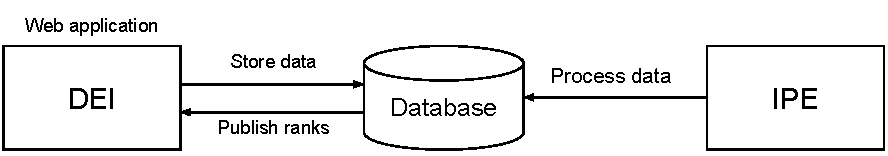
\includegraphics[width=\textwidth]{sloop/system}
  \caption{Score Distribution}
  \label{fig:sloop_overview} %chktex 24
\end{figure}

\begin{enumerate}
	\item Data Exchange and Interaction (DEI)
    DEI is a web application that provides the user interface that allows
    biologists to upload data onto sloop databases.
	\item Image Processing Engine (IPE)
    IPE processes the data stored in the databases and generate descriptors
    that represent identities of the images.
\end{enumerate}


Sloop identifies each animal on individual base. This provides the similarity
ranking of the images, within the same species, in the database relative to the
animal in a given image A. Effectiveness of such identification system heavily
depends on the choice of features on which the machine learning algorithms are
applied.

Current Sloop uses Scale Invariant Feature Transform (SIFT)~\cite{lowe04} to
perform such images ranking. Given an image and the four fiducial key points
annotated by the biologists, Sloop transforms the images into SIFT object and
compare it among the SIFTs of the existing images stored in the database, using
Euclidean distance. After the ranking is generated, the biologists then look at
the top matches and confirm whether the given pairs of images are matches or
non-matches.

While SIFT is still interesting for tasks that speed and simplicity are of
major concerns, it requires tremendous amount of manual effort and training.
Recent studies and competition results have proved that features learned via
convolutional neural networks (CNN) outperform previous descriptors, including
SIFT, on classification tasks by a wide margin~\cite{fisher14}. Therefore,
replacing SIFT with convolutional neural networks seem to be a viable
improvement to the system.

\section{Relevance Feedback}

Relevance Feedback is a technique that involves users in the retrieval process.
Specifically, given a query that returns a set of initial results, the system
takes user feedback on the initial results to improve the results returned from
the later iterations when given the same or related
query~\cite{manning2008introduction}.

\subsection{Crowdsourcing}

Crowdsourcing market is a platform takes advantage of collective intelligence
of the online community. Crowdsourcing has gained popularity as an inexpensive
and efficient method to accomplish certain tasks that are usually difficult for
machines alone to complete.

In a crowdsourcing market, there are three parties involved:
\begin{enumerate}
	\item Workers
	\item Requesters
	\item Crowdsourcing platform
\end{enumerate}

\emph{Requesters} submit tasks with the amount of \emph{reward} that they are
willing to pay \emph{workers} upon the completion of the tasks. Some workers
maybe better than others at certain tasks. In other words, some tasks maybe
more difficult than others for some workers. The platform provides the
environment for the worker and requesters to interact. All parties gain more
information about one another and the tasks, and make repeated decision
overtime.

\section{Image Recognition}

\subsection{Convolutional Neural Network}

Convolutional Neural Network is a special kind of multi-layer neural networks,
whose task is specialized to capture and encode visual patterns directly from
raw pixel images~\cite{lecun95}.

\subsection{Face Verification and Siamese Network}

The problem of finding matching image pairs from the database given an input
image, can be reduced to following \emph{decision problem}:
\begin{quote}
\centering
Given two images A and B, is the animal in image A the same individual as the
animal in image B\@?
\end{quote}

Our problem is somewhat similar to the face verification problem, which
involves accepting or rejecting an identity claim based on the image of a human
face. There are two major differences between animal identification and face
verification. First, the animal pattern has finer-grained details and some can
be very subtle that they fuse into the background. Second, the pattern of each
individual does not share same overall structure as human face does. This is
similar to identifying an identical twin by their blemishes except for, in this
case, we have very high-order of multiple births.

Most current face verification methods use hand-crafted features, which are
often combined to improve the validation performance. In~\cite{chopra05},
Chopra presented a new framework, \emph{Siamese Network}, as a solution to this
problem. He proposed a training method that is used to learn a similarity
metric from the data with the contrastive loss function, comprised of the sum
of the \emph{magnitude of the difference between the features vectors} of the
incorrect guesses. This loss function encourages matching pairs to be close
together in feature space while pushing non-matching pairs apart. However, it
may not be the best option in our case because the difference in each feature
contributes equal weight to the loss, whereas in our model, each feature may
require different weights in the loss function that is not proportional to the
weight learned in the convolutional network.

% chapter related_work (end)

% Related Liturature and Studies
% * Organzied to cover specific problem
% * how it helps the current study/how it relates
%!TEX root = main.tex
\graphicspath{{images/chap3/}}
% Relevance Feedback
% Methodology
% * Design and Architecture
% * Population of interest and sampling subject used in the study
% * Instrument and what it measures (matrices)
% * qualifications of informants if used in the study
% * Validation
% * Data gathering procedure (experiments)
\chapter{Datasets} % (fold)
\label{cha:datasets}

All the experiments in this study are conducted on a database which comprises two
species of skinks: \emph{Grand} and \emph{Otago} of 3687 images in total
created by biologists at New Zealand's Department of Conservation.

\begin{figure}[htb]
  \centering
  \begin{subfigure}[t]{0.31\textwidth}
      \centering
      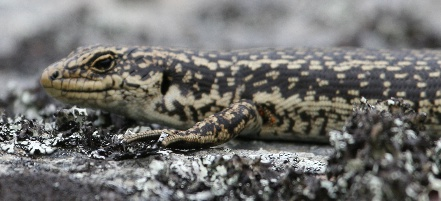
\includegraphics[width=4.5cm]{dataset/general/grand_L3}
  \end{subfigure}
  \begin{subfigure}[t]{0.31\textwidth}
      \centering
      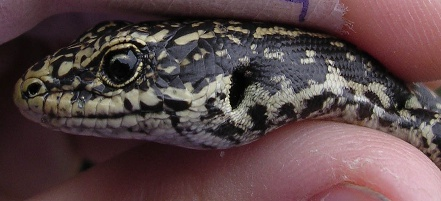
\includegraphics[width=4.5cm]{dataset/general/grand_L1}
  \end{subfigure}
  \begin{subfigure}[t]{0.31\textwidth}
      \centering
      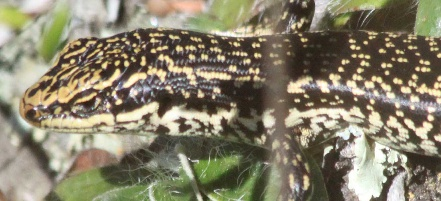
\includegraphics[width=4.5cm]{dataset/general/grand_L2}
  \end{subfigure}
  \captionsetup{justification=centering}
  \caption{Left view images from Grand dataset}
  \label{fig:grand_left} %chktex 24
\end{figure}

\begin{figure}[htb]
  \centering
  \begin{subfigure}[t]{0.31\textwidth}
      \centering
      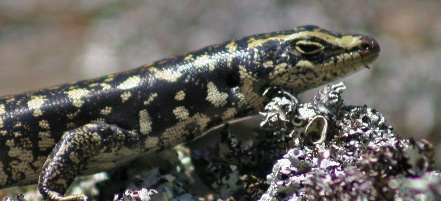
\includegraphics[width=4.5cm]{dataset/general/otago_R2}
  \end{subfigure}%
  \begin{subfigure}[t]{0.31\textwidth}
      \centering
      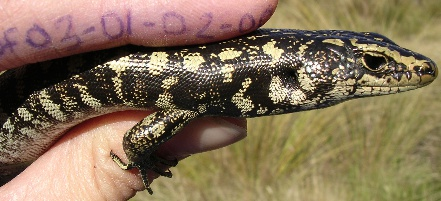
\includegraphics[width=4.5cm]{dataset/general/otago_R1}
  \end{subfigure}
  \begin{subfigure}[t]{0.31\textwidth}
      \centering
      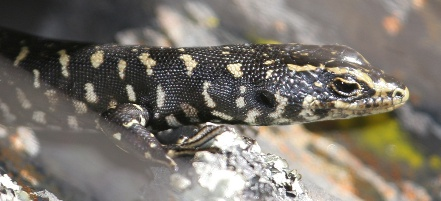
\includegraphics[width=4.5cm]{dataset/general/otago_R3}
  \end{subfigure}
  \captionsetup{justification=centering}
  \caption{Right view images from the Otago dataset}
  \label{fig:otago_right} %chktex 24
\end{figure}

The Grand database contains 1871 \texttt{RGB} images of 206 individuals, while
the Otago database contains 1816. These images vary in size, lighting, and
background. The images are closely cropped to include only the anterior end of
their subjects. The size varies from 1056 $\times$ 564 to 2437 $\times$ 1215
pixels.

\begin{table}[htb]
\captionsetup{justification=centering}
  \caption{Summary of each database}
  \label{tab:database_summary} %chktex 24
  \centering
  \begin{tabular}{lccccccc}
    \toprule
    & \multicolumn{3}{c}{Number of Images} & & &
        \multicolumn{2}{c}{Images per Individual} \\
    \cmidrule{2-4}
    \cmidrule{7-8}
    Name & Left View & Right View & Total & Individuals & Singletons & Avg.
        & Max. \\
    \midrule
    Grand & 929 & 942 & 1871 & 206  & 69 & 9 & 31 \\
    Otago & 903 & 913 & 1816 & 221  & 58 & 8 & 24 \\
    \bottomrule
  \end{tabular}
\end{table}


\section{General}

\subsection{Selfscore and Score Distributions}

Sloop ranks the likelihood that two capture events contain the same individuals
quantitatively by \emph{similarity score}. The similarity score between two
individuals is obtained from comparing the SIFT features of all the images
within a capture to the SIFT features of the images within the other
individual's cohort.  These scores are normalized by the \emph{minimum
selfscore} among all the images involved in the
comparison. A \emph{capture} is a group of images containing the same
individual from different views, captured at the same time.  A \emph{cohort} is
a set of all images from all captures of the same individual.

\subsubsection{Selfscores}

The selfscore for a capture is the \emph{maximum} selfscore of all the images within
the capture, where a selfscore of an image is calculated from comparing the
sift features of each image with itself.
$$\texttt{selfscore}(C) = \max_{\forall I_i \in C} \texttt{sift\_match}(I_i, I_i)$$

\begin{figure}[htb]
   \centering
    \begin{subfigure}[t]{0.6\textwidth}
        \centering
        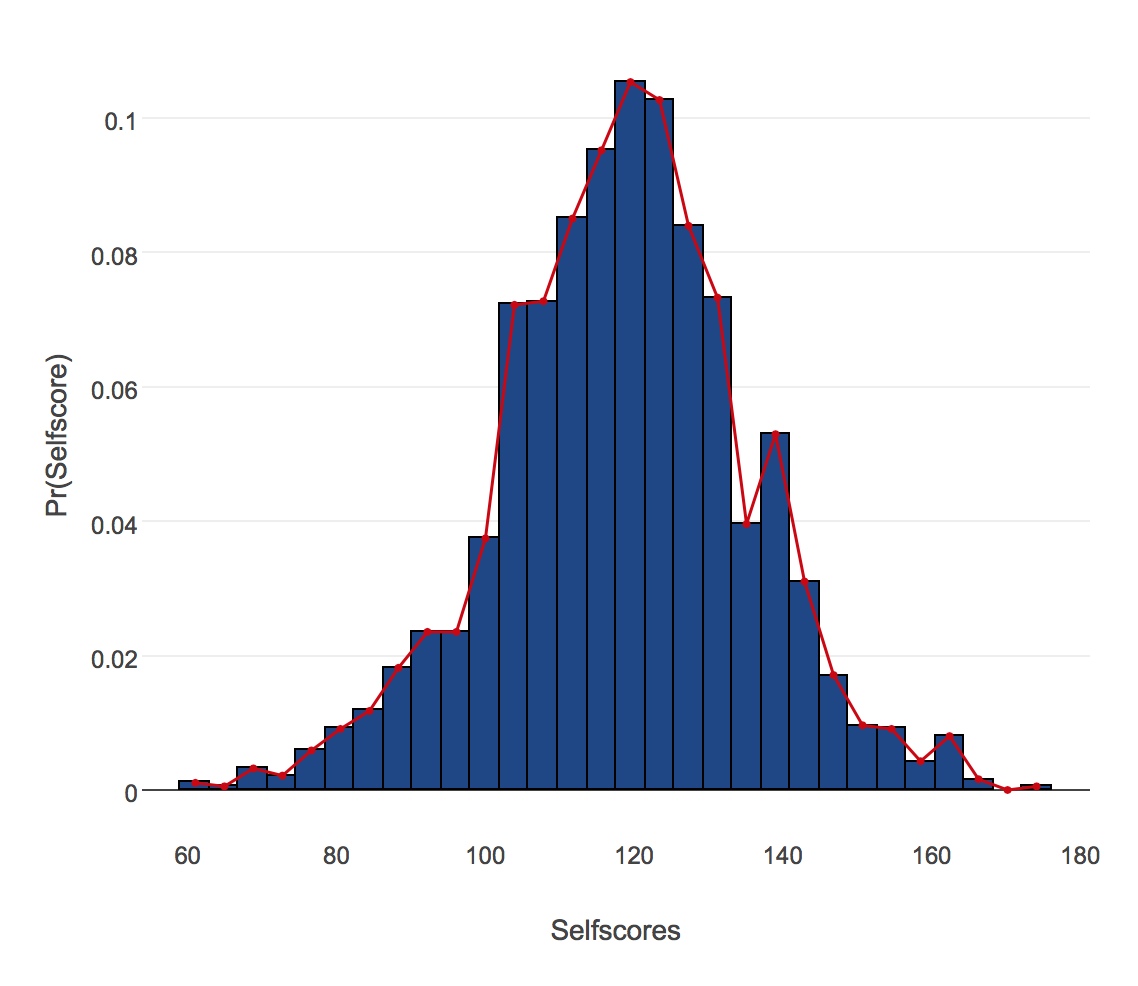
\includegraphics[height=2.5in]{dataset/grand/selfscores}
        \caption{Probability distribution}
    \end{subfigure}%
    \begin{subfigure}[t]{0.35\textwidth}
        \centering
        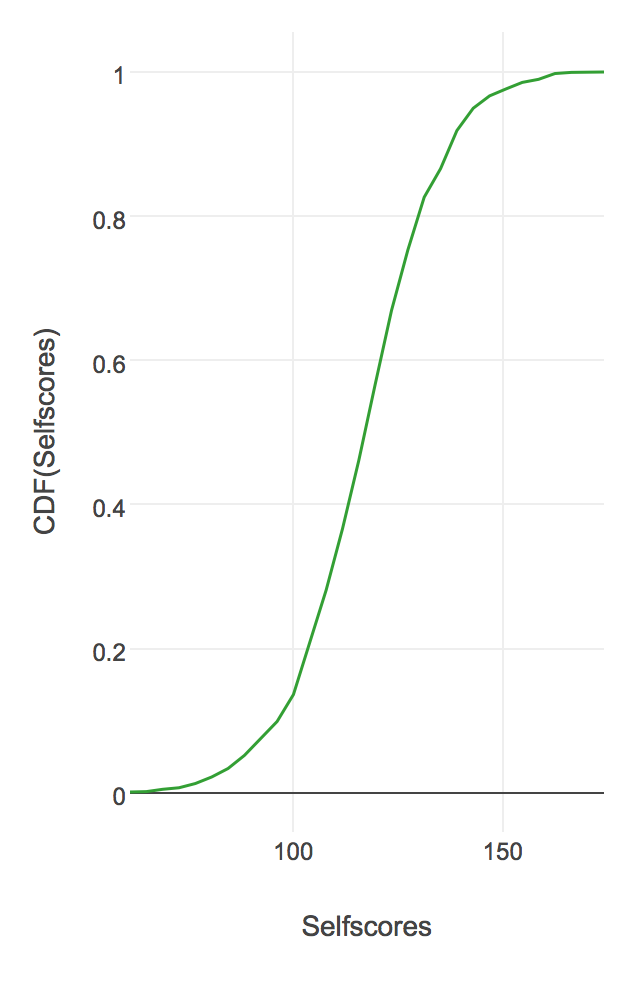
\includegraphics[height=2.5in]{dataset/grand/cdf_selfscores}
        \caption{Cumulative probability distribution}
    \end{subfigure}
    \caption{Grand selfscores}

    \begin{subfigure}[t]{0.6\textwidth}
        \centering
        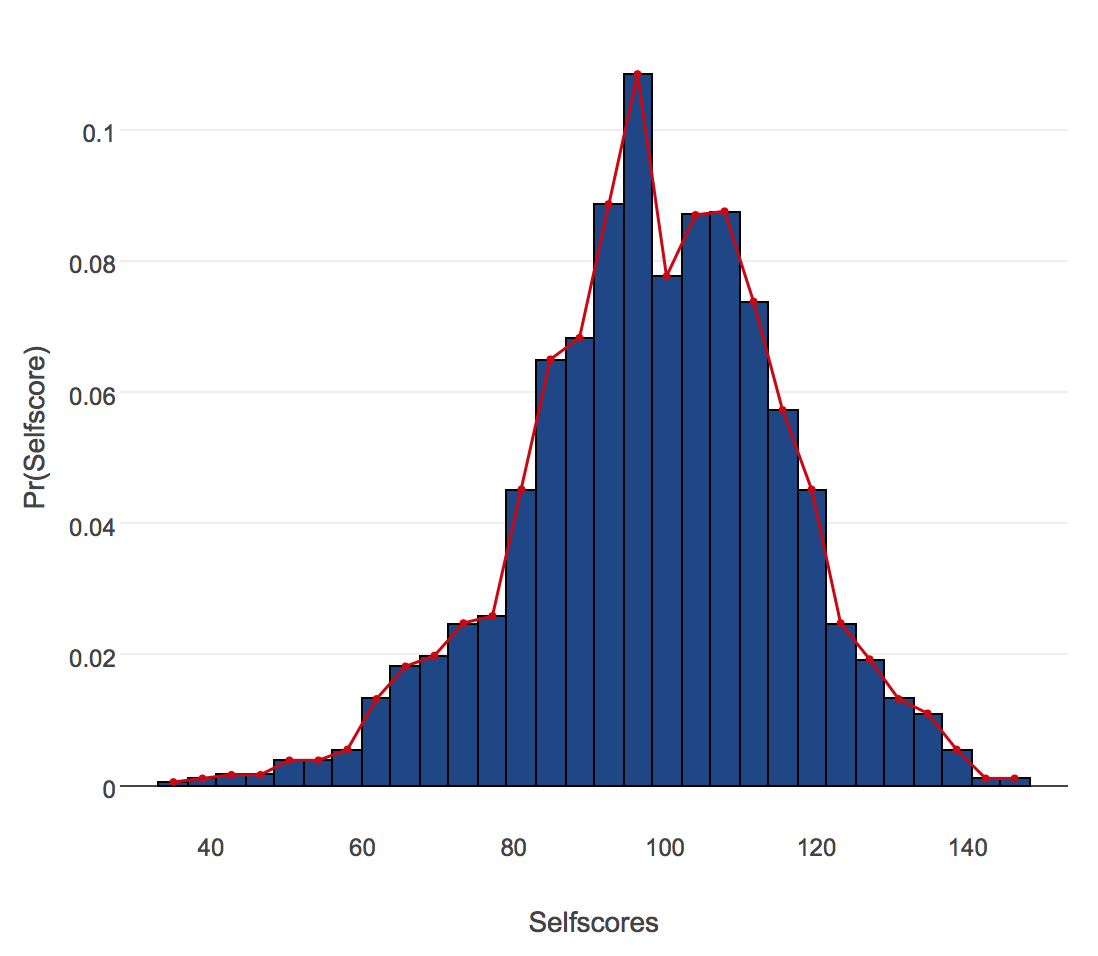
\includegraphics[height=2.5in]{dataset/otago/selfscores}
        \caption{Probability distribution}
    \end{subfigure}%
    \begin{subfigure}[t]{0.35\textwidth}
        \centering
        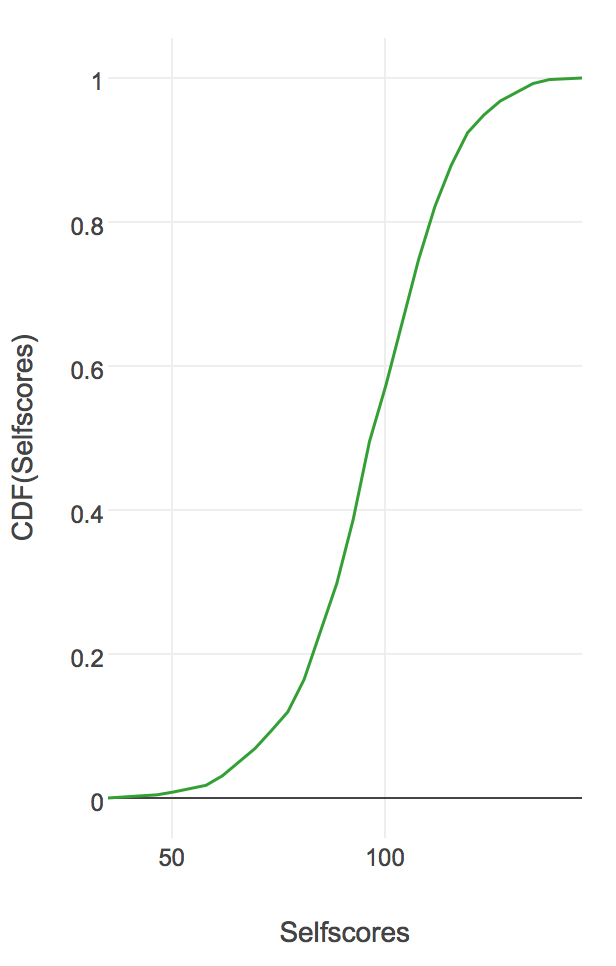
\includegraphics[height=2.5in]{dataset/otago/cdf_selfscores}
        \caption{Cumulative probability distribution}
    \end{subfigure}
    \caption{Otago selfscores}
\end{figure}

\subsubsection{Scores}

The score between the two individuals is the maximum score among all the
comparisons among the images within the two cohorts.
$$\texttt{score}(C_1, C_2) = \max_{\forall I_i \in C_1 \forall I_j \in C_2}
    \frac{\texttt{sift\_match}(I_i, I_j)}{\min(\texttt{selfscore}(C_1),
        \texttt{selfscore}(C_2))}$$
where $C$ is a capture and $I$ is an image in a capture.

\begin{figure}[htb]
 \begin{subfigure}[t]{\textwidth}
  \centering
  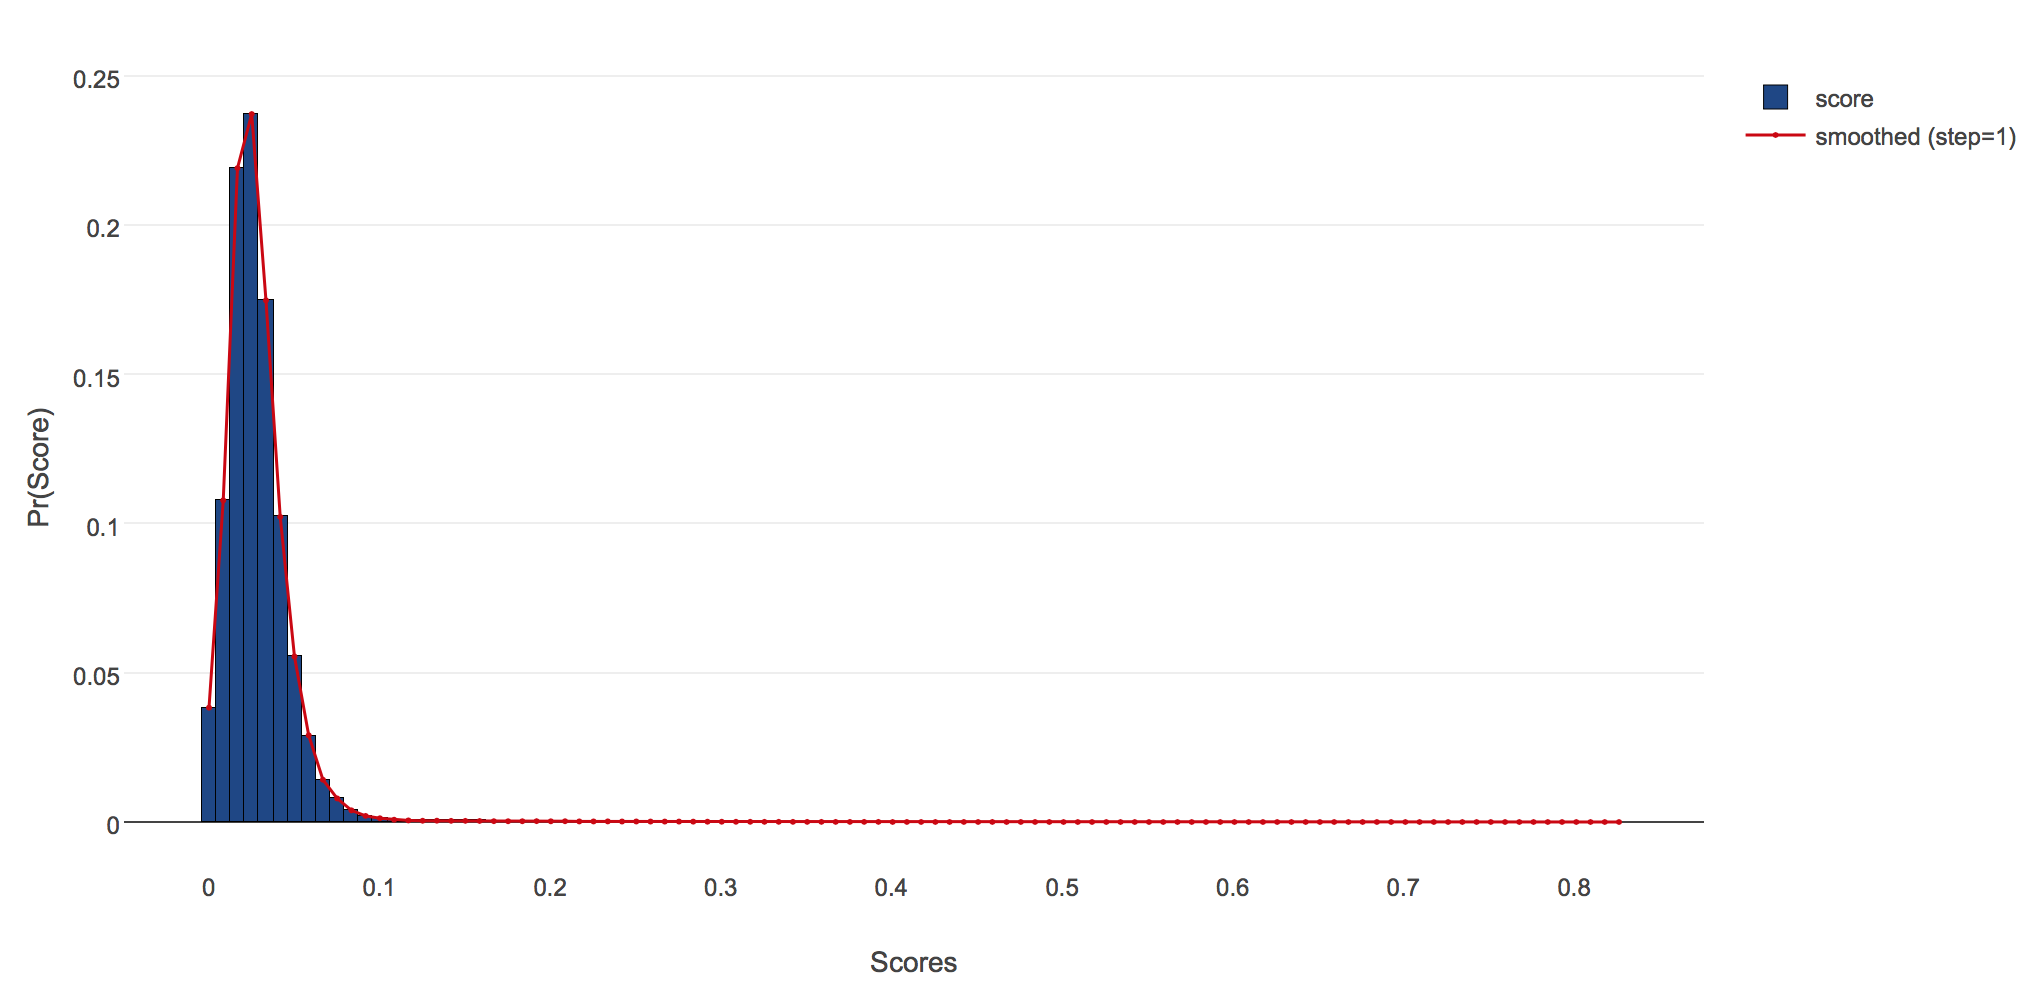
\includegraphics[height=2.7in]{dataset/grand/scores}
  \caption{Grand Score Distribution}
  \label{fig:grand_scores} %chktex 24
\end{subfigure}

 \begin{subfigure}[t]{\textwidth}
  \centering
  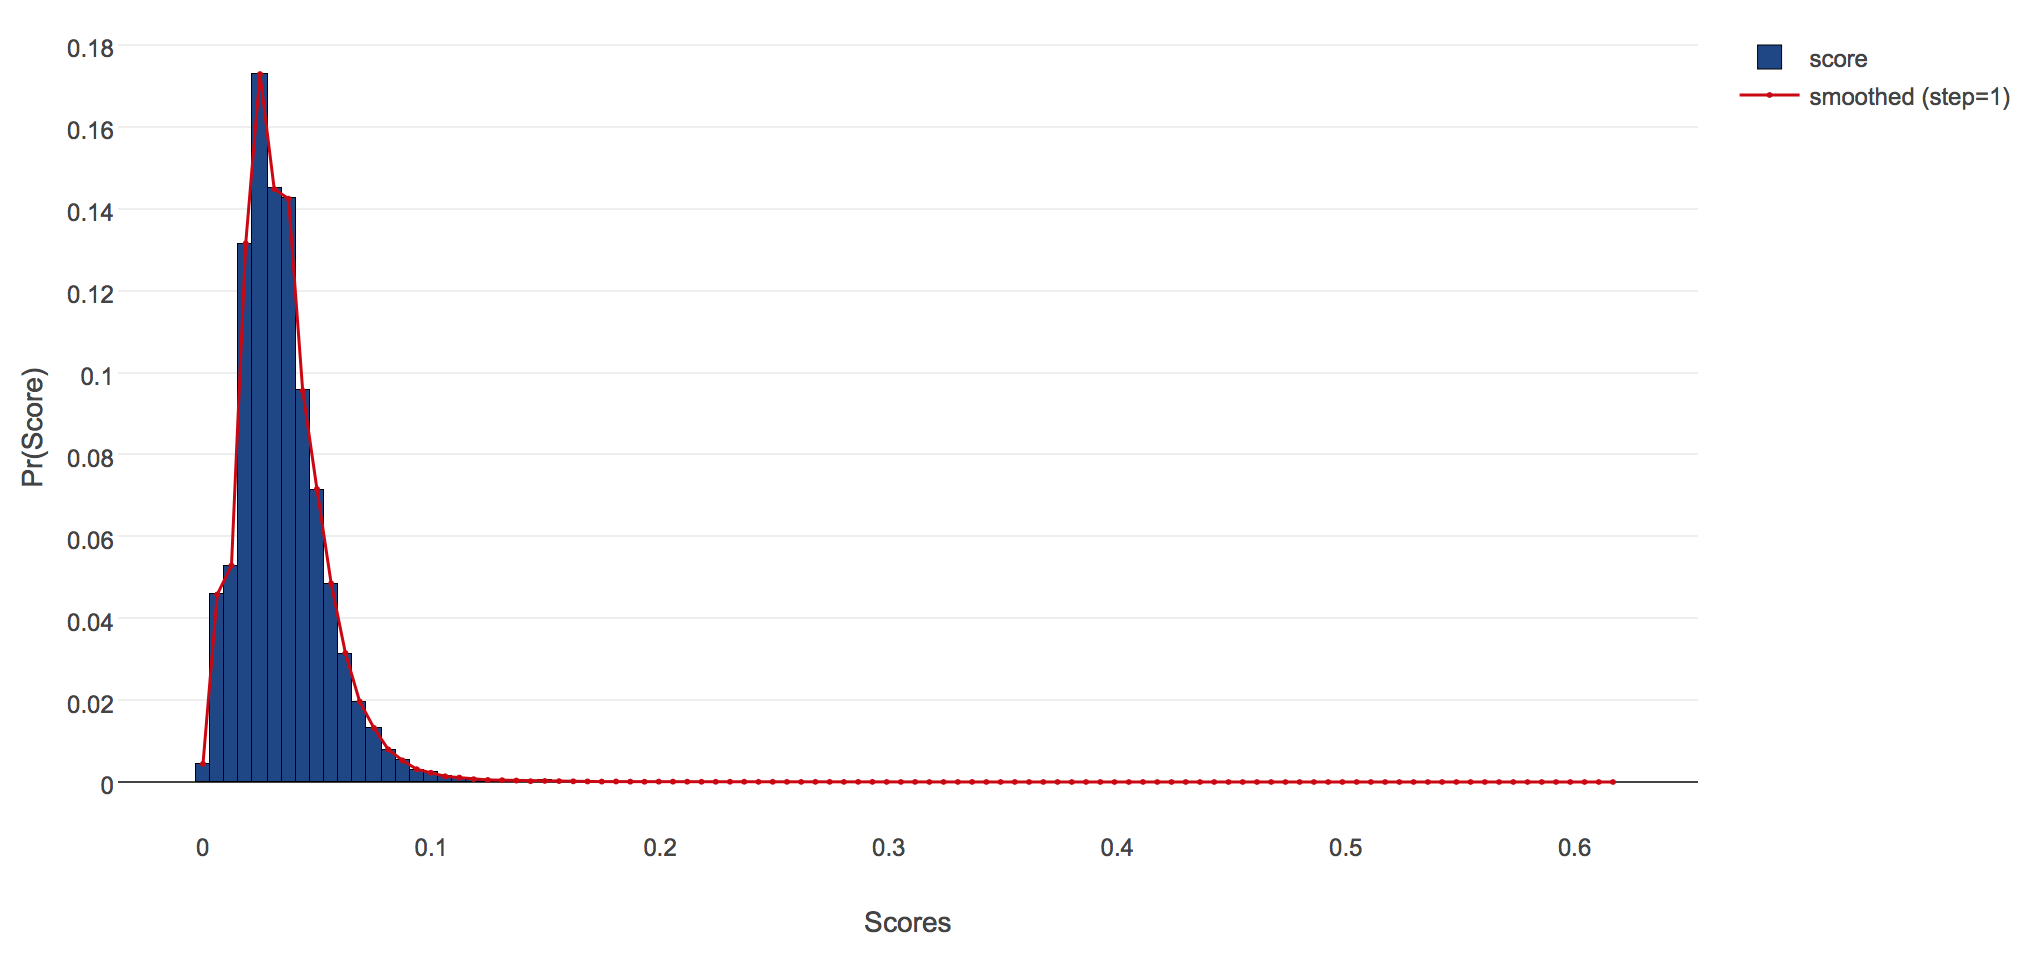
\includegraphics[height=2.5in]{dataset/otago/scores}
  \caption{Otago Score Distribution}
  \label{fig:otago_scores} %chktex 24
  \end{subfigure}
\end{figure}

% Relevance Feedback: Relevance feedback accelerates recall
% Methodology
% * Design and Architecture
% * Population of interest and sampling subject used in the study
% * Instrument and what it measures (metrices)
% * qualifications of informants if used in the study
% * Validation
% * Data gathering procedure (experiments)
\graphicspath{{./images/chap4/}}
% Relevance Feedback
% Methodology
% * Design and Architecture
% * Population of interest and sampling subject used in the study
% * Instrument and what it measures (metrices)
% * qualifications of informants if used in the study
% * Validation
% * Data gathering procedure (experiments)
\chapter{Relvance Feedback}
\label{chap:relevance_feedback}

To study and understand the effect of relevance feedback to the retrival
results, we implement a simulator that reproduces the relevance feedback
processes of sloop. The implementation of the simulator is described in
\ref{sec:method} section. We then compare the initial ranked result set
outputted from SIFT computation with the results that undergo different rounds
of relevance feedback with various configurations in the \ref{sec:experiments}
section.

\section{Methodology}
\label{sec:method}

The relevance feedback simulator mimics the behavior of the task submission
process by the repeatedly sampling a batch of capture pairs from the pool of
all unknown capture pairs. For all the sampled pairs within a batch, the
simulator marks them as matching pairs or non-matching pairs with the
\emph{correct} answers.

When all the pairs in a specific batch are marked, it constructs an
\emph{identity graph} that represents the connections between all the known
pairs using the marked answers. The identity graph is undirected. The nodes in
the graph represent captures. If there is an edge connecting between node $A$
and $B$, capture $A$ and $B$ contain the same individual. Graphically mapping
the relationship of individuals results in fully-connected subgraphs formed by
all the captures containing the same animals.

Upon the retreival of the new information from each batch, the simulator uses
the identity graph to infer the answers of the unknown pairs. This imitates the
in-database merging logic of the current version of Sloop\cite{sloopdocs}. The
transitive relations are drawn from both matching pairs and non-matching pairs.
For example, given capture $A$ is known to contain the same individual as that
in capture $B$, and capture $B$ is known to contain the same individual as that
in capture $C$, the simulator can infer that capture $A$ contains the same
individual as that in capture $C$, without having known the actual answer of
$A$ and $C$. Once such transitive interence is made, it adds $C$ to the
identity graph. Then, it continues to sample a new batch iteratively until the
distribution satisfies the convergence condition specified by the user.

The inferred decision plays a very crucial role in relevance feedback. The
validity of such inference relies on the validity of the premises. If the
answers to the matches are correct then the conclusion must be true. Problems
arise when our seemingly \emph{correct} answers are in fact incorrect. In the
actual production of Sloop, the inconsistence results from such error is
detectable and will be submitted for manual review. However, in the simulation,
we would like to also examine the consequences of the incorrect answers. With
the auto merging, the error propagates rapidly. Therefore, the simulation
allows users to specify the error probability at the initialization.

\section{Metrices} % (fold)
\label{sec:metrices}

This section describes the metrices used to evaluate the performance our
models. Along with our goal to maximize the precision and recall, we would like
to minimize the cost of the crowdsed feedback or to operate optimally within a
budget constraint. The simulator also provides a counter that counts the number
of iterations a distribution takes to converge. However, this is out of our
interest because the time a model takes to converge can also be inferred from
the number of task submitted. Given a model, the fewer assignments posted, the
faster the model converges. 

\subsection{Precision and Recall} % (fold)
\label{sub:precision_and_recall}

As you can see, in the system where true negatives (true non-matching pairs)
largely outnumbers the true positives (true matching-pairs), comparing the
\emph{true positive rate (TPR)} or recall to the \emph{false positive rate
(FPR)} is not very meaningful. This is because false positive rate, which is
$\Pr{(\hat{y}=1|y=0)} = \frac{FP}{FP+TN}$, is going to be approximately 0 as
$TN$ is very large. Thus, instead of using ROC (receiver operating
characteristic) curve, which is a plot of TPR and FPR, we use
\emph{precision-recall curves (PR)} to analyze the performance of our models.

A precision recall curve is a plot of precision and recall as we  vary the
threshold $\theta$. Precision or positive predictive value (PPV) is defined as
following \cite{manning2008introduction}: $$PPV = \Pr{(y=1|\hat{y}=1)} =
\frac{TP}{\hat{P}} = \frac{TP}{TP+FP}$$

We evaluate the ranked retrieval performance of diffrent relevance feedback
sampling policies using the \emph{Mean Average Precision (MAP)}, which is
roughly the area under the \emph{precision-recall curves}.
% subsection precision_and_recall (end)

\subsection{Cost} % (fold)
\label{sub:cost}

The total amount of money we have to spend to reward the workers is
proportional to the \emph{number of tasks we published}. If, at the moment we
have just finished marking all the unknown pairs, there are still some leftover
tasks on the crowdsourcing, those tasks are not going to be cancelled (unless
the user forcefully cancels the tasks himself.) Hence, we can use the number of
tasks we published as our cost metric.
% subsection cost (end)

% section metrices (end)

\section{Experiments} % (fold)
\label{sec:experiments}

In this section, we consider a setting in which time evolves in rounds. In each
round, the we, the requester, simulates the task submission process in a
crowdsourcing platform assuming that all the workers completes all the task.
Our goal as the requester is to maximize the Mean Average Precision value of a
preliminary score distribution outputted from Sloop with the amount payments we
have to make in mind.

We report three experiments corroborating the improvement of the retreival
results after various rounds of relevance feedback and different sampling
strategies.  Experiment \ref{sub:batch_sizes} establishes that relevance
feedback improves the acceration of precision and recall of the preliminary
results at various batch sizes.  Experiment \ref{sub:errors} shows the
consequence of the errorneous answers at diffferent error probabilities.
Experiment \ref{sub:sampling_policies} compare the performance of various
sampling policies.

All experiments are performed on the Grand and Otago dataset described in
Chapter \ref{cha:datasets}. Both datasets are annotated by the biologist, which
we take as our true labels. Table 

\begin{table}[t]
\captionsetup{justification=centering}
  \caption{Number of capture pairs for each species}
  \label{species-num-pairs}
  \centering
  \begin{tabular}{lc}
    \toprule
    Species & Number of pairs \\
    \midrule
    Grand & 507528 \\
    Otago & 492690 \\
    \bottomrule
  \end{tabular}
\end{table}

\subsection{Batch Sizes} % (fold)
\label{sub:batch_sizes}

This experiment first shows that relevance feedback improves the acceration of
precision and recall of the preliminary results at different iterations and
batch sizes. To establish these relations, we randomly sample some unknown
pairs from our unknown pair pool using \emph{uniform} sampling policy, in which
drawing each unknown pair is equally probable. The reason we use uniform random
sampling policy is because it is simple and unbiased, which is useful to get a
general baseline value.

During the sampling process, we observe the Mean Average Precision (MAP) at
each iteraion. A batch of samples is iteratively drawn until we know the
answers to \emph{all} the unknown pairs or MAP is equal to 1, whichever happens
first.

We then repeat the process for various batch sizes, which is defined to be the
total number of unknown pairs marked in between a pair of the following events:
initialization, identity inference, and termination. Finally, we compare the
number of pairs sampled to reach convergence for each batch size.
% subsection batch_sizes (end)

\subsection{Errors} % (fold)
\label{sub:errors}

Despite the tasks distribution and the gold standard questions, there is
probability of 0.078 of obtaining an incorrect answer, assuming that all the
preventive events are independent. However, in practice, errors occur
haphazardly rather than systematically. Thus, 0.078 is the worst case, where we
assumed the worker always make a guess with equal probability.

This experiment models such error. Given an error probability of $\epsilon$, if
a pair of captures is sampled, the simulator marks it with the annotated answer
(correct answer) with the probability of $1-\epsilon$; otherwise, the pair is
marked with the opposite label (incorrect answer). Again, we compare the values
of MAP at each iteration and the total number of pairs sampled for each error
probability.
% subsection errors (end)

\subsection{Sampling Policies} % (fold)
\label{sub:sampling_policies}

Sampling policy plays a significant role in the retrieval. Given an initial
ranking, a pair of captures whose score is within a certain range or higher
than certain threshold is more likely to be a match. Such range and threshold
is species-specific and relies on Sloop's classification performance.

We experiment with following policies:
\begin{description}
  \item [Uniform]
  Sample an unknown pair from a uniform distribution where drawing each
    \emph{pair} is equally probable.
  \item [UniformScore]
  Sample an unknown pair from a uniform score distribution where drawing a pair
    with each \emph{score} is equally probable.
  \item [TopMatches]
  Always select an unknown pair with the highest score.
  \item [Nonmatches]
  Always select an unknown pair with the lowest score.
  \item [Normal]
  Sample an unknown pair from a normal distribution with $\mu=$median and
    $\sigma=0.3$.
  \item [Percentile]
  Always select an unknown pair at the median.
  \item [AllScores]
  Divide the scores into $n$ bins, where $n=$\texttt{batch\_size} and then
  select some unknown pairs from all the bins so that the total number of
  unknown pairs sums to \texttt{batch\_size}.
\end{description}

% subsection sampling_policies (end)

% section experiments (end)

\section{Results and Discussion} % (fold)
\label{sec:results}

Figure \ref{pr-curves} displays the Precision-Recall graph at a given number of
sampled unknown pairs. With zero error probability, relevance feedback reduces
the number of comparisons required for each specifies by a factor of 317 and
307 for grand and otago respectively. Within four iterations of feedback loop,
Mean Average Precision (MAP) reaches 1.0.

The results corroborates the fact that the relevance feedback dramatically
accerates precision and recall given the correct feedback information. Such
inclination of precision and recall is expected largely due to the
interpolation of the new information.

\begin{figure}[h!]
  \label{pr-curves}
  \centering
  \subfloat[Grand]{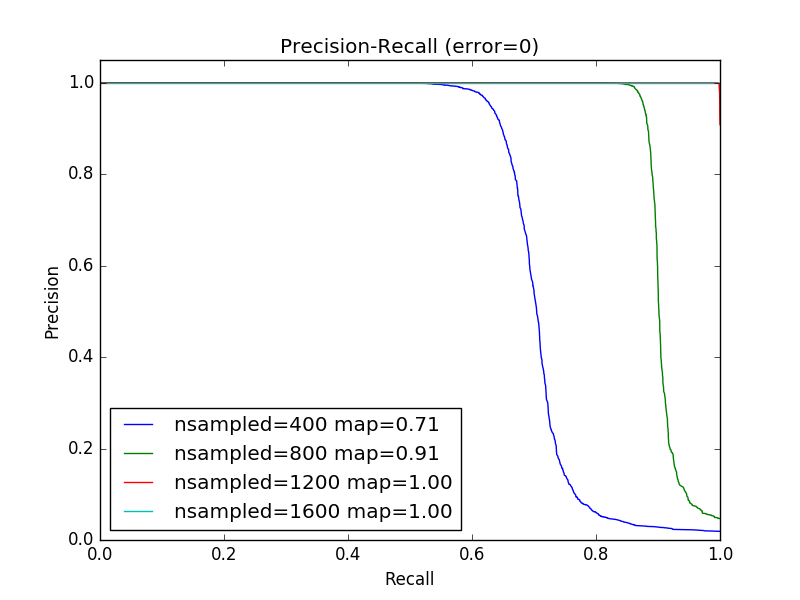
\includegraphics[width=0.8\textwidth]{pr/grand}}\\
  \subfloat[Otago]{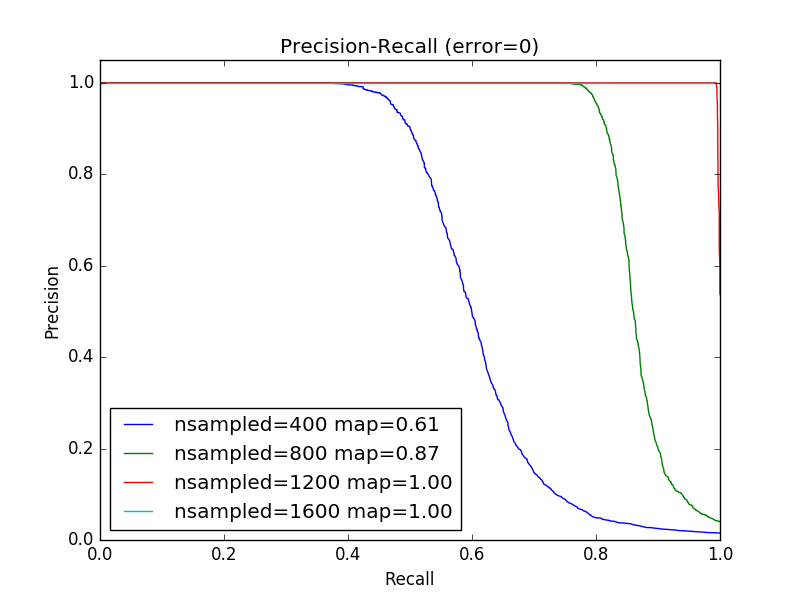
\includegraphics[width=0.8\textwidth]{pr/otago}}
  \captionsetup{justification=centering}
  \caption{Precision-Recall graph ($Error=0$, \texttt{batch\_size}$=400$)}
\end{figure}

\subsection{Batch Sizes} % (fold)
\label{sub:batch_sizes_res}

Overall, from the graphs, MAP increases as we feed more data into the system.
Figure \ref{fig:batchsizegraph} indicates that we publish more uneccessary
tasks as we increase the batch size. The fewer captures there are in a batch,
the lower the overall cost. Taking this idea one step further, we would like to
infer the matches and merge the individuals as frequently as possible. However,
empirically, smaller batch size may upset some workers who would like to
continuously work on the tasks. Therefore, we need to find the smallest batch
size that is still large enough to engage the workers.

\begin{figure}[h!]
  \centering
  \subfloat[Grand]{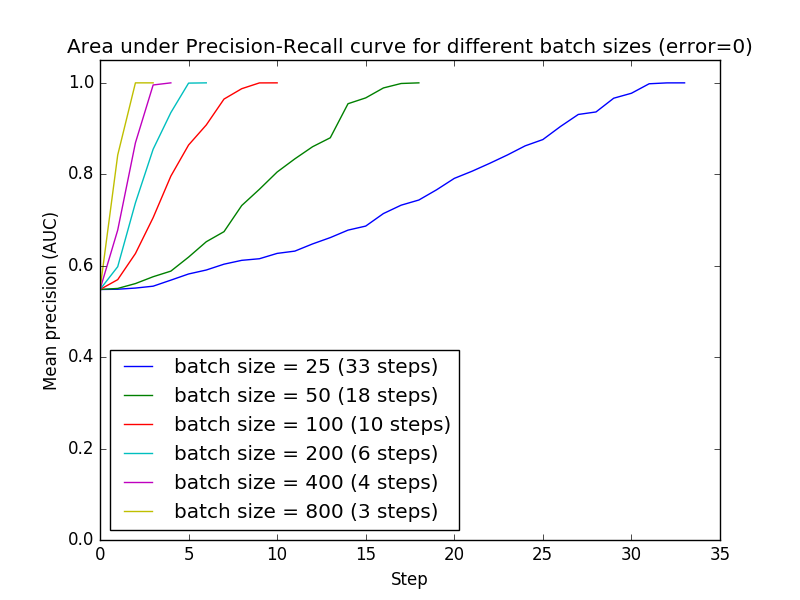
\includegraphics[width=0.8\textwidth]{sizes/graoc}}\\
  \subfloat[Otago]{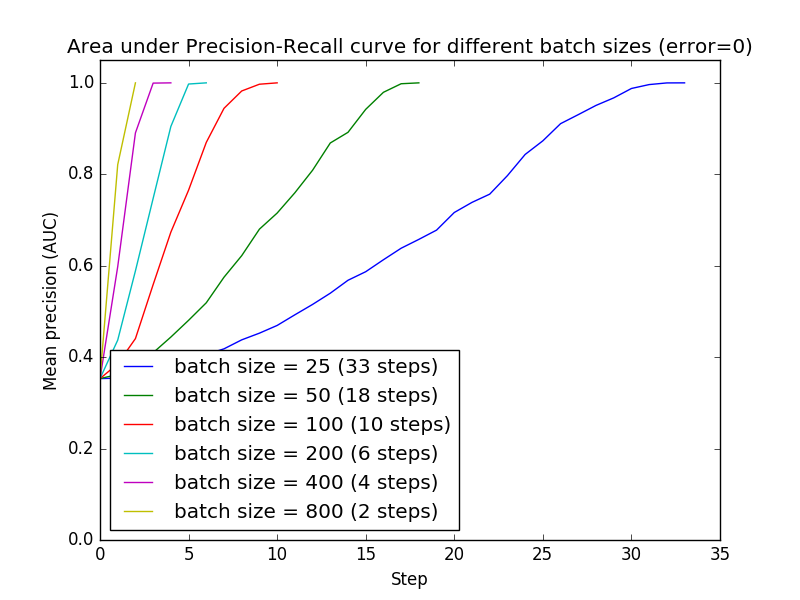
\includegraphics[width=0.8\textwidth]{sizes/otaoc}}
  \captionsetup{justification=centering}
  \caption{Mean Average Precision (MAP) for different batch sizes ($Error=0$)}
\end{figure}

\begin{figure}[h!]
  \label{fig:batchsizegraph}
  \centering
  \subfloat[Grand]{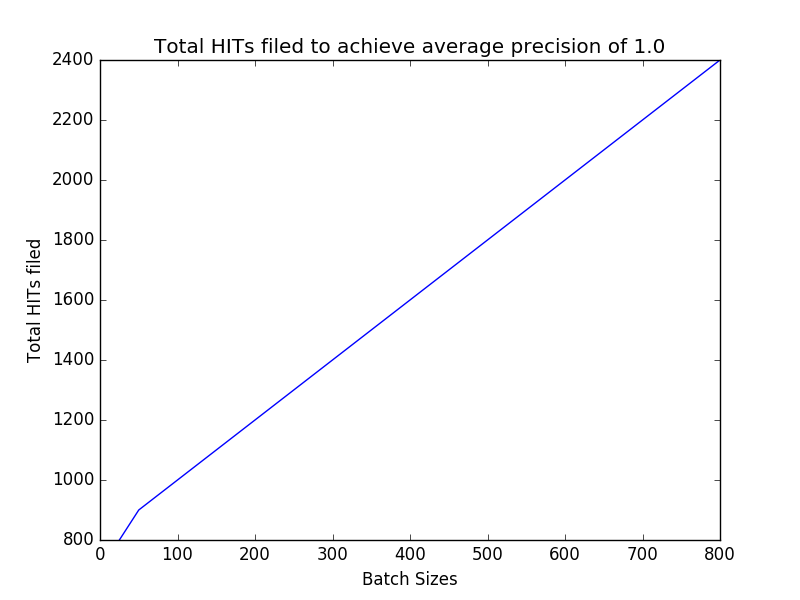
\includegraphics[width=0.8\textwidth]{sizes/grtotal}}\\
  \subfloat[Otago]{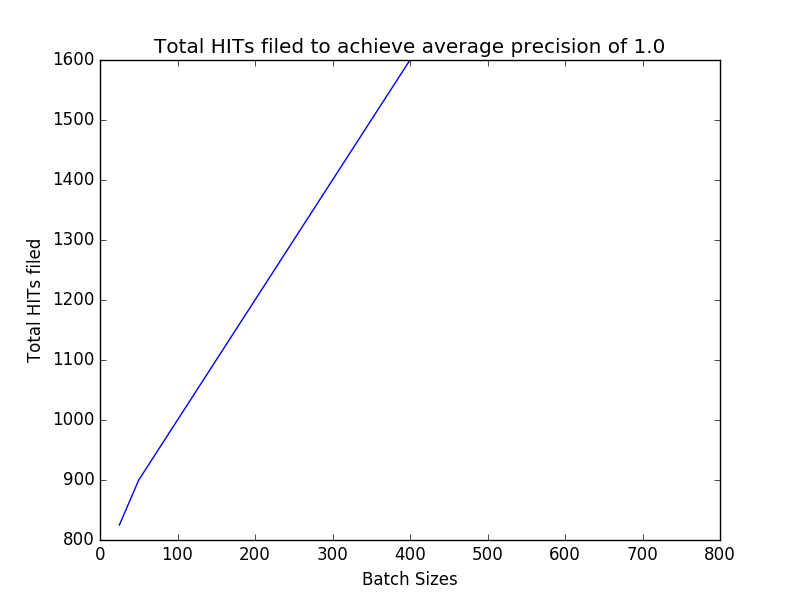
\includegraphics[width=0.8\textwidth]{sizes/ottotal}}
  \captionsetup{justification=centering}
  \caption{The total number of unknown pairs marked to achieve $MAP=1$
  ($Error=0$, \texttt{batch\_size}$=100$). Notice that this equals the total 
  number of tasks published to achieve $MAP=1$. }
\end{figure}

% subsection batch_size (end)

\subsection{Errors} % (fold)
\label{sub:errors_res}

Despite the present of errors, relevence feedback still yields higher MAP
overall with an error threshold of 0.05. With a nonzero error probability, MAP
curves downward before it curves up and reach a saturation point. This is
because initially when it does not have much data, the system is very sensitive
to errors, especially the false negatives, which trigger the irreversible merge
operation. Thus, the precision decline rapidly.  As it gains more correct data,
it is able to recover from the downward phase. However, the historical merges
resulted from the past faulty data are irrevocable, so the precision saturates
eventually.

\begin{figure}[h]
  \centering
  \subfloat[Grand]{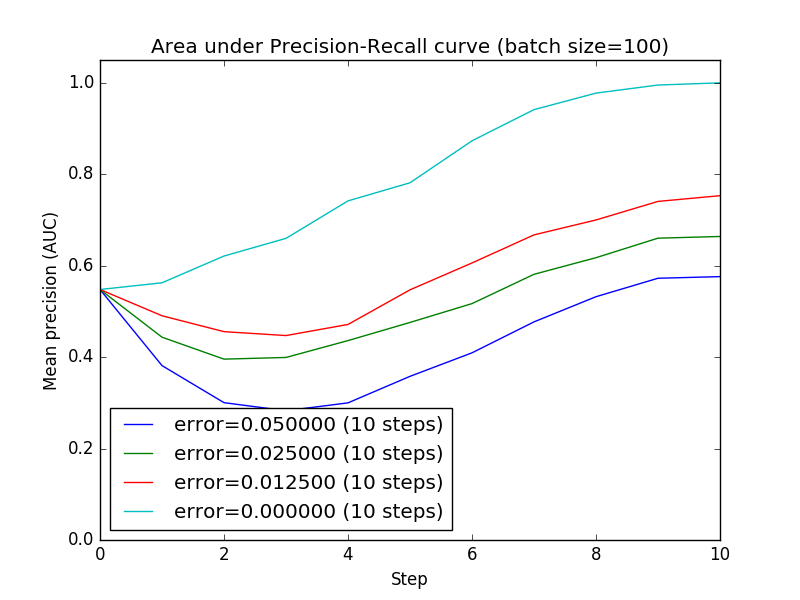
\includegraphics[width=\textwidth]{errors/graoc}}
  \caption{Mean Average Precision for different probabilities of error}
  \label{fig:overview}
\end{figure}

% subsection errors (end)

\subsection{Sampling Policies} % (fold)
\label{sub:sampling_policies_res}

Uniform sampling (Uniform), normal sampling (Normal), and sampling from all the
scorces (AllScores) seem to outperform other sampling policies in term of the
total cost. The samplers that sample single score values at a time, such as
sampling from median (Percentile), performs poorly compare to others. However,
this depends largely on the species of the animal that we are interested in. As
you can see the performance of the each sampling policy differs slightly
between grand and otago.

\begin{figure}[h!]
  \centering
  \subfloat[Grand]{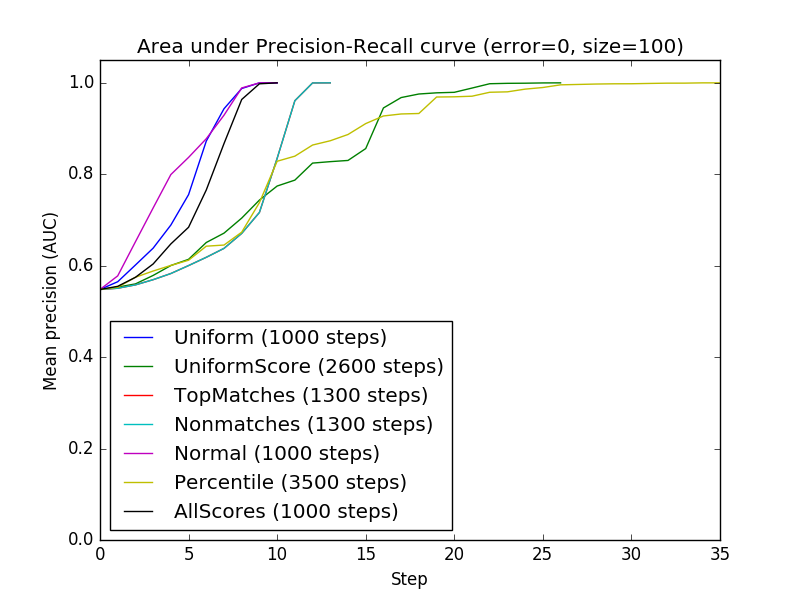
\includegraphics[width=0.8\textwidth]{policies/grand}}\\
  \subfloat[Otago]{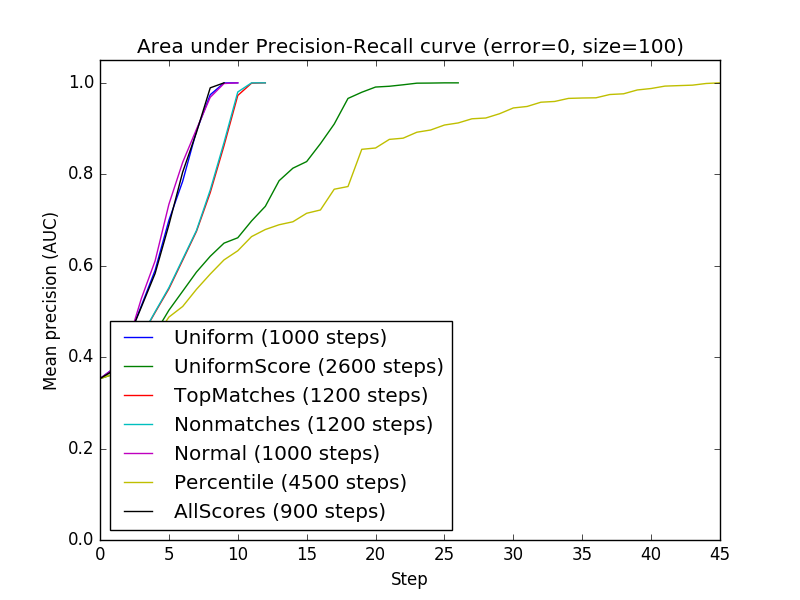
\includegraphics[width=0.8\textwidth]{policies/otago}}
  \captionsetup{justification=centering}
  \caption{Mean Average Precision (MAP) for various sampling policies ($Error=0$, \texttt{batch\_size}$=100$)}
\end{figure}

% subsection sampling_policies (end)

% section results (end)

% Sloop-mturk: Crowdsourced relevance feedback on mturk
% Methodology
% * Design and Architecture
% * Population of interest and sampling subject used in the study
% * Instrument and what it measures (metrices)
% * qualifications of informants if used in the study
% * Validation
% * Data gathering procedure (experiments)
%!TEX root = main.tex
\graphicspath{{images/chap5/}}
% Sloop-mturk: Crowdsourced relevance feedback on mturk
% Methodology
% * Design and Architecture
% * Population of interest and sampling subject used in the study
% * Instrument and what it measures (metrics)
% * qualifications of informants if used in the study
% * Validation
% * Data gathering procedure (experiments)
\chapter{Crowdsourced Relevance Feedback}
\label{chap:sloop_mturk}
% Sloop-mturk: Crowdsourced relevance feedback on mturk

As described in Chapter~\ref{chap:relevance_feedback}, multiple rounds of
relevance feedback accelerates precision and recall. Such feedback can be 
obtained through various approaches at different costs. We could send all
the system's peliminary results to the biologists to verify the matches.
However, this option is impossible to implement on a large scale and costly
because clearly their time would have been better spent elsewhere.

Instead, we utilize \emph{crowdsourcing} markets to efficiently gather
feedback. The markets provide repeated interaction between requesters and
workers, enabling us to obtain solutions to simple human-friendly tasks that
are difficult for computers to solve. However, taking an account of the cost
requires the acceptance of any necessary trade-offs between quality and
quantity. To alleviate this problem, we need an
effective quality control policy so that workers, requesters, and the platform
itself can all adjust their behavior over time. 

This chapter explains crowdsourcing within Sloop and later presents the
architecture of \emph{Sloop MTurk}, the crowdsourced relevance feedback engine
for Sloop.

\section{Crowdsourcing} % (fold)
\label{sec:crowdsourcing}

  \subsection{Platform Selection}

  Workers and requesters interact via a crowdsourcing platform. There are several 
  platforms available, each with a diffferent focus. Examples of such
  platforms are 
  Amazon Mechanical Turk, which focuses on a series of small repetitive
  tasks~\cite{sliv14}; Microsoft's Universal Human Relevance System (UHRS),
  whose tasks mainly involve organizing online contents;
  and Upwork, which focuses on larger projects that requires programming skill.
  % TODO explain why we choose MTurk
  All our tasks are published on Amazon Mechanical Turk (MTurk), which is one of the most
  popular crowdsourcing platforms.

  \subsection{Human Intelligence Tasks (HITs)}

  Tasks published on MTurk are called Human Intelligence Tasks (HITs). The terms
  `HIT' and `task' will be used interchangeably throughout this report.

  Requesters publish the tasks that they need completed to Amazon Mechanical
  Turk's marketplace with a set payment to reward workers who finish the tasks.

  \subsubsection{Task Design}

  A wide variety of tasks can be crowdsourced. There are two possible designs we
  have considered:
  \begin{enumerate}
	\item Rankings and weights \\
    Each worker may be asked to provide a full ranking or relative weights
    for a given pool of candidates. Although knowing the correct rankings is
    valuable to ranked retrieval results,
    ultimately, we would like to determine a sharp cutoff between matching
    images and non-matching images so that each individual can be exclusively
    identified. Ranks alone do not provide such a cutoff. Even if we knew all the
    correct rankings, we would not be able to decide whether two animals are
    the same individual. Thus, rankings and weights is not a viable
    solution.
	\item Multiple-choice questions \\
    A question can include multiple options. For instance, asking which of the images
    in the choices contain an animal that matches the given individual
    animal. However, this approach only tells us which of the pictures among
    all the choices best matches a given image, which is an inefficient
    approach to ranking images. Alternatively, we can ask workers to provide
    all the matches among all the options. In this case, there can be none or
    more than one answer. However, using this method, we only gain the
    information of one individual from $n$ comparisons, where $n$ is the number
    of choices for each question.

    We can model our task as a binary question of whether a pair of images from
    the same view contain the same individual animal (Is a match?).
    Eventually, all the image pairs will be labelled as either a match or a
    non-match, and we will be able to construct a mapping that allows us to
    exclusively identify all the individual animals in the pictures.
  \end{enumerate}

  \subsubsection{Validation}
  \label{subsub:validation} %chktex 24

  For each task, since the quality of the submitted work is not directly
  observable, we add three other \emph{gold standard} questions, for which the
  correct answers are known \emph{a priori}. Among the three questions, one is a known
  pair of images containing the same individual, another is a known pair of
  images containing different individuals, and the other is a random known pair.
  These \emph{gold standard} questions work as qualifying tests for eligible
  workers. Additionally, they also accelerate the workers' learning process and
  skill level.

  To further ensure the correctness of the answers submitted by the workers, we
  publish the same assignment to three workers, and determine the correct answer
  by consensus. Conflicts are resolved by marking the individuals in the unknown
  pairs as different. We only allow workers with a task acceptance rate higher than
  0.8, to prevent spam. If the majority agrees on some answer, it may be safe to
  assume that it is correct. Obviously, the more number of workers we assign to a
  given task, the less chance there is of getting an incorrect answer. However,
  the budget and the time it takes to complete all the assignments increases
  linearly as we increase the number the workers, while the
  correctness only increases logarithmically. Therefore, we decided to publish
  exactly three assignments, which is the minimum number required to reach a consensus
  for each task.

  \subsection{Cost Model}

  Sloop MTurk uses the evaluation metrics mentioned in
  Chapter~\ref{chap:relevance_feedback} to measure the performance of the system.

  \subsubsection{Correctness}

  To analyze the correctness, we still use the Mean Average Precision.  MAP has
  been shown to have especially good discrimination and stability for evaluating
  information retrieval
  systems~\cite{manning2008introduction}.

  \subsubsection{Expense}

  Upon completion of a task, each worker receives the posted price for that
  task. The more tasks published, the higher the total payment we have to make.

% section crowdsourcing (end)

% ----------------------------

\section{Sloop Mturk} % (fold)
\label{sec:sloop_mturk}

  \begin{figure}[htb]
    \centering
    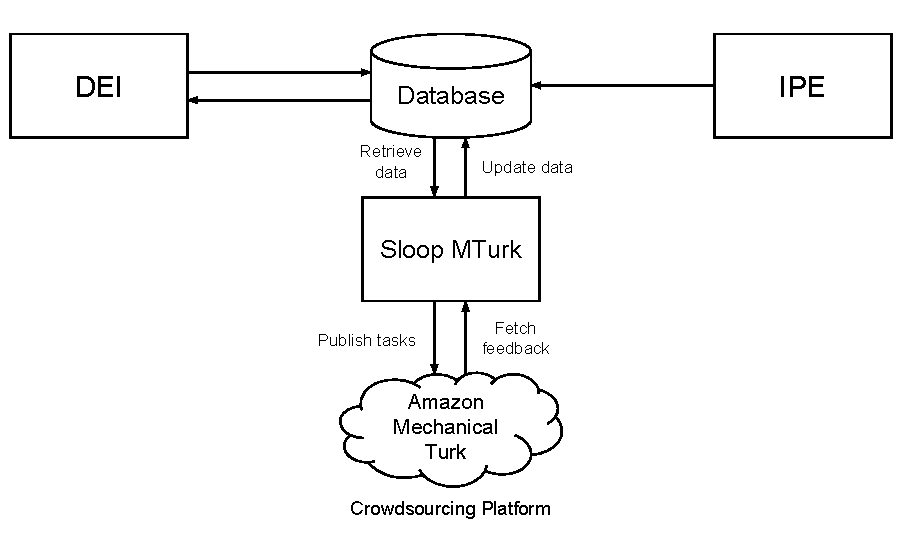
\includegraphics[width=0.8\textwidth]{sloop/turk_system}
    \caption{Sloop Architecture with Sloop MTurk integration}
    \label{fig:turk_overview} %chktex 24
  \end{figure}

  Sloop MTurk communicates with the crowdsourcing platform in order to obtain
  human feedback on the original rankings. Our focus is on

  \subsection{Architecture}

  There are four major functions used within the relevance feedback
  workflow: Retrieve, Publish, Fetch, and Update.

  \subsubsection{Retrieve}

  In the first stage of the relevance feedback workflow, Sloop MTurk retrieves a
  number of known and unknown image pairs from the database in the ratio
  described in Section~\ref{subsub:validation}. The metadata about the retrieved
  pairs, such as the answers to the known pairs, individual identification
  numbers, and source address, is stored in a lightweight SQLite database.

  Sloop MTurk never publishes a duplicated \emph{unknown} pair onto MTurk. It
  actively checks with the local database before any retrieval whether an unknown pair
  has ever been published before. Users can set the sampling policy of Sloop MTurk in
  the configuration file. The default is to use the normal sampling from the
  median whose performance has been shown in
  Chapter~\ref{chap:relevance_feedback}.

  Sloop MTurk only fetches from the Sloop database the images necessary for the
  tasks to be published.  Upon retrieval, Sloop MTurk caches the image data
  locally on the filesystem behind NGINX\@. Caching image data reduces data transfer
  overhead because fetching large responses (like images) over the network is
  both slow and expensive.

  \subsubsection{Publish}

  Sloop MTurk publishes the tasks to MTurk immediately after all the
  information is fetched. The tasks published are available on Amazon Mechanical
  Turk under the title: `Image Matching --- Animals' posted by user `sloop'.
  % TODO Tell user that they need AWS access ID and secret key to
  % programmatically communicate with MTurk

  \subsubsection{Fetch}

  Users can fetch results once the published tasks have been completed. This can
  be run as a cron job.  For each completed task with correct answers to all
  known pairs, Sloop MTurk accepts and retrieves the results, allowing the worker
  to be paid.  For any tasks with incorrect answers to known pairs, Sloop MTurk
  rejects the results, with no payment given.

  Sloop MTurk logs the answers to the unknown pairs from the accepted assignments
  in the local SQLite database. Results are never deleted automatically.

  \subsubsection{Update}

  The update command pushes the answers logged in the local SQLite database back
  to the original Sloop database so that the data is ready for another round of
  relevance feedback. The remote database server then categorizes the captures
  with the data pushed and the existing data, and then performs its cohort
  merging logic~\cite{sloopdocs}.

  The update command is separated from fetch for ease of debugging. In
  practice, we would like to update the upstream database as frequently as
  possible as we have seen in the Experiments section,
  Chapter~\ref{chap:relevance_feedback}.

% section sloop_mturk (end)

% ----------------------------

% Adaptive sampling method
% Methodology
% * Design and Architecture
% * Population of interest and sampling subject used in the study
% * Instrument and what it measures (metrices)
% * qualifications of informants if used in the study
% * Validation
% * Data gathering procedure (experiments)
\graphicspath{{./images/chap6/}}
% Adaptive sampling method
% Methodology
% * Design and Architecture
% * Population of interest and sampling subject used in the study
% * Instrument and what it measures (metrics)
% * qualifications of informants if used in the study
% * Validation
% * Data gathering procedure (experiments)
\chapter{Relevance Feedback with Adaptive Sampling}

One of the most important questions we would like to answer is: given an
initial distribution of scores, where should we be sampling from? In this
chapter, we take advantage from the fact that we gradually gain more
information about the score distribution over time to dynamically determine
where we should be sampling from.

First, we perform different statistical analyses on the data. Then we propose a
new sampling scheme based on our analyses. Finally, we set up an experiment to
compare the performance of our proposed scheme to the other standard sampling
policies we have implemented.

\section{Statistical Analysis}

\subsection{Probability of Score given matches/non-matches}

We can estimate the probability of score given a match by
$$\Pr{(score=s \mid match)} = \frac{\texttt{\# matches\_whose\_score=s}}
    {\texttt{\# matches}}$$
In the same way,
$$\Pr{(score=s \mid nonmatch)} = \frac{\texttt{\# nonmatches\_whose\_score=s}}
    {\texttt{\# nonmatches}}$$

\begin{figure}[htbp]
  \centering
  \begin{subfigure}[t]{\textwidth}
    \centering
    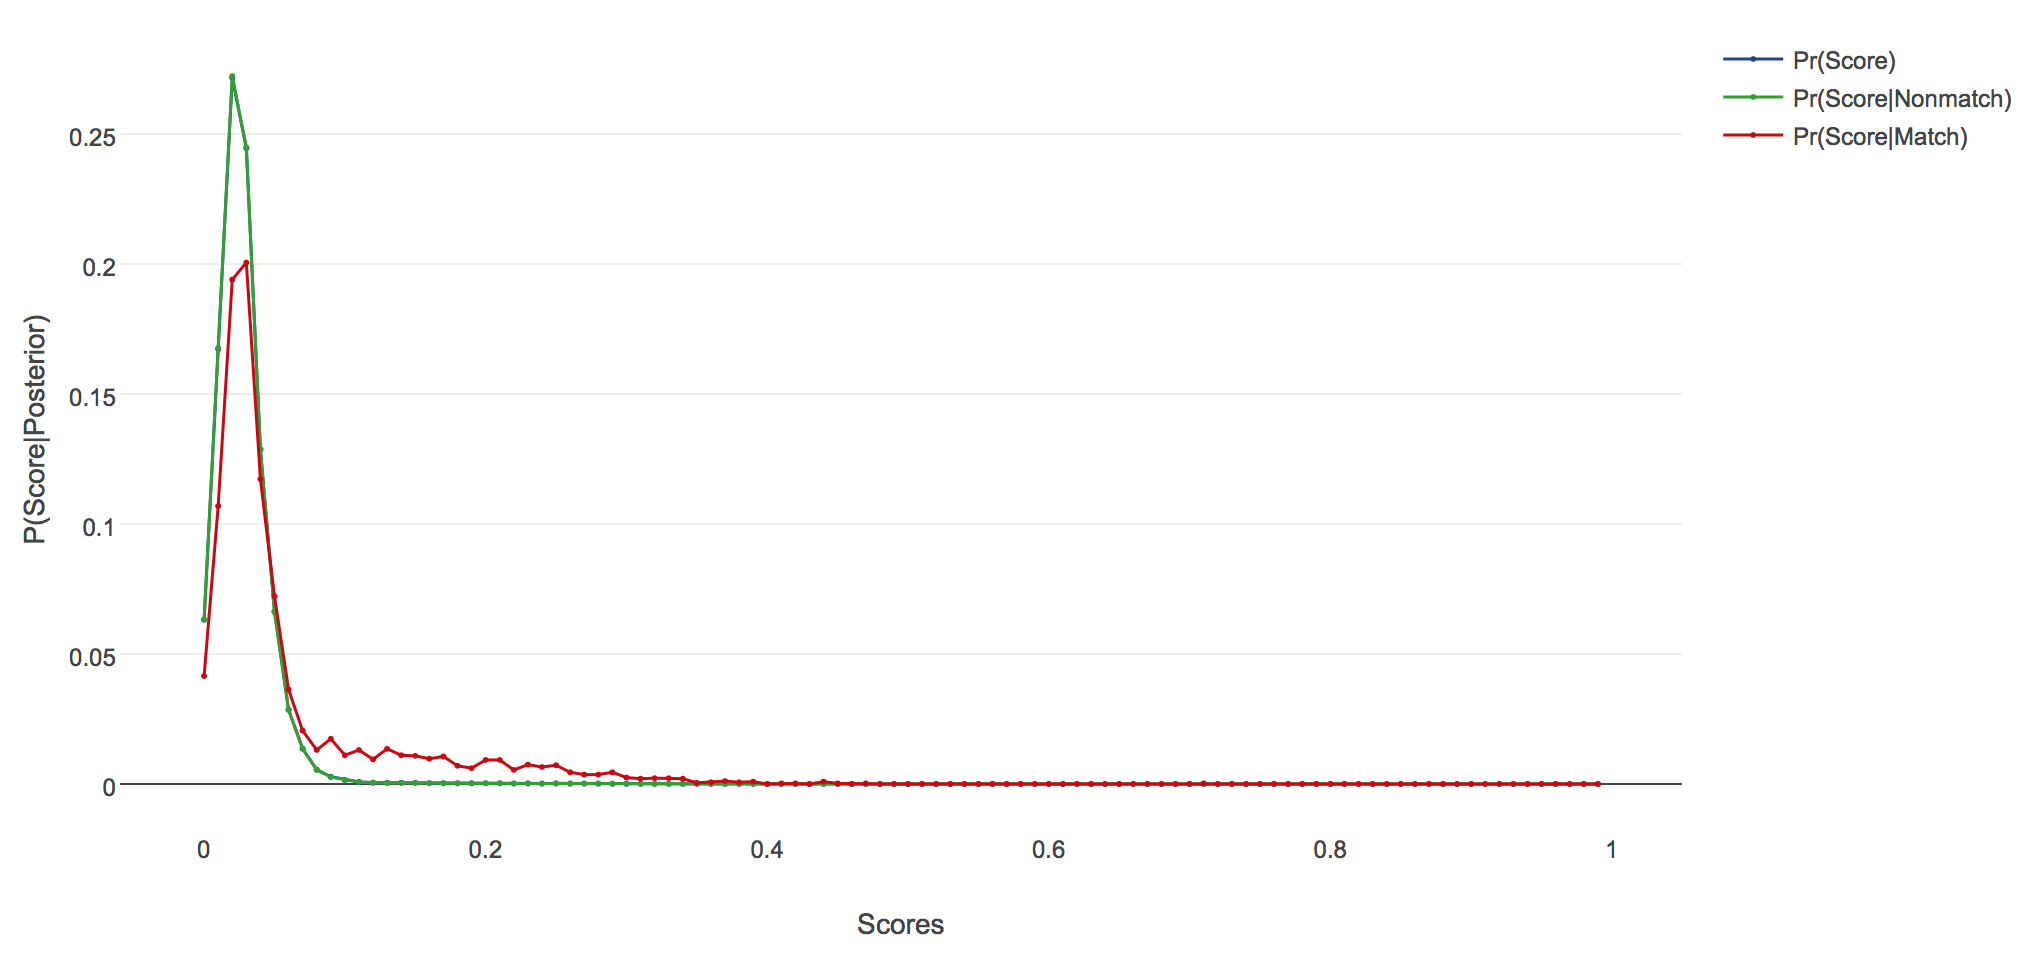
\includegraphics[width=0.8\textwidth]{dataset/grand/psm}
    \caption{Probability of Score given matches/non-matches}
    \label{fig:grand_psm} %chktex 24
  \end{subfigure}%

  \begin{subfigure}[t]{\textwidth}
    \centering
    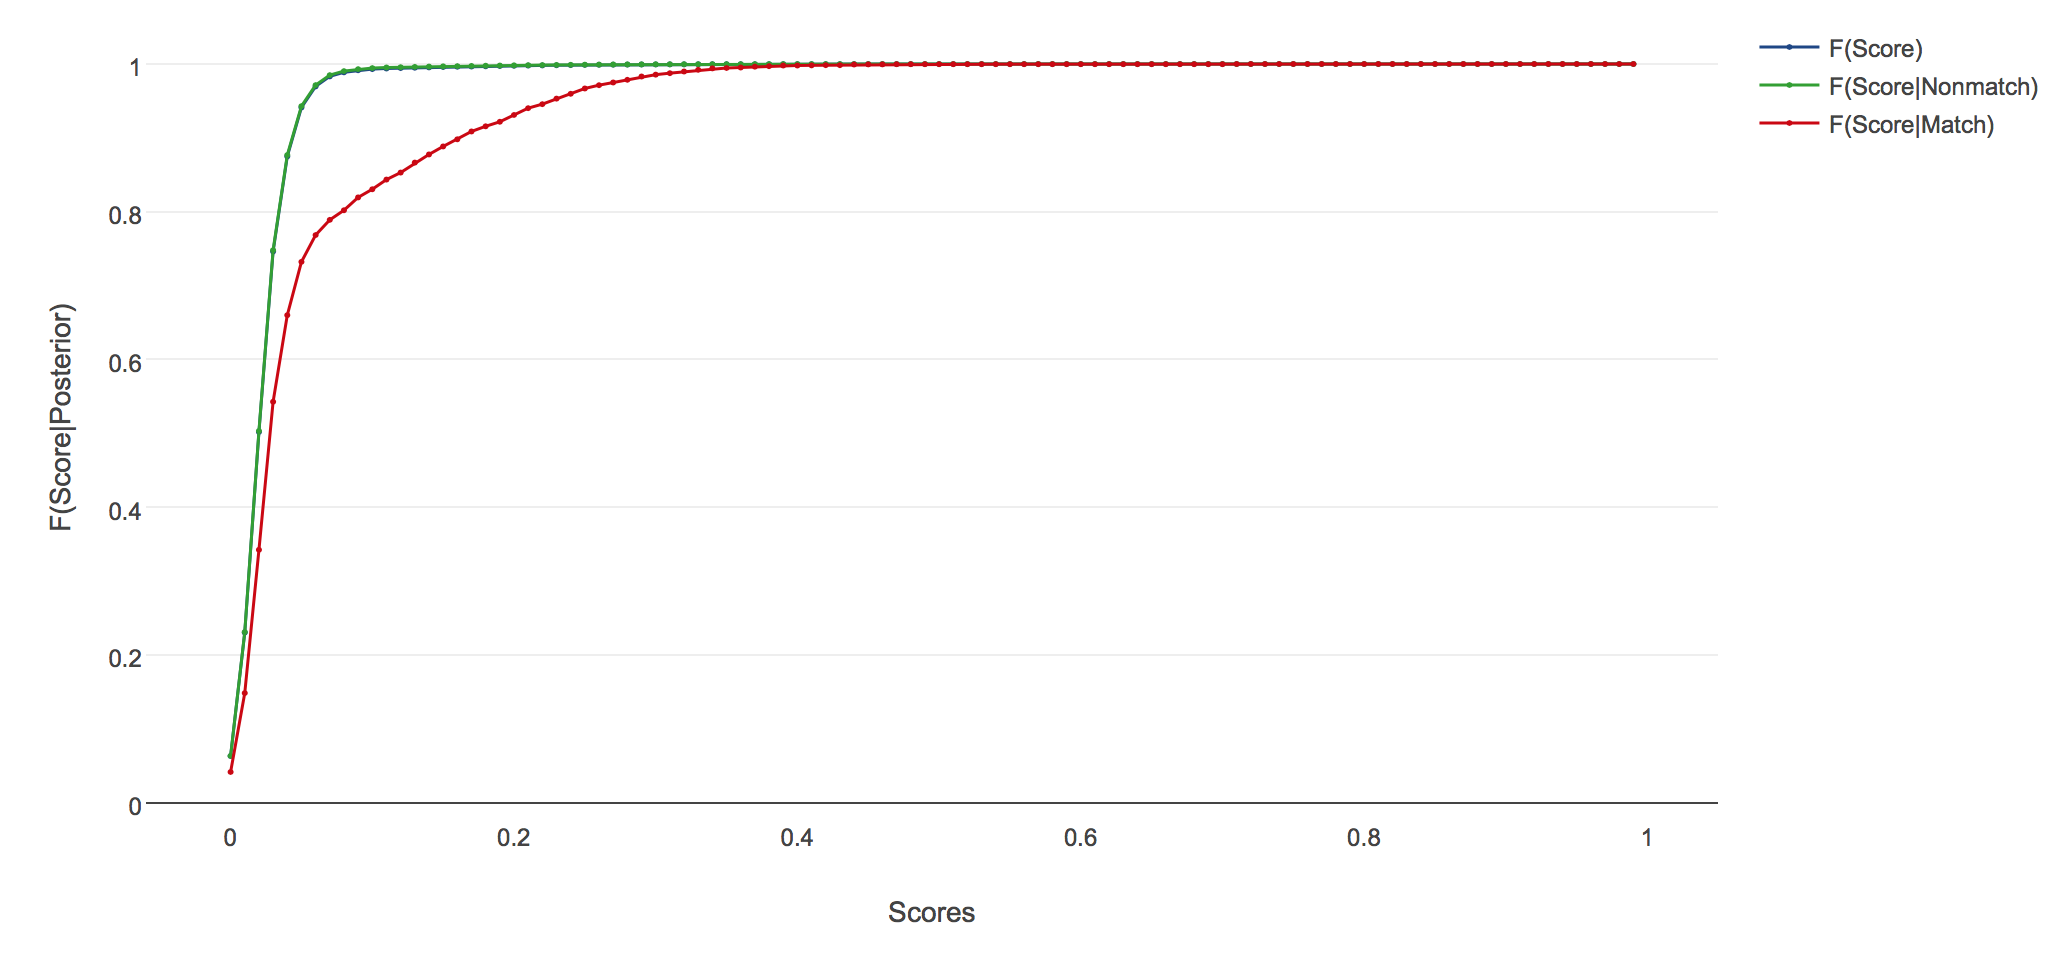
\includegraphics[width=0.8\textwidth]{dataset/grand/csm}
    \caption{CDF of Score given matches/non-matches}
    \label{fig:grand_csm} %chktex 24
  \end{subfigure}%

  \begin{subfigure}[t]{\textwidth}
    \centering
    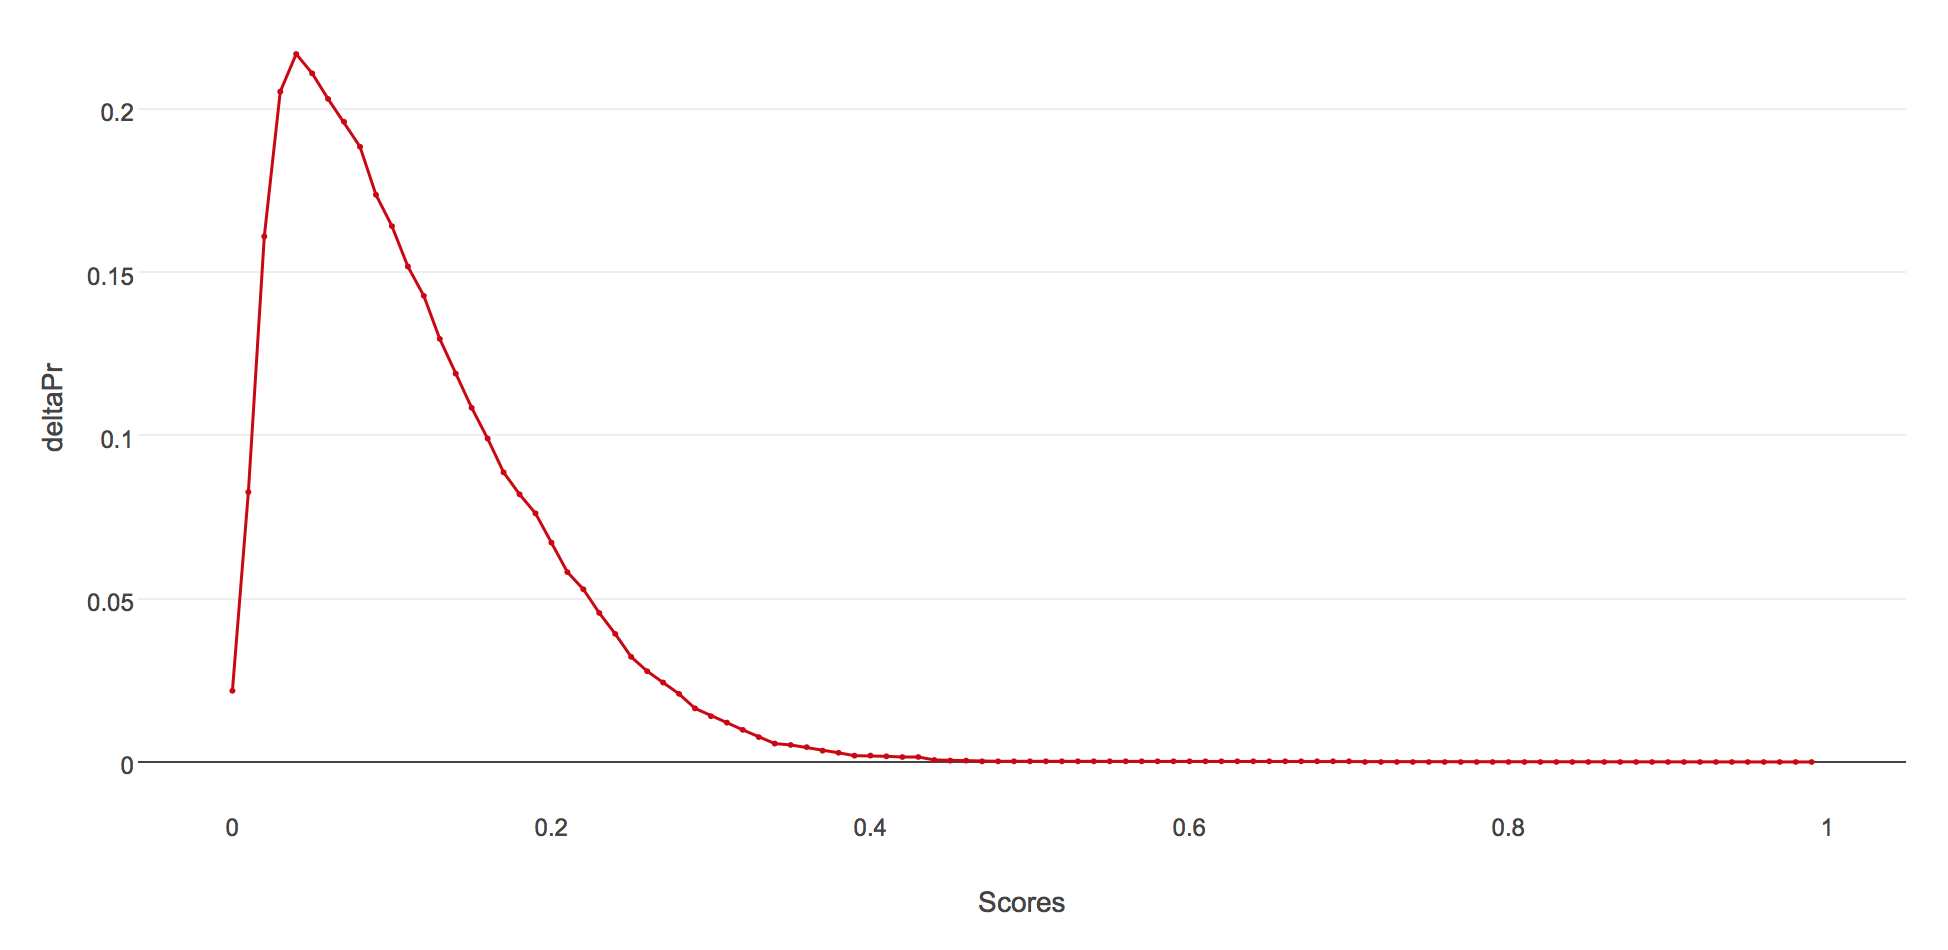
\includegraphics[width=0.8\textwidth]{dataset/grand/dsm}
    \caption{Difference between the CDF of Score given matches/non-matches}
    %$F\[non-match\]$ and $F\[match\]$
  \end{subfigure}%
  \caption{Grand}
  \label{fig:grand_sm} %chktex 24
\end{figure}

From Figure~\ref{fig:grand_sm}, we can deduct following conclusions:
\begin{itemize}
\item Most of the cohorts has score between 0 and 0.07 overall so most matches
and non-matches have score less than 0.06.
\item We expected $\Pr{(score \mid match)}$ to increase as the function of score
, but it turns out that it actually decreases. This results from the fact that
there are \emph{very few} matches with scores higher than 0.33, which is the 99th
percentile of the matches' score.
\item The number of matches with $score \in [0.08, 0.35)$ is greater than that of
non-matches with the score in the same range. That is
$$\Pr{(score \mid match)} > \Pr{(score \mid nonmatch)} \mbox{ where } score\in [0.08, 0.35)$$
\end{itemize}

\begin{figure}[htbp]
  \centering
  \begin{subfigure}[t]{\textwidth}
      \centering
      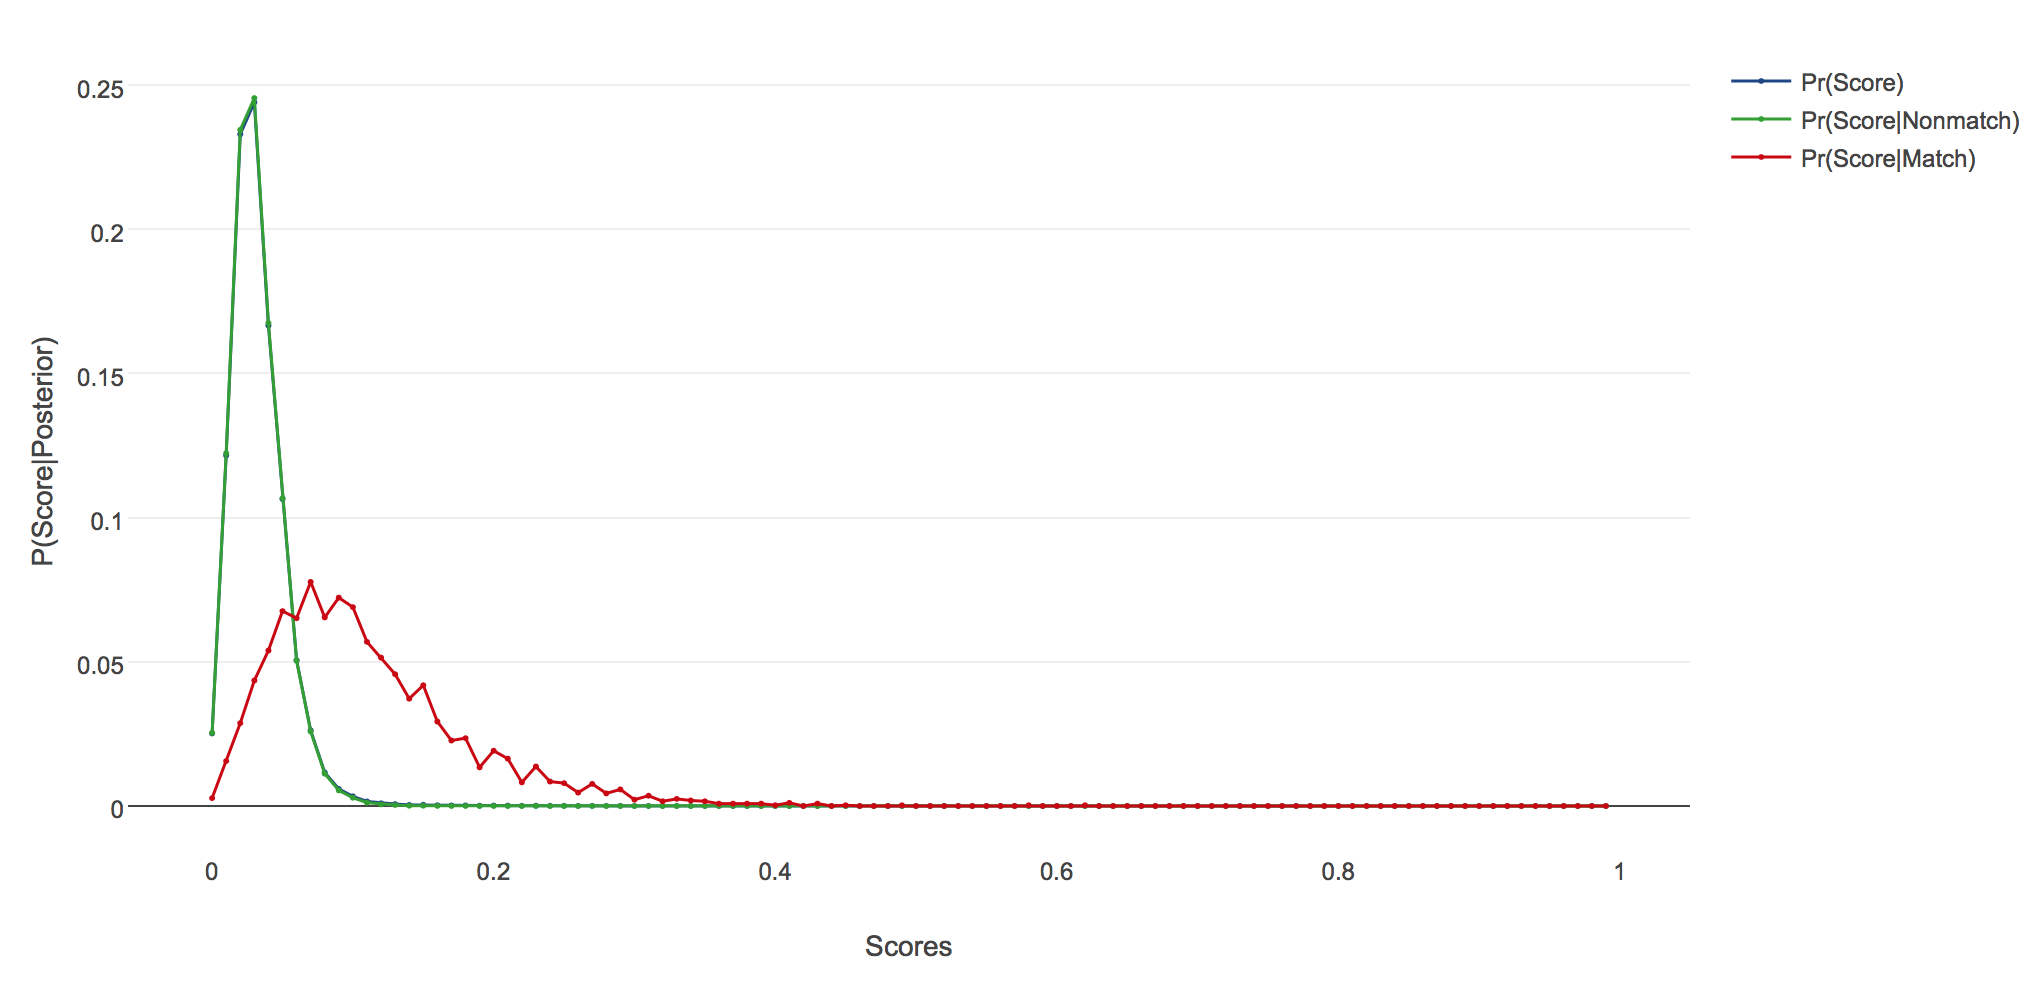
\includegraphics[width=0.8\textwidth]{dataset/otago/psm}
        \caption{Probability of Score given matches/non-matches}
      \label{fig:otago_psm} %chktex 24
    \end{subfigure}%
  \\
  \begin{subfigure}[t]{\textwidth}
      \centering
      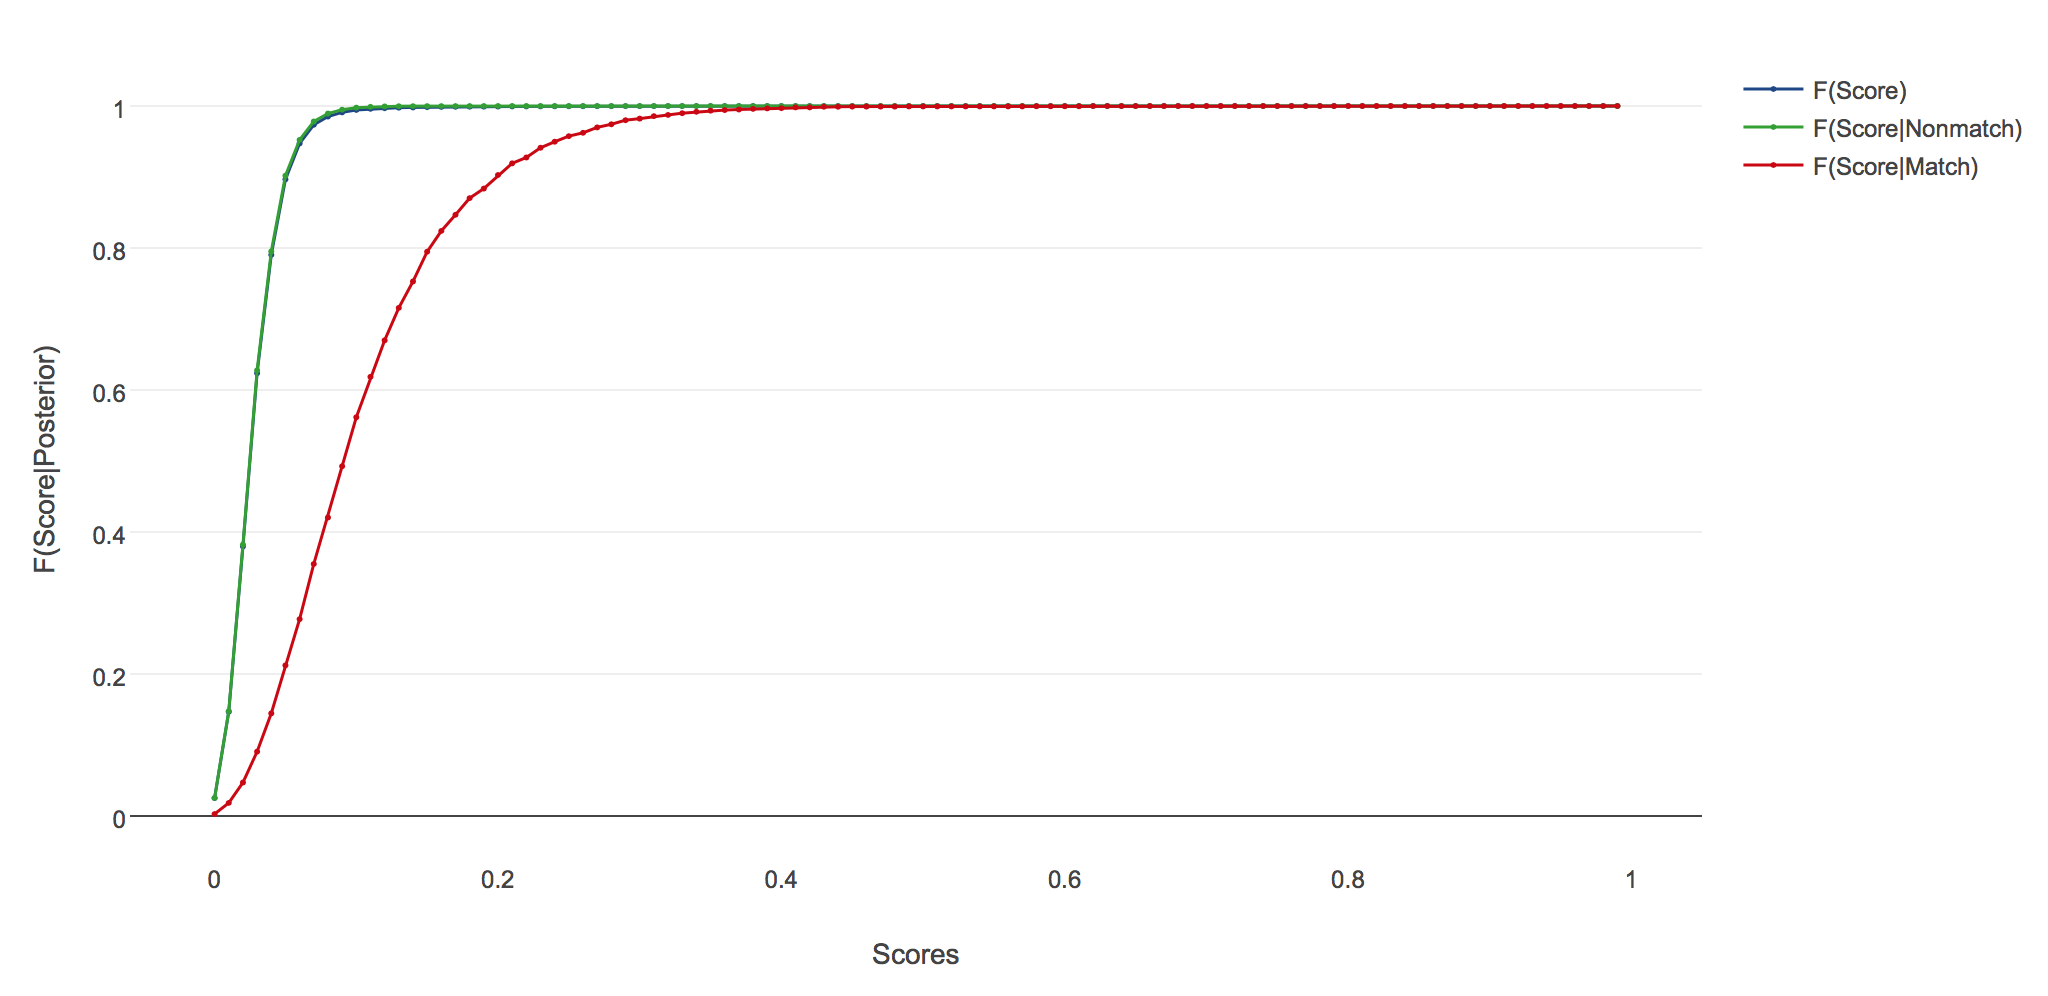
\includegraphics[width=0.8\textwidth]{dataset/otago/csm}
        \caption{CDF of Score given matches/non-matches}
      \label{fig:otago_csm} %chktex 24
    \end{subfigure}%
  \\
  \begin{subfigure}[t]{\textwidth}
      \centering
      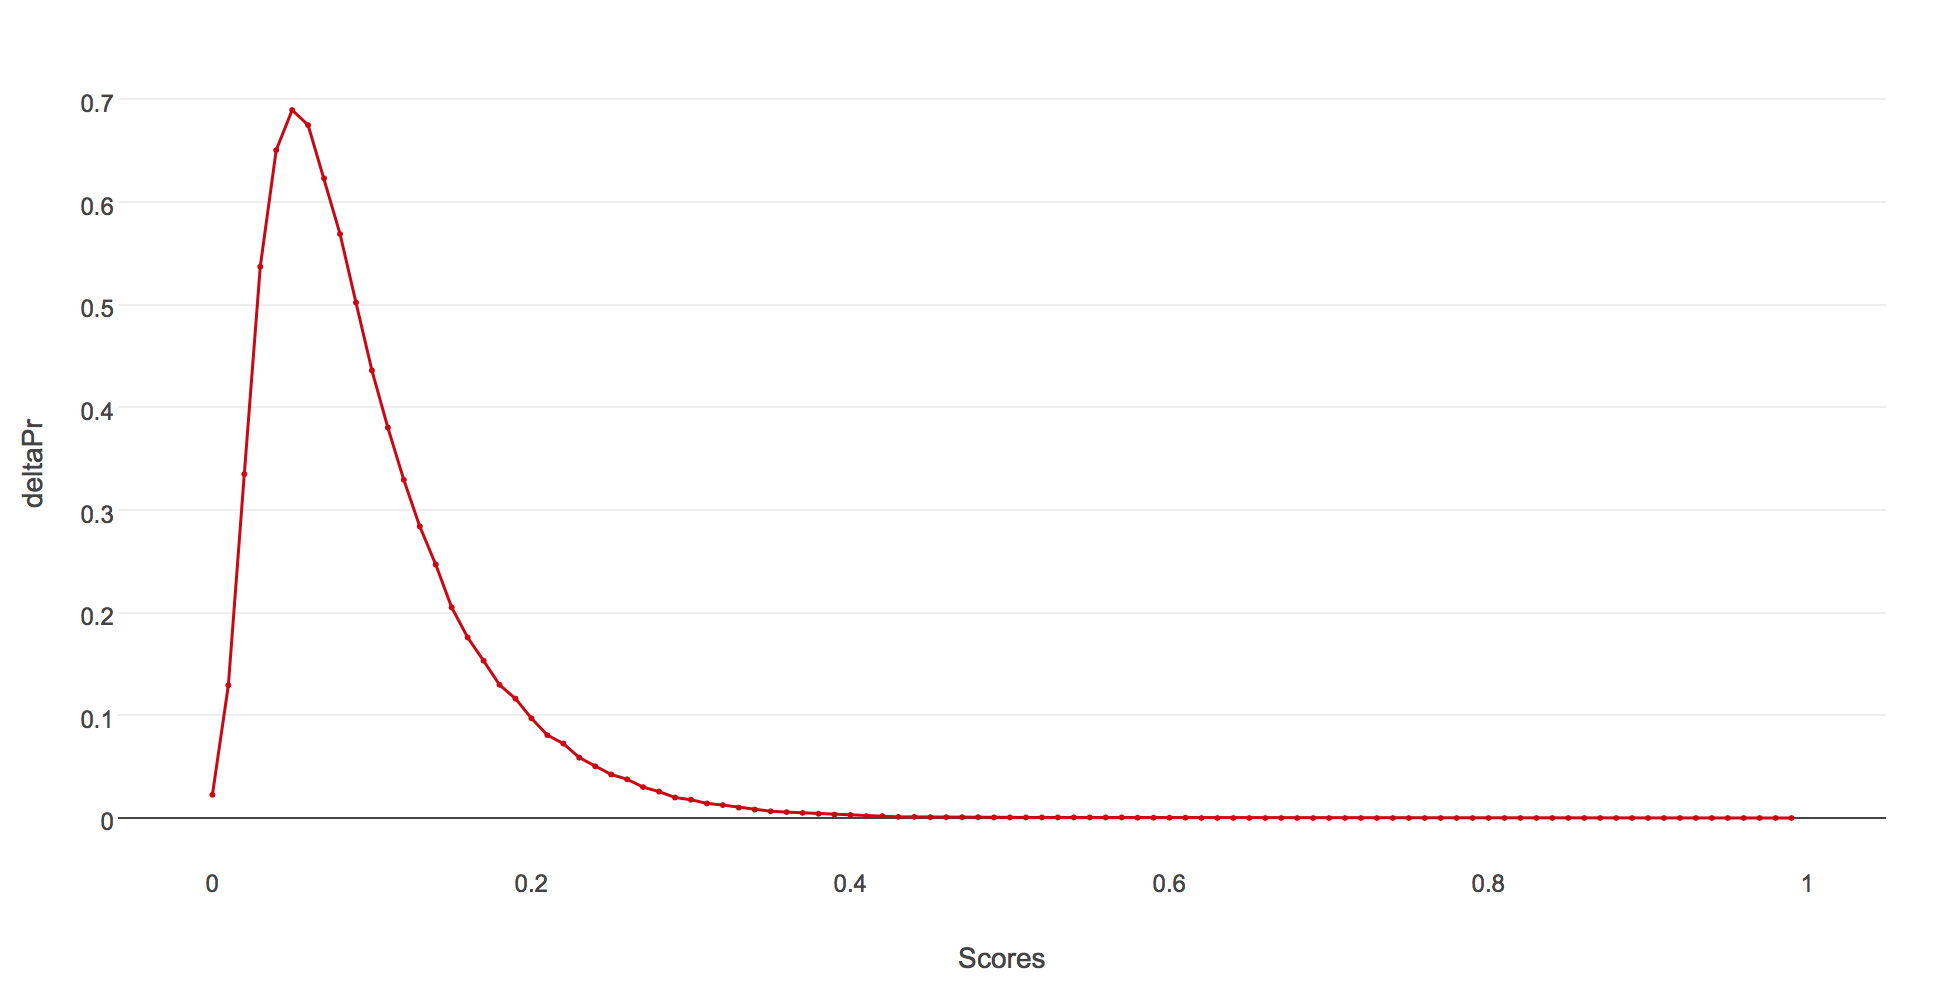
\includegraphics[width=0.8\textwidth]{dataset/otago/dsm}
        \caption{Difference between the CDF of Score given matches/non-matches}
        \label{fig:otago_dsm} %chktex 24
    %$F\[non-match\]$ and $F\[match\]$
    \end{subfigure}%
  \caption{Functions of Score given matches/non-matches}
  \label{fig:otago_sm}
\end{figure}

% TODO analyze Otago

\subsection{Probability of a matching score at a given cohort size}

\begin{figure}[htbp]
    \centering
    \begin{subfigure}[t]{\textwidth}
        \centering
        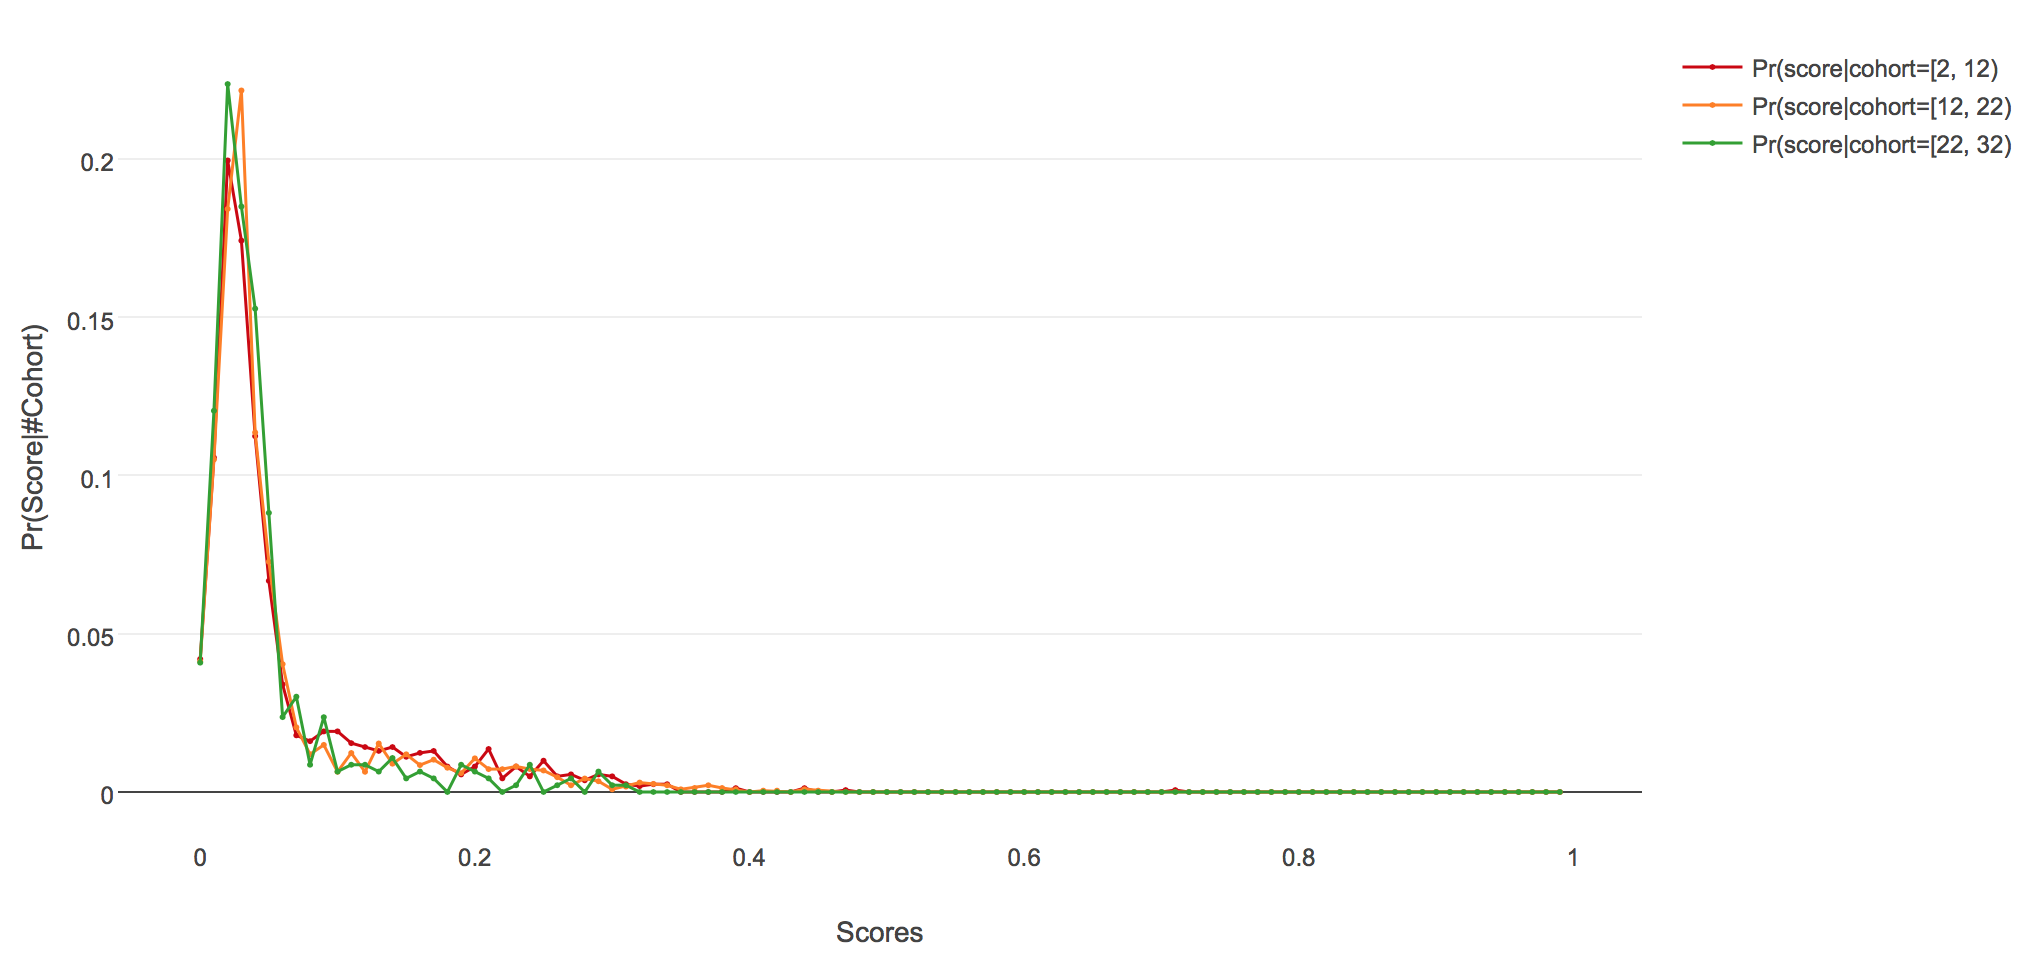
\includegraphics[width=0.8\textwidth]{dataset/grand/pscohort}
        \caption{Probability of a matching score at a given cohort size}
        \label{fig:grand_pscohort} %chktex 24
    \end{subfigure}%
    \\
    \begin{subfigure}[t]{\textwidth}
        \centering
        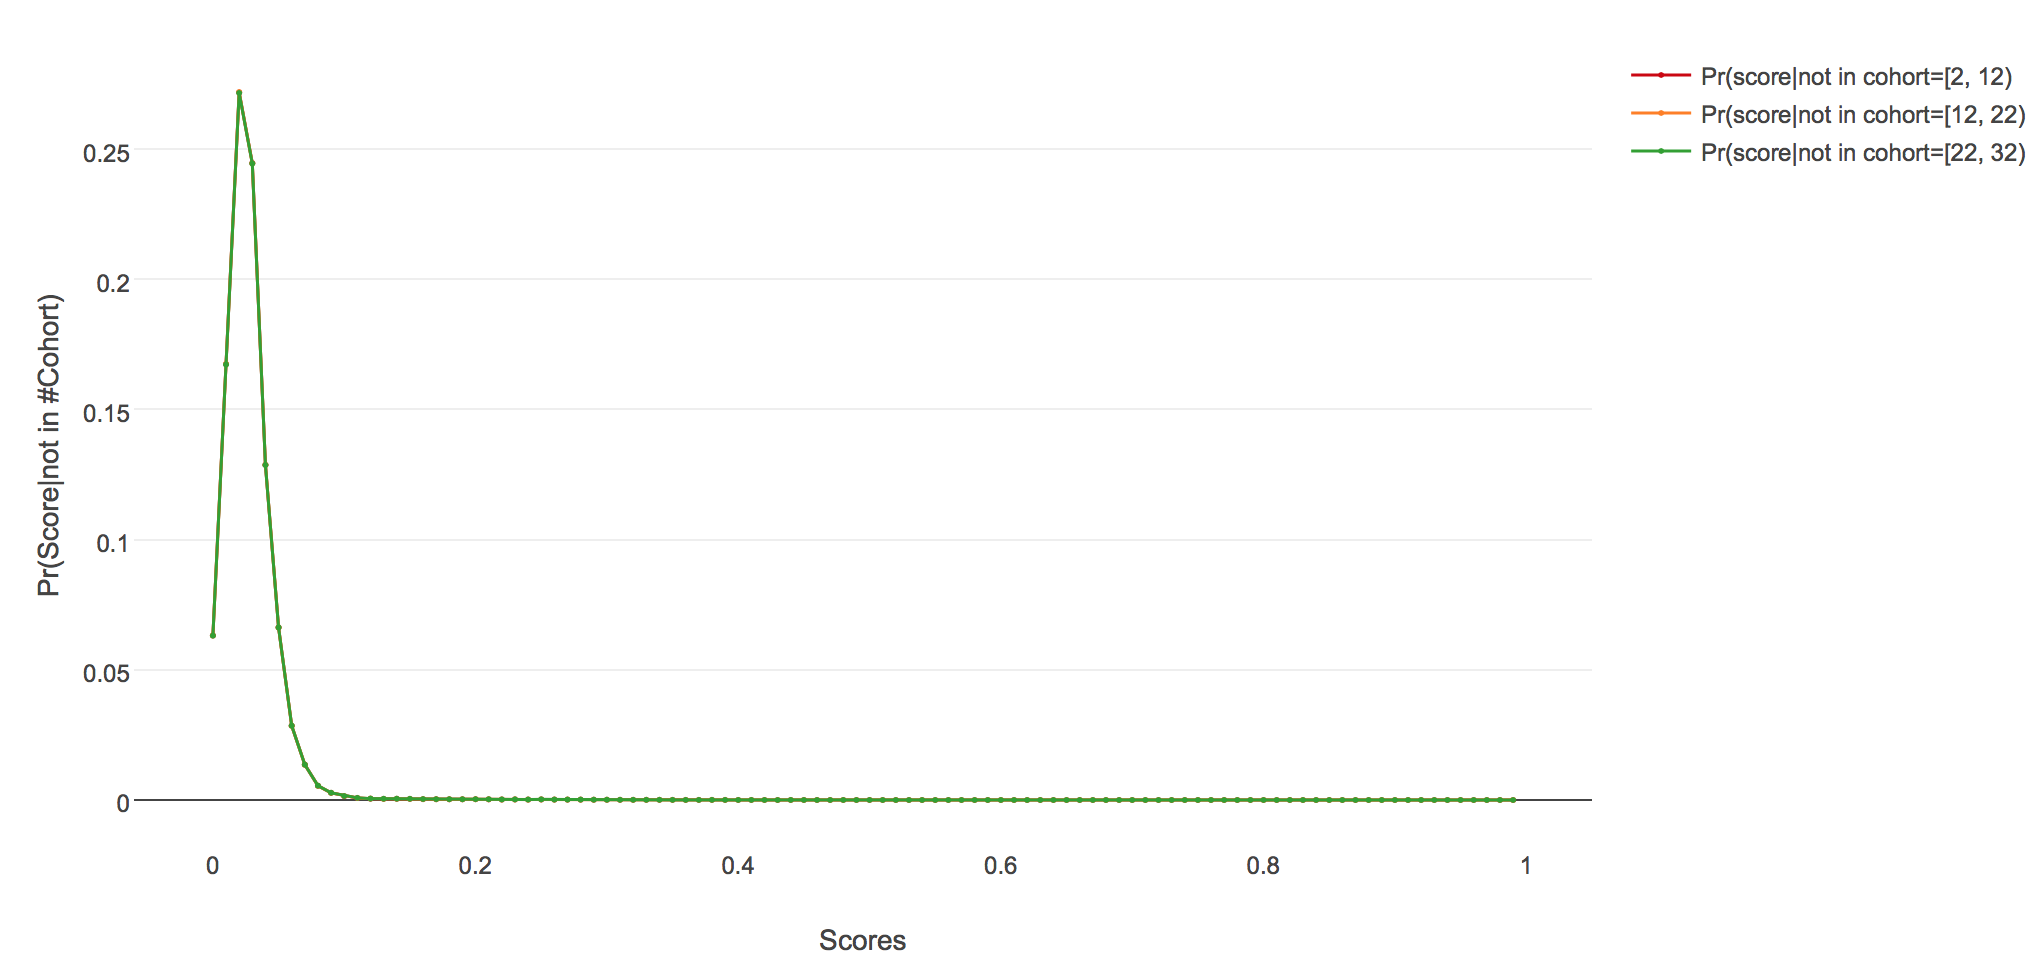
\includegraphics[width=0.8\textwidth]{dataset/grand/psnoncohort}
        \caption{Probability of a score \emph{not} in a given cohort size}
        \label{fig:grand_psnoncohort} %chktex 24
    \end{subfigure}%
    \caption{Grand}
    \label{fig:grand_psc} %chktex 24
\end{figure}

Initially, we expected that as the cohort size increases, $\Pr{(score \mid
\#cohort)}$ should peak closer to 1 since $\texttt{selfscore}$ should decrease
and $\max{(\texttt{sift\_match}(I_i, I_j))}$ should increase as the number of
captures in a cohort increases. However, the distribution of $\Pr{(score \mid
\#cohort)}$ for all numbers of cohorts seem to be similar to one another.

\begin{figure}[htbp]
    \centering
    \begin{subfigure}[t]{\textwidth}
        \centering
        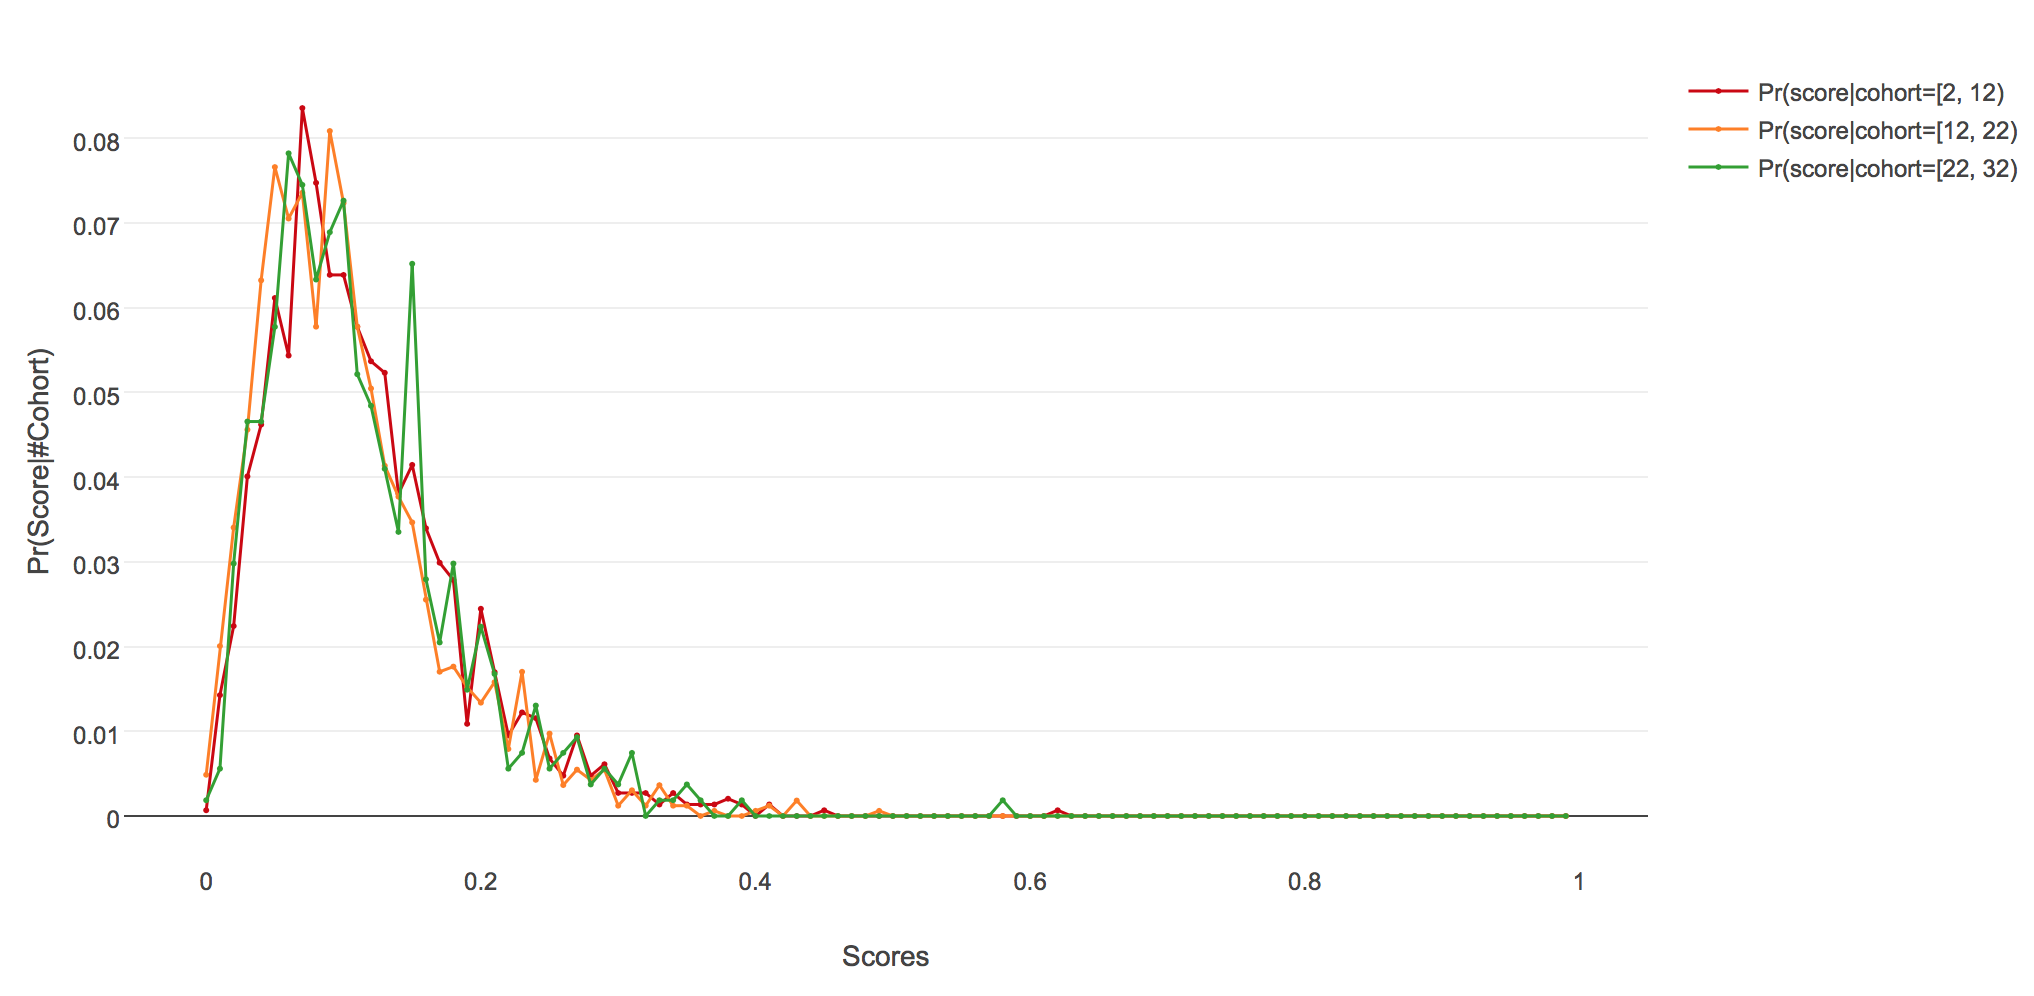
\includegraphics[width=0.8\textwidth]{dataset/otago/pscohort}
        \caption{Probability of a matching score at a given cohort size}
        \label{fig:otago_pscohort} %chktex 24
    \end{subfigure}%
    \\
    \begin{subfigure}[t]{\textwidth}
        \centering
        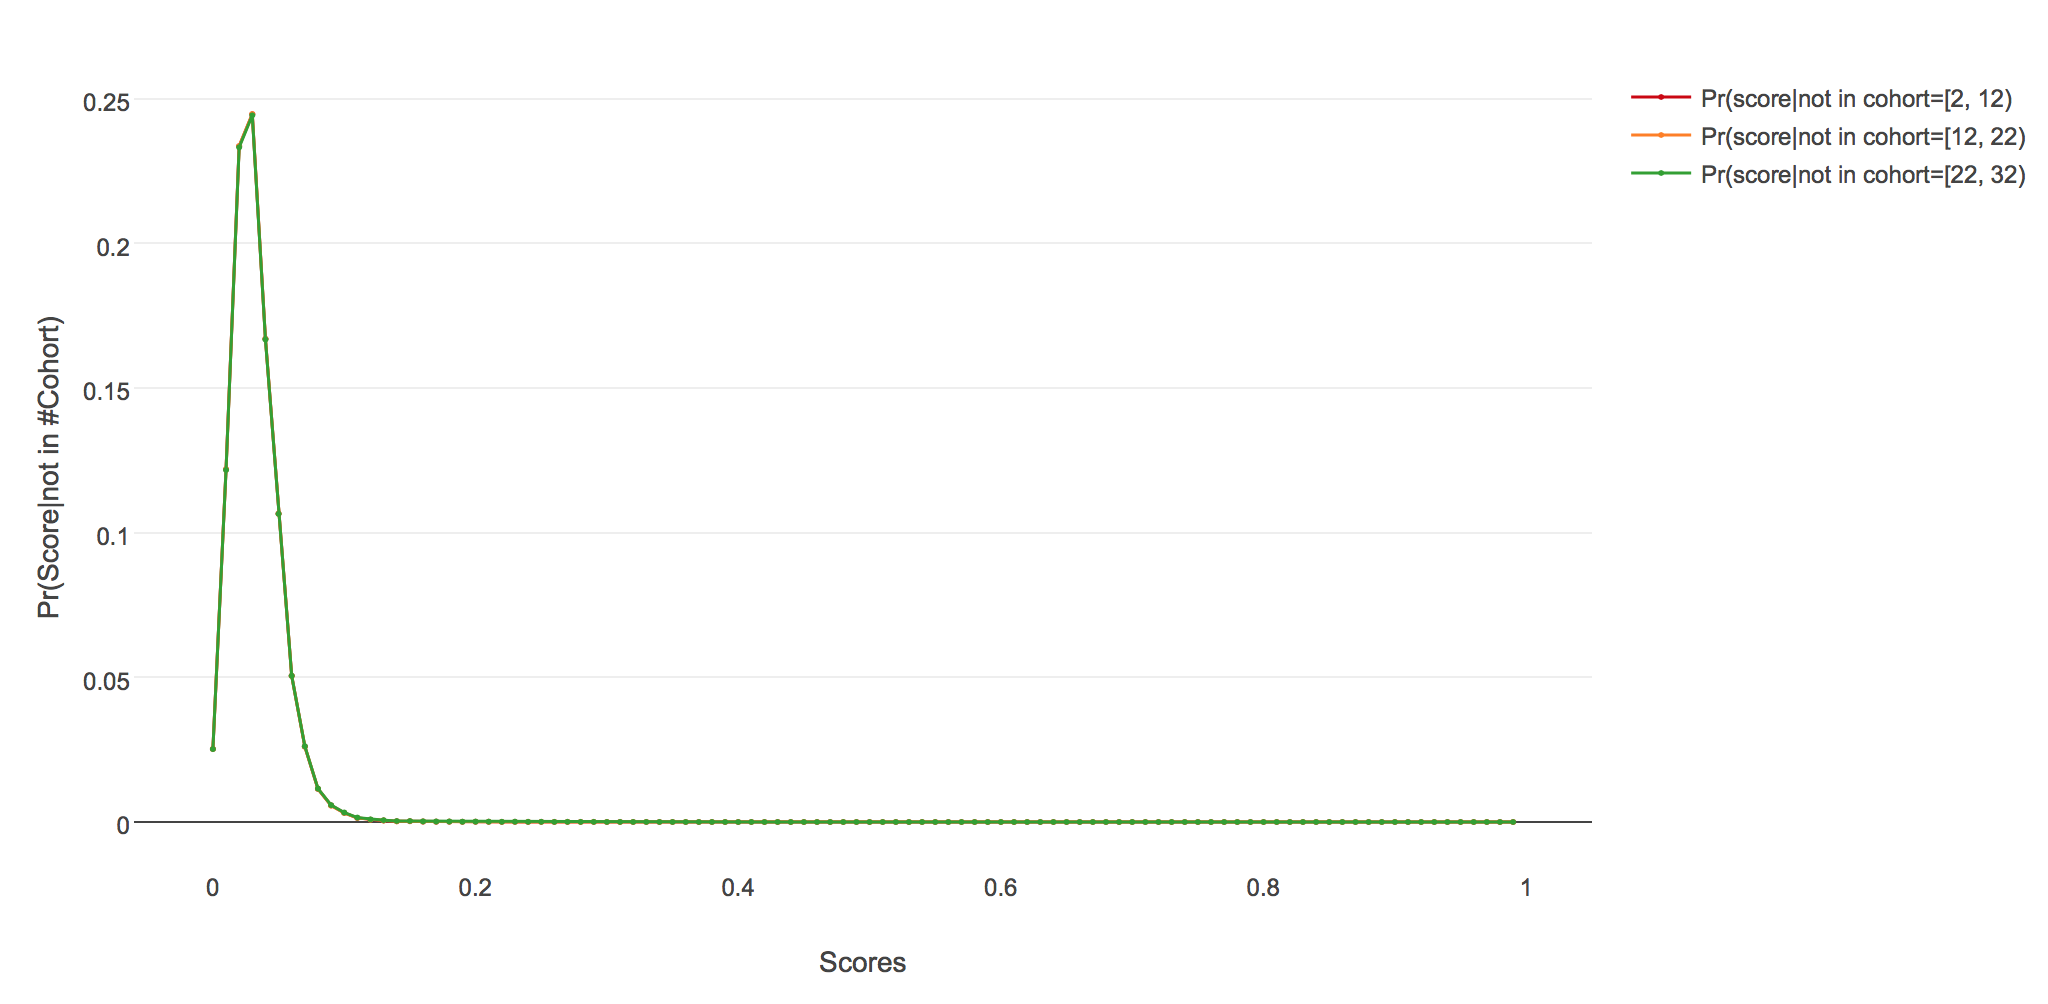
\includegraphics[width=0.8\textwidth]{dataset/otago/psnoncohort}
        \caption{Probability of a score \emph{not} in a given cohort size}
        \label{fig:otago_psnoncohort} %chktex 24
    \end{subfigure}%
    \caption{Otago}
    \label{fig:otago_psc} %chktex 24
\end{figure}

\FloatBarrier%
\subsection{Earth Mover's Distance}

We use Earth Mover's Distance (EMD)~\cite{emd00} as our metric to calculate the
minimal cost required to transform $\Pr{(score \mid nonmatch)}$ to $\Pr{(score \mid match)}$.


Initially, we also expected that the relationship between EMD and cohort size
should be Gaussian. However, there seem to be no relationship between
$\Pr{(score \mid nonmatch)}$ and $\Pr{(score \mid match)}$.


\begin{figure}[htbp]
  \centering
  \begin{subfigure}[t]{\textwidth}
    \centering
    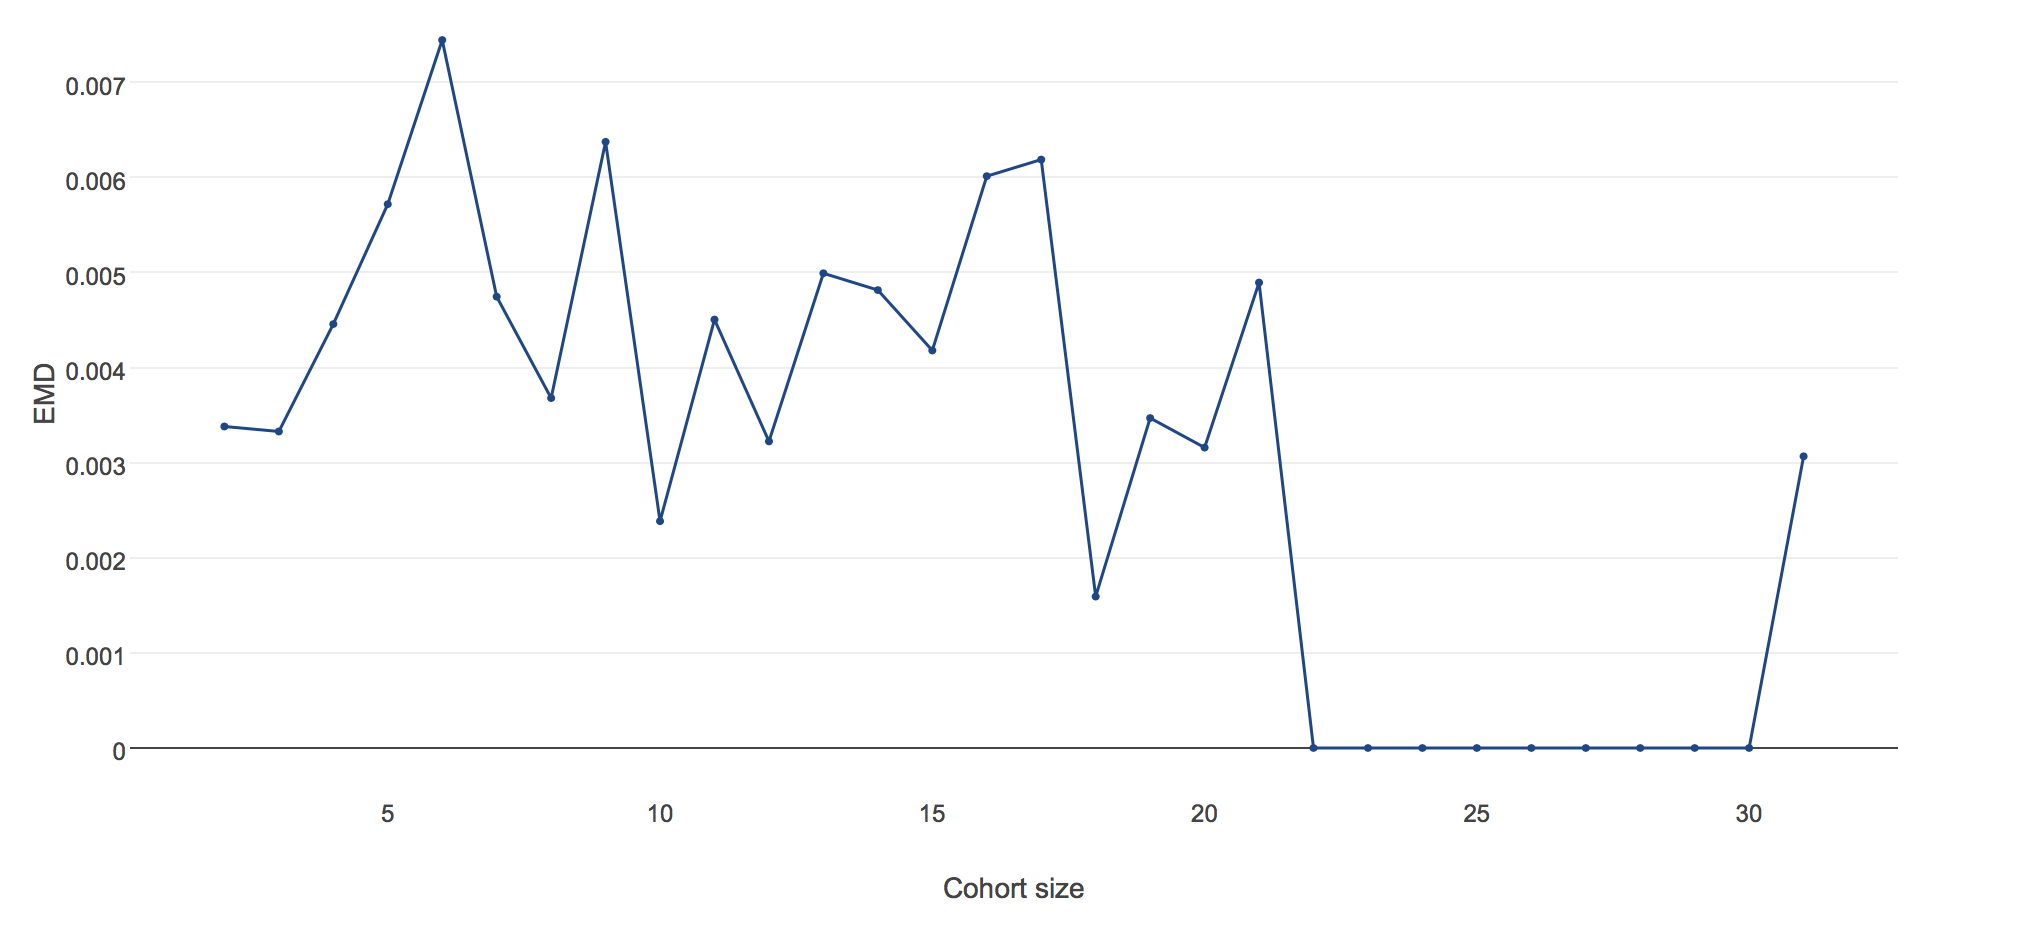
\includegraphics[width=0.8\textwidth]{dataset/grand/emd}
    \caption{Grand}
    \label{fig:grand_emd} %chktex 24
  \end{subfigure}%
  \\
  \begin{subfigure}[t]{\textwidth}
    \centering
    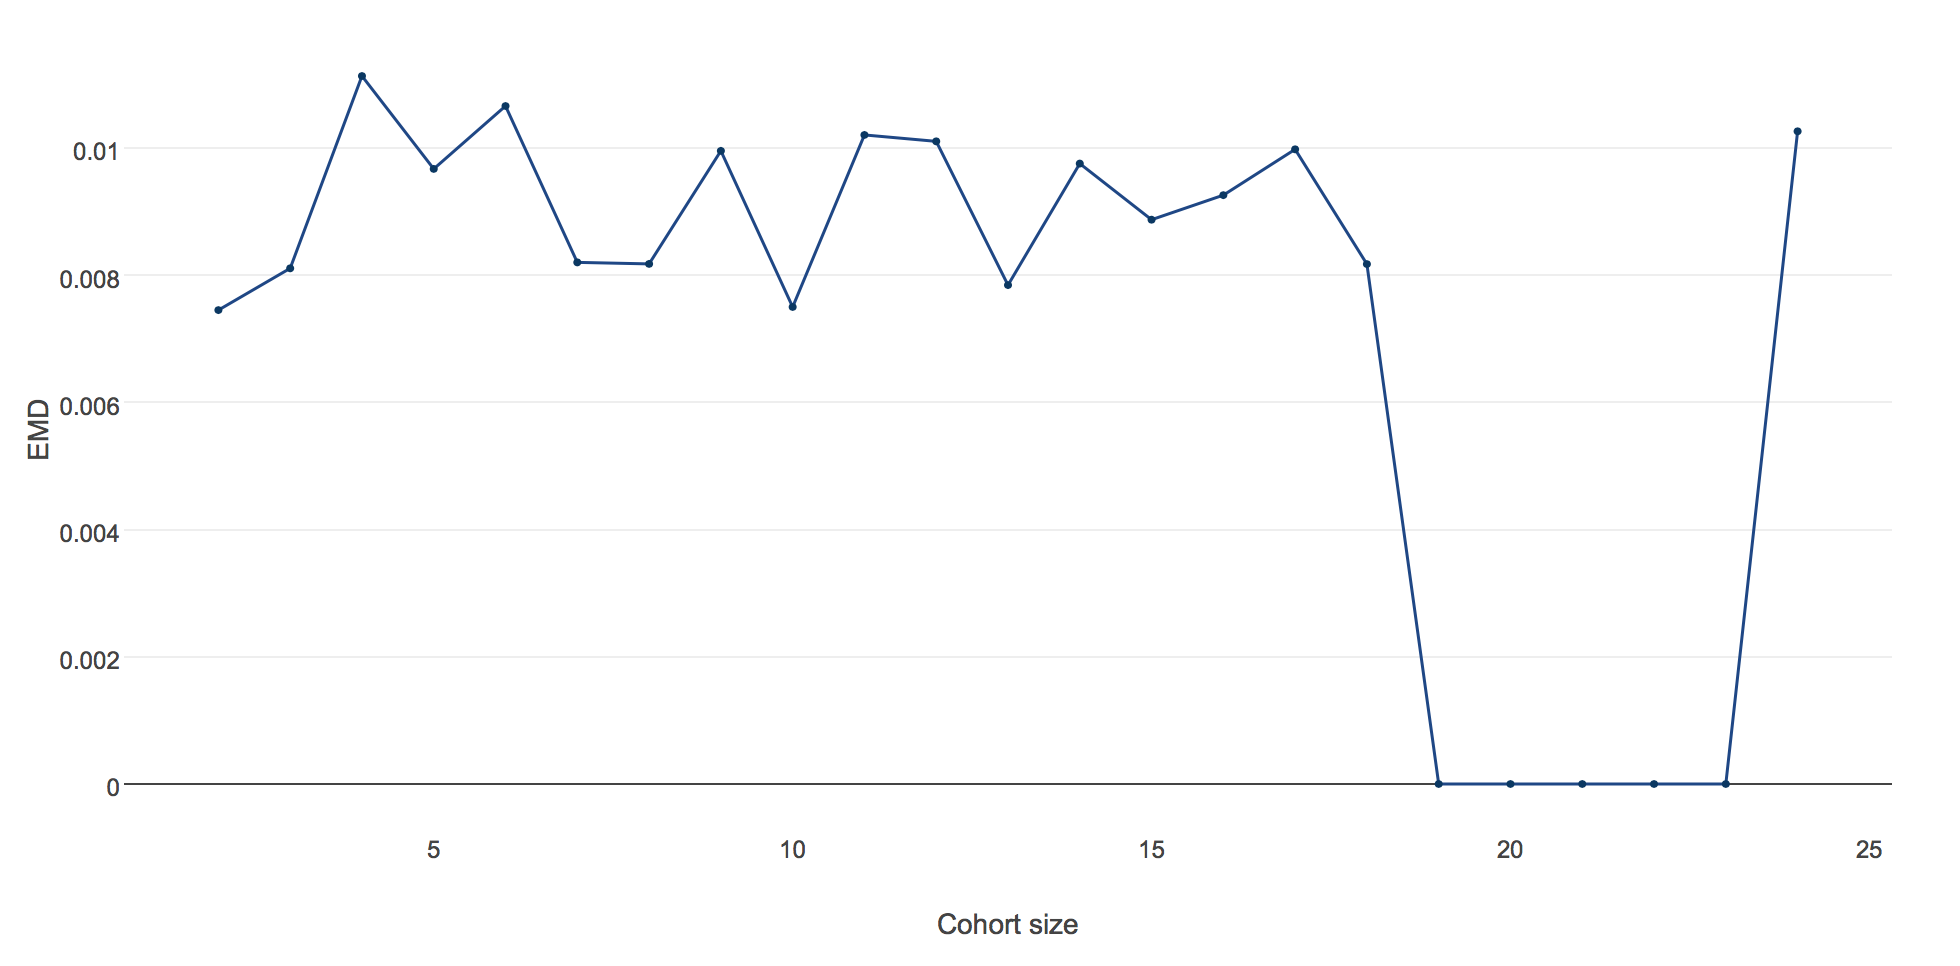
\includegraphics[width=0.8\textwidth]{dataset/otago/emd}
    \caption{Otago}
    \label{fig:otago_emd} %chktex 24
  \end{subfigure}%
  \caption{Earth Mover's Distance between the probability distributions}
  \label{fig:emdist} %chktex 24
\end{figure}

\subsection{Entropy of $\Pr{(score \mid match)}$ at different cohort sizes}

Entropy is the average amount of information we get from each distribution.
$H(X|Y)$ = amount of randomness in the random variable X given the event Y.

\begin{figure}[htbp]
    \centering
    \begin{subfigure}[t]{\textwidth}
        \centering
        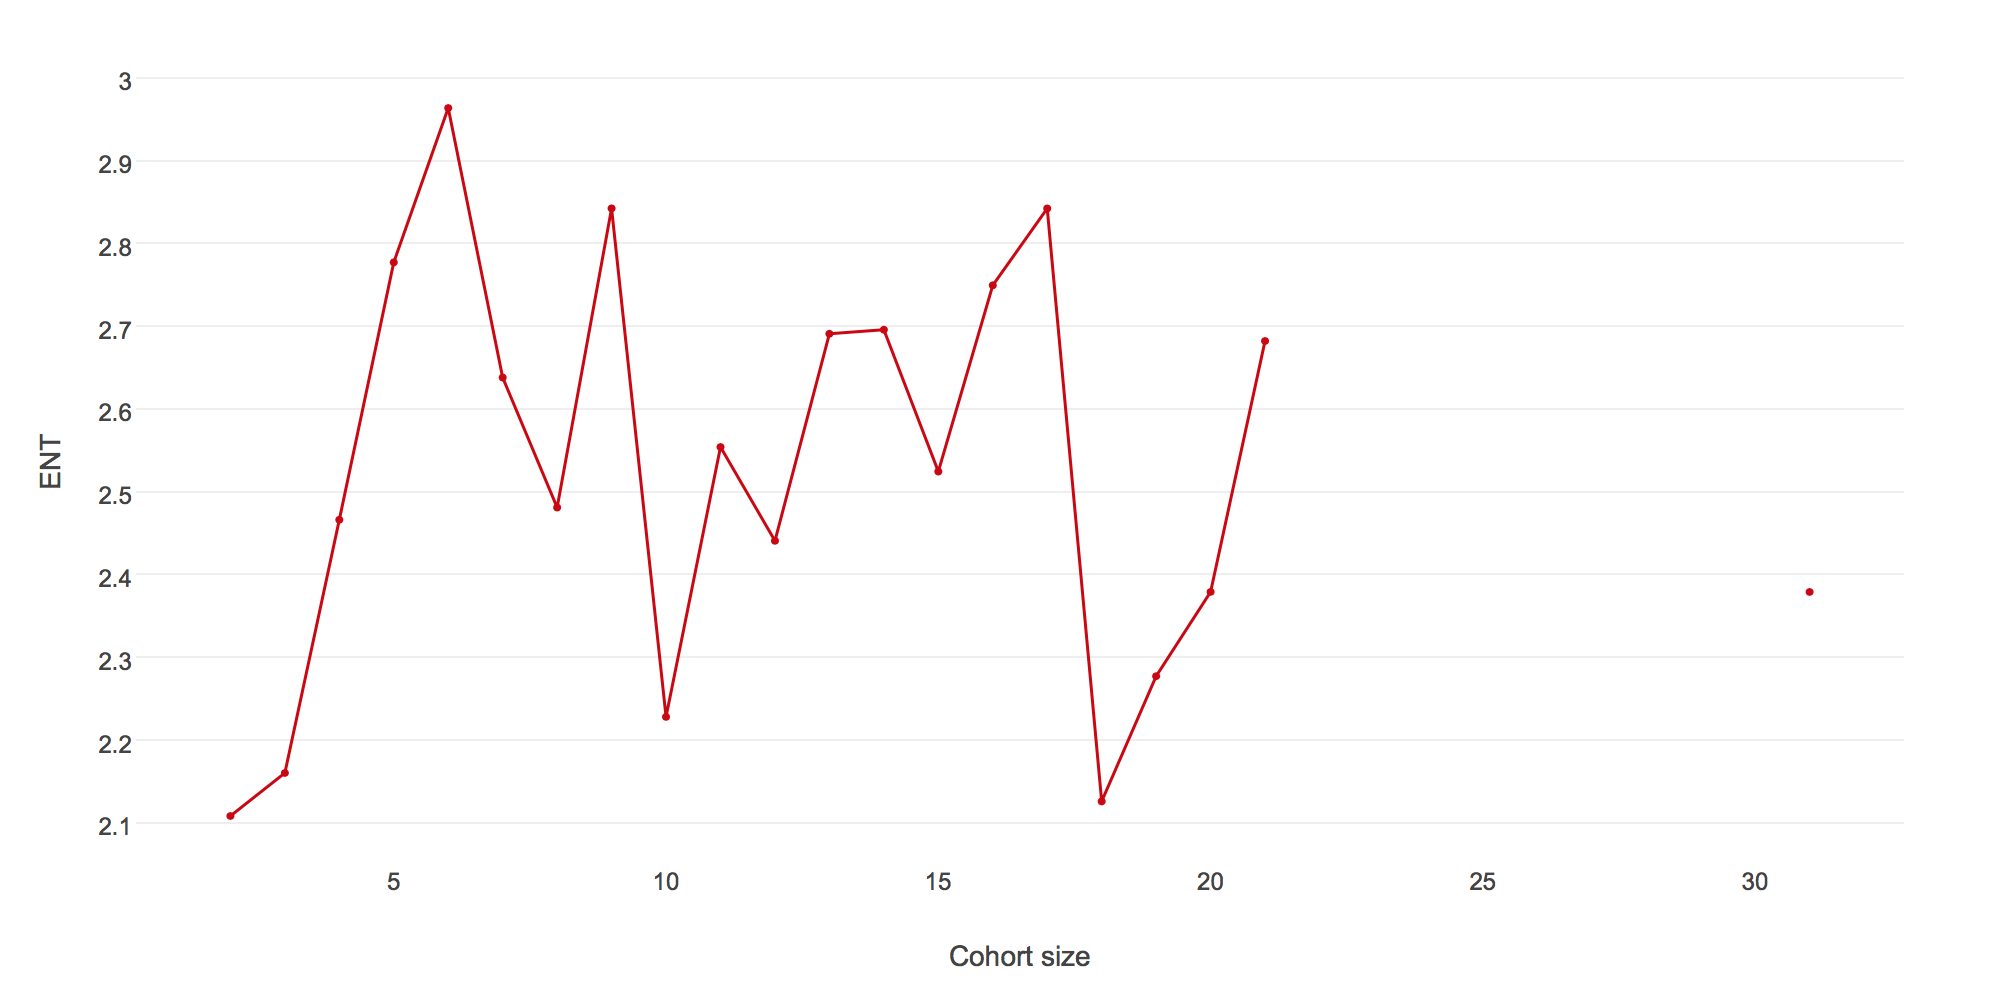
\includegraphics[width=0.8\textwidth]{dataset/grand/ent_psm}
        \caption{Entropy of $\Pr{(score \mid match)}$ at different cohort sizes}
        \label{fig:grand_ent_psm} %chktex 24
    \end{subfigure}%
    \\
    \begin{subfigure}[t]{\textwidth}
        \centering
        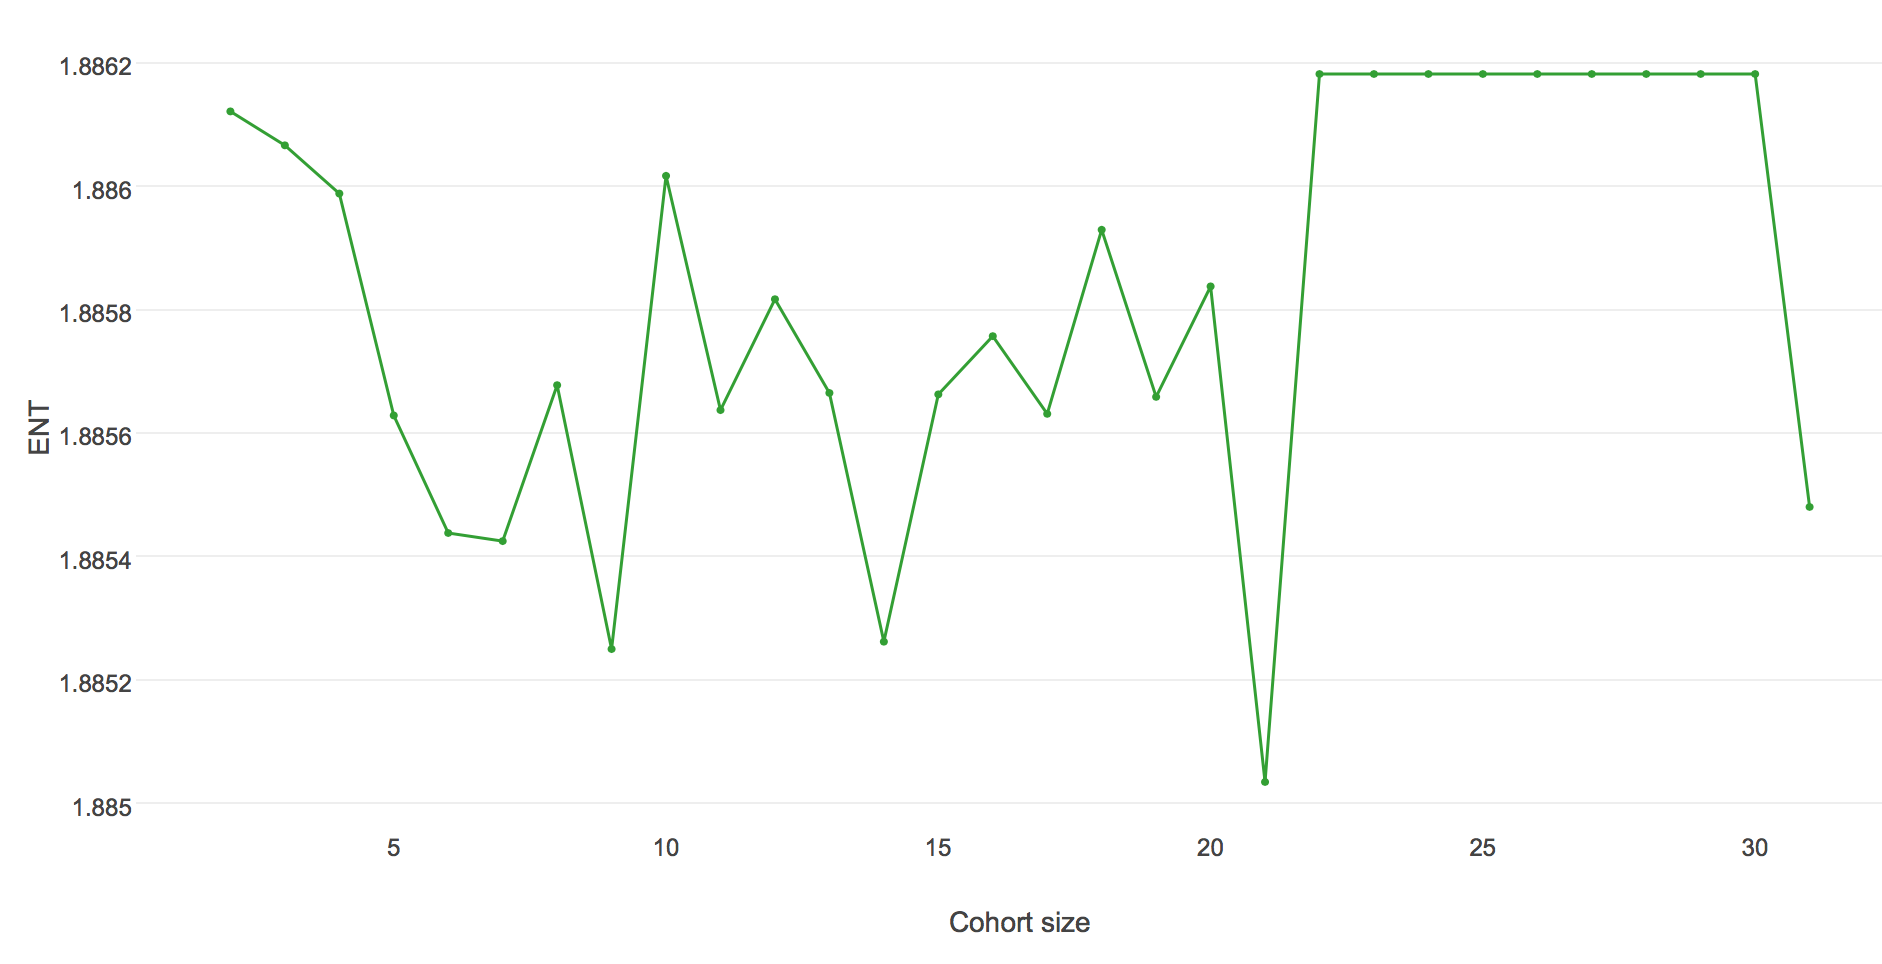
\includegraphics[width=0.8\textwidth]{dataset/grand/ent_psnm}
        \caption{Entropy of $\Pr{(score \mid nonmatch)}$ at different cohort sizes}
        \label{fig:grand_ent_psnm} %chktex 24
    \end{subfigure}%
    \caption{Grand}
    \label{fig:grand_entemd} %chktex 24
\end{figure}

\begin{figure}[htbp]
    \centering
    \begin{subfigure}[t]{\textwidth}
        \centering
        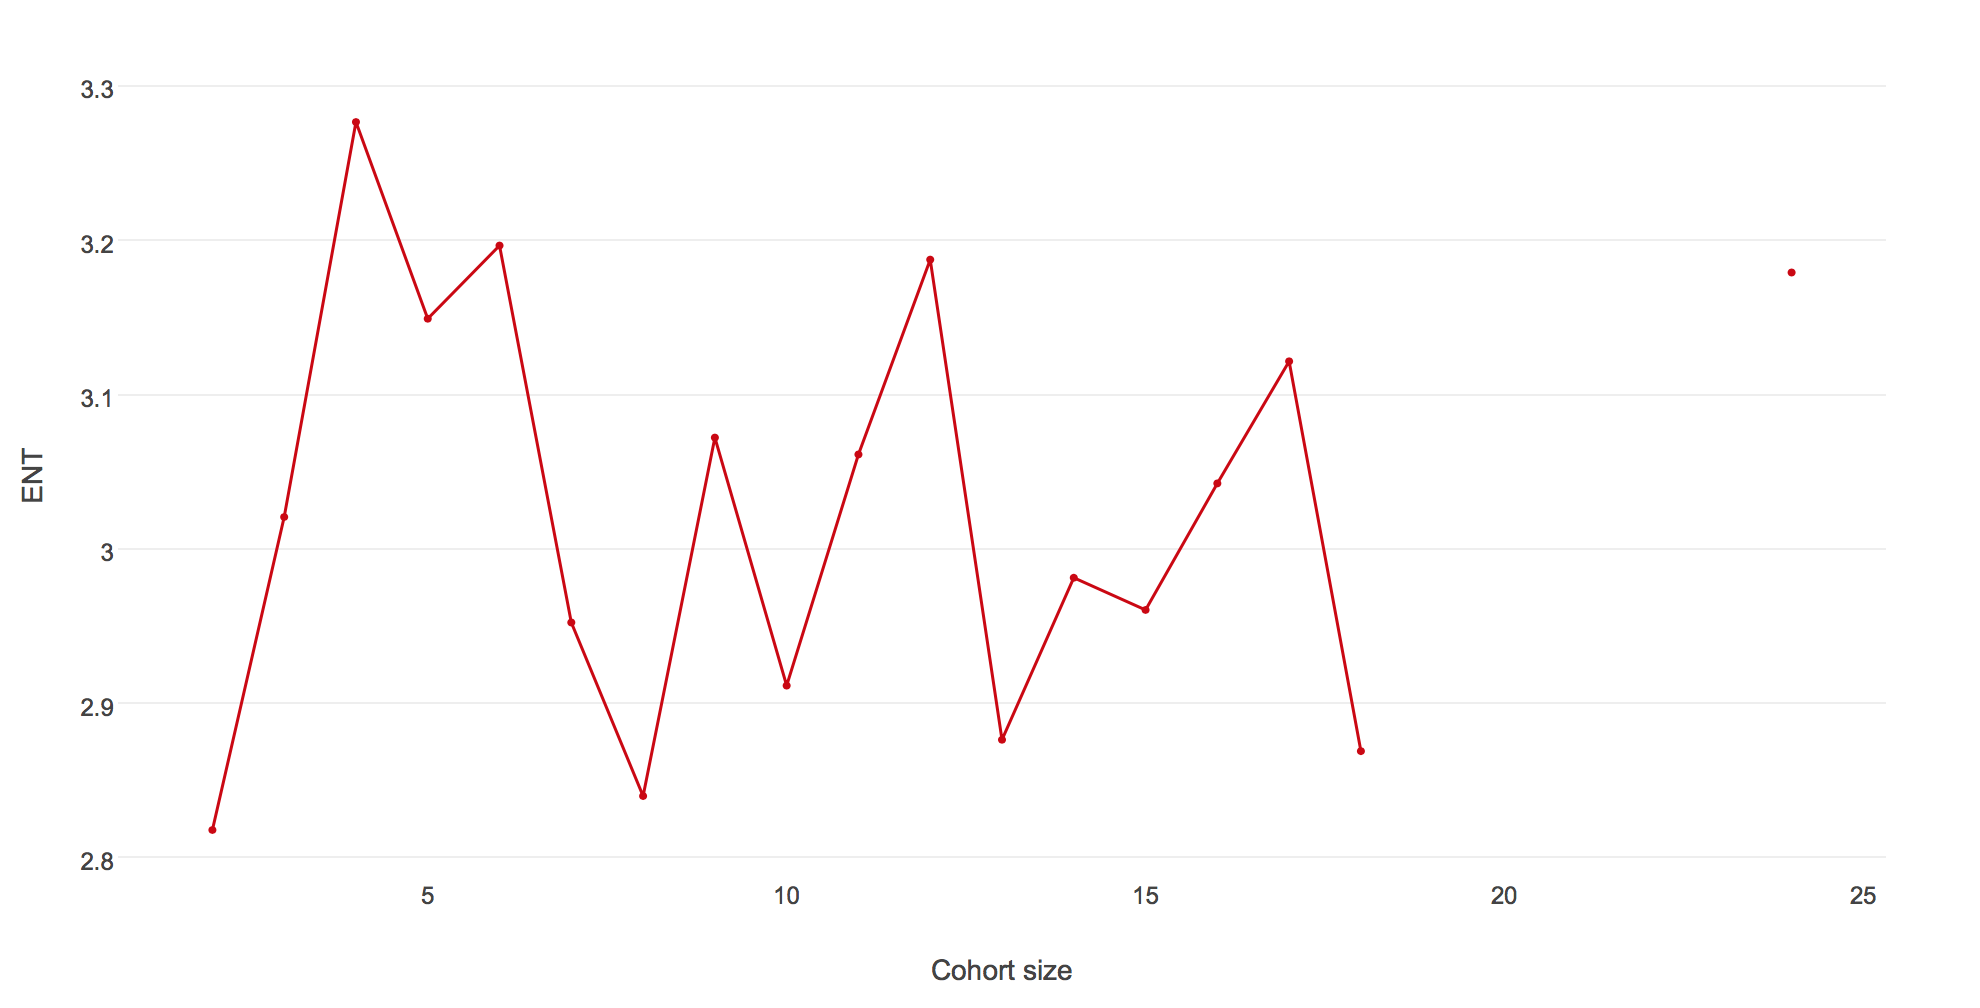
\includegraphics[width=0.8\textwidth]{dataset/otago/ent_psm}
        \caption{Entropy of $\Pr{(score \mid match)}$ at different cohort sizes}
        \label{fig:otago_ent_psm} %chktex 24
    \end{subfigure}%
    \\
    \begin{subfigure}[t]{\textwidth}
        \centering
        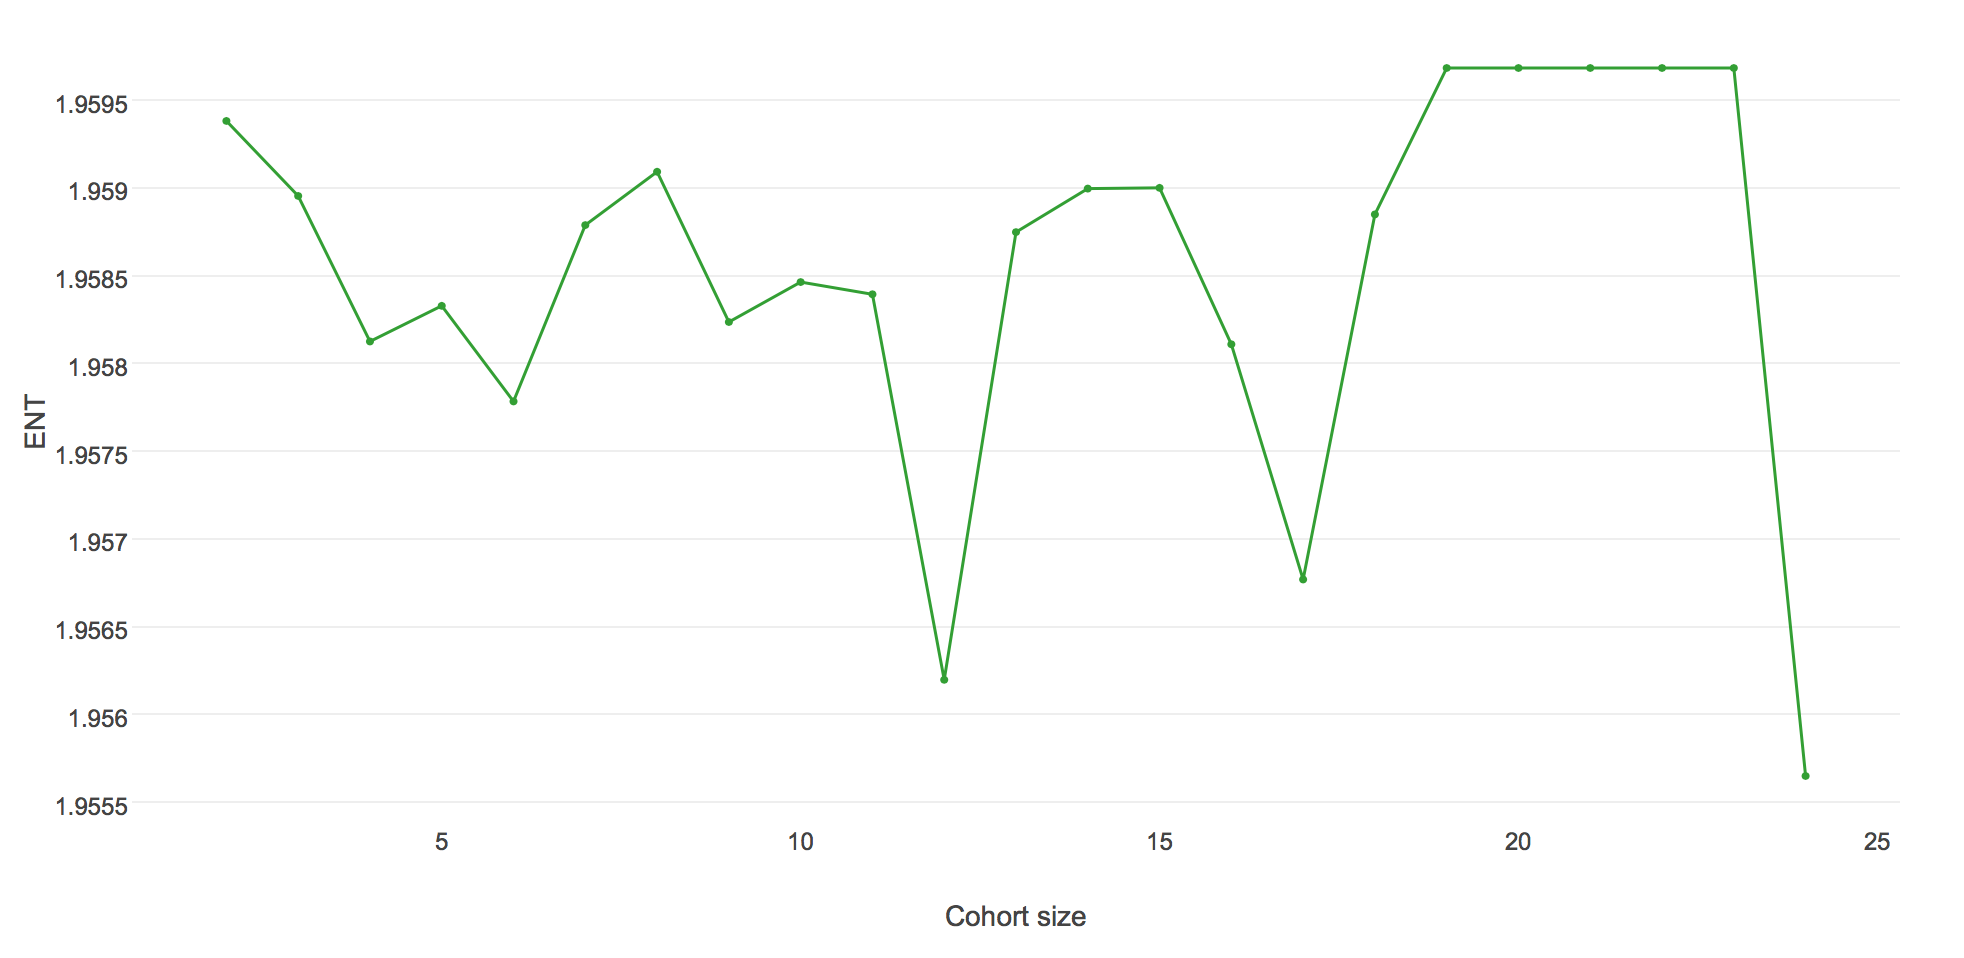
\includegraphics[width=0.8\textwidth]{dataset/otago/ent_psnm}
        \caption{Entropy of $\Pr{(score \mid nonmatch)}$ at different cohort sizes}
        \label{fig:otago_ent_psnm} %chktex 24
    \end{subfigure}%
    \caption{Otago}
    \label{fig:otago_entemd} %chktex 24
\end{figure}

\FloatBarrier%
\subsection{Probability of a Matches/Non-matches}

$$\Pr{(match \mid score)} = \frac{\Pr{(score \mid match)}\Pr{(match)}}
    {\Pr{(score)}}$$

$$\Pr{(nonmatch \mid score)} = \frac{\Pr{(score \mid nonmatch)}\Pr{(nonmatch)}}
    {\Pr{(score)}}$$

\begin{figure}[htbp]
  \begin{subfigure}[t]{\textwidth}
    \centering
    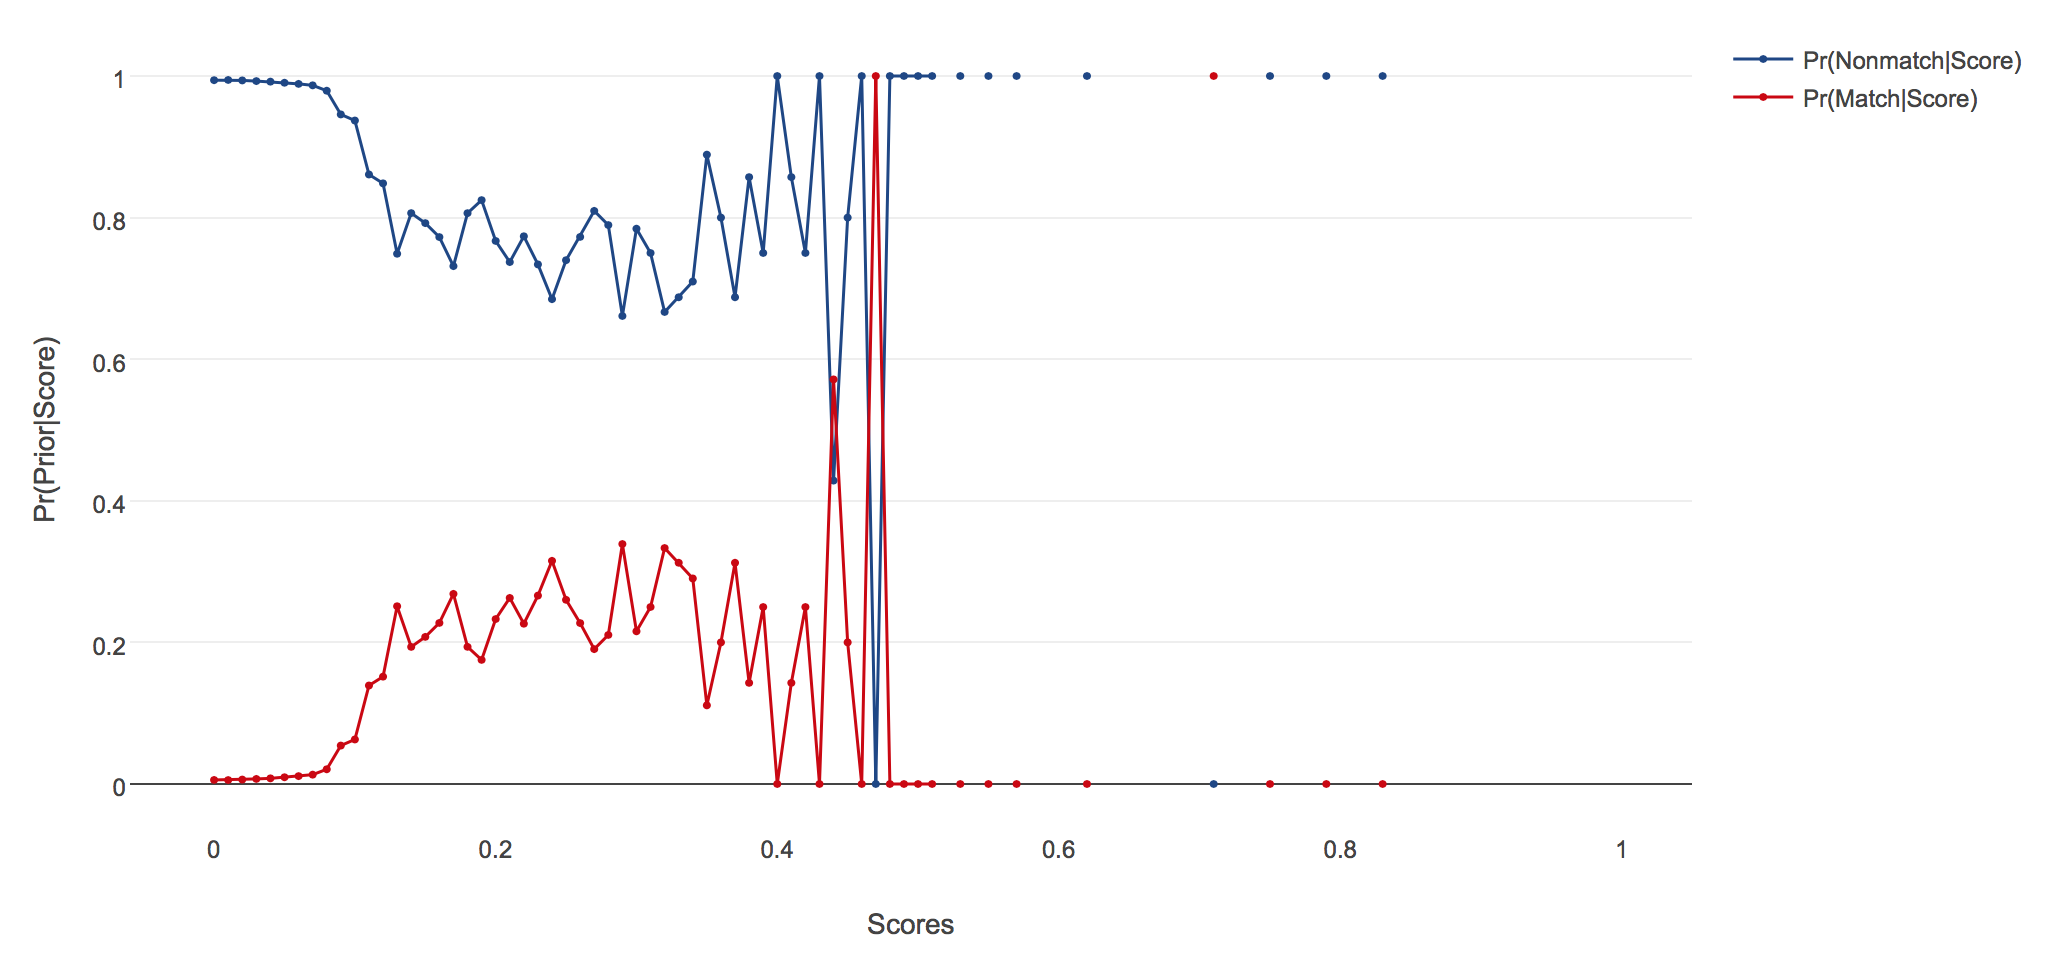
\includegraphics[width=0.8\textwidth]{dataset/grand/pms}
    \caption{Grand}
    \label{fig:grand_pms} %chktex 24
  \end{subfigure}
  \begin{subfigure}[t]{\textwidth}
    \centering
    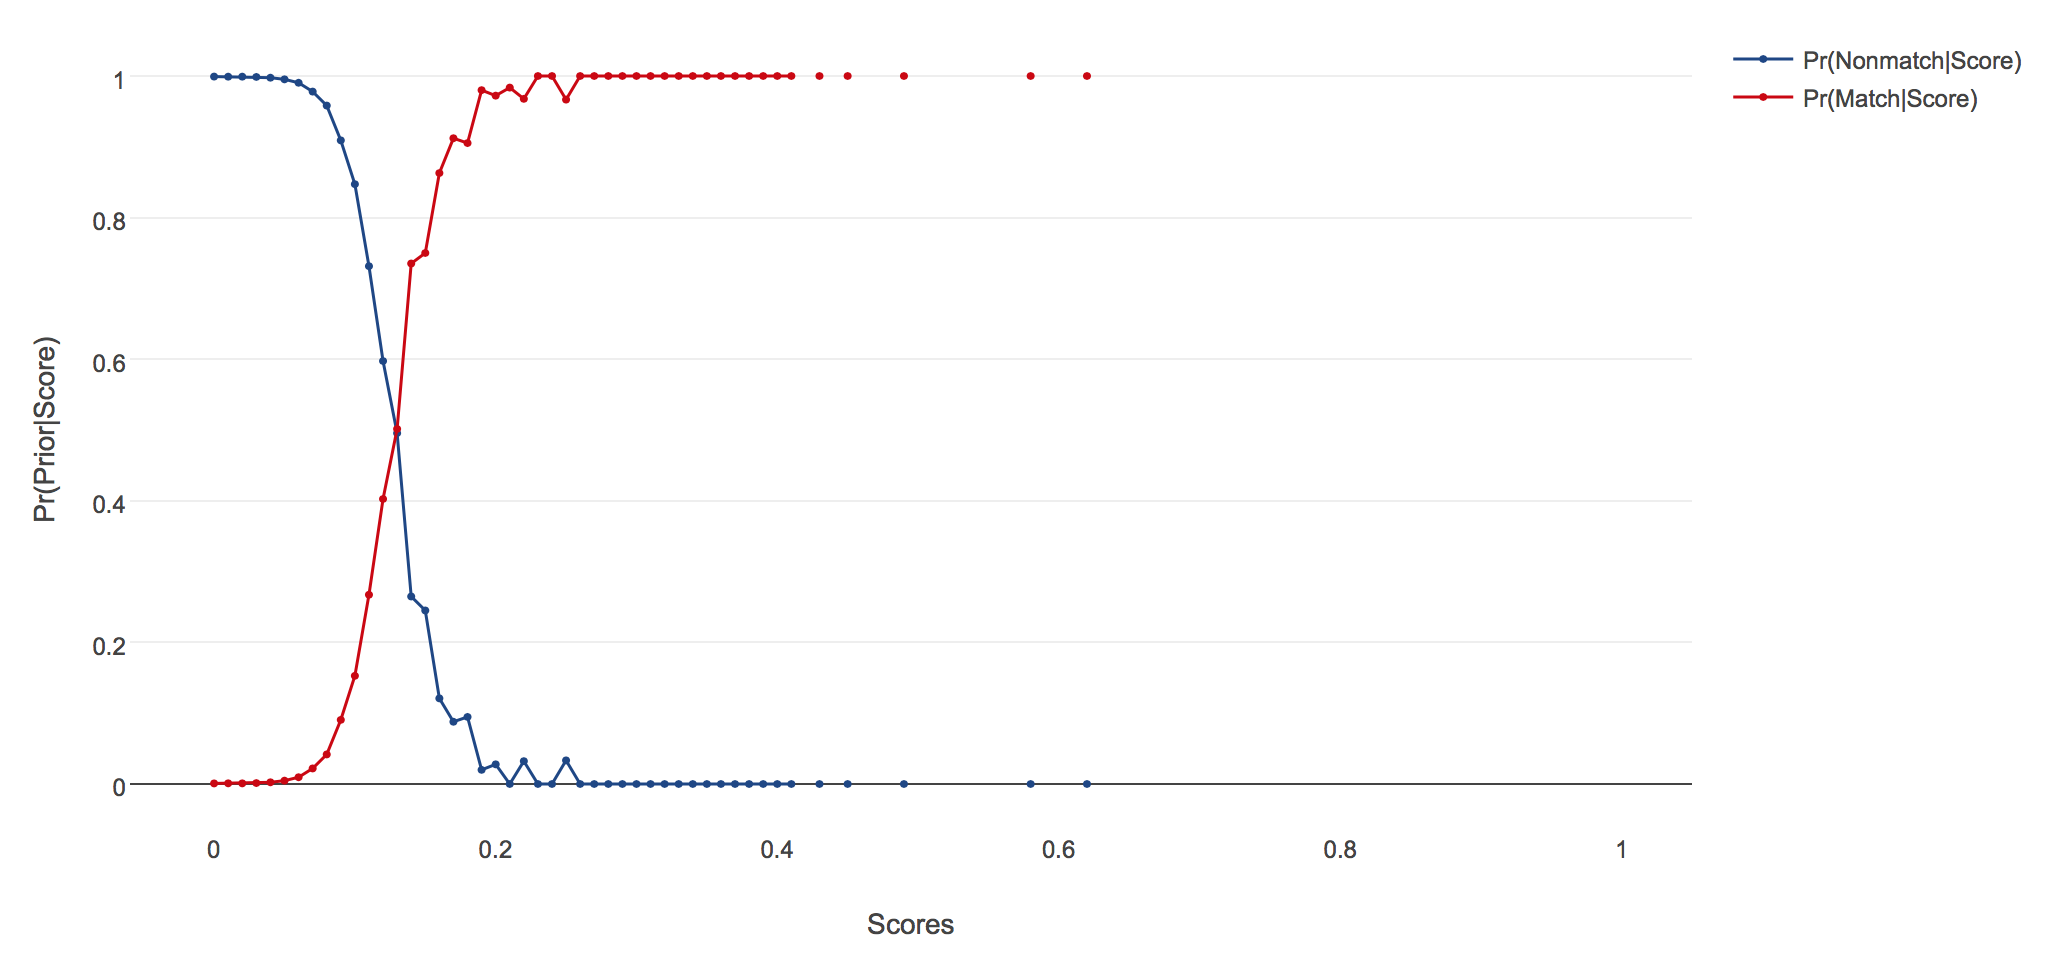
\includegraphics[width=0.8\textwidth]{dataset/otago/pms}
    \caption{Otago}
    \label{fig:otago_pms} %chktex 24
  \end{subfigure}
  \caption{Probability of matches/non-matches given score}
  \label{fig:pms}
\end{figure}

\section{Adaptive Sampling Policies} % (fold)
\label{sec:sampling_policies}

Starting with a completely unknown pairs, we would like to first get the idea
of how the overall distribution looks like. As we have seen in
Chapter~\ref{chap:relevance_feedback}, the unbiased sampling policies, such as
Uniform, and AllScores, that broadly sample the data from the distribution seem
to form a set of good candidates.

Upon the retrieval of the general distribution, we would like to adaptively
utilize the known data to determine the optimal sampling site. We experiment
with sampling from the peak of the difference between the CDF of the score
given matches and non-matches using various sampling policies.

After we get the general picture of the distribution, we repeatedly reconstruct
the plot of the difference between the CDF of the score given matches and
non-matches, then uses normal sampling policy to overlay a Gaussian
distribution, with $\mu=$\texttt{peak\_of\_the\_CDF\_difference} and
$\sigma=0.3$, on the data. We continue each cycle by the sampling probability
distribution reconstruction, and sampling from the generated distribution.
Additionally, we also use Specific sampling policy to sample specifically at the
\texttt{peak\_of\_the\_CDF\_difference} to compare the performance with the
Normal sampling policy.

\section{Results}

\begin{figure}[htb]
  \centering
  %TODO Grand
  \begin{subfigure}[t]{\textwidth}
    \centering
    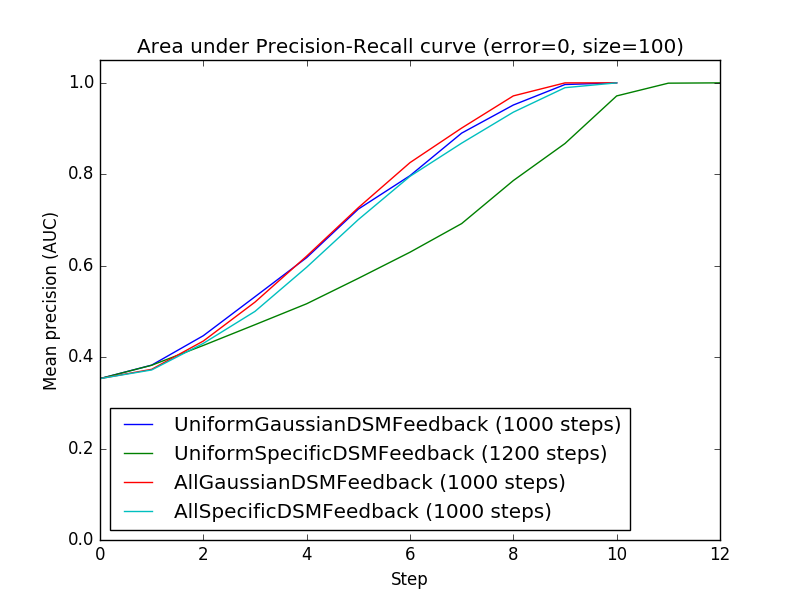
\includegraphics[width=0.6\textwidth]{otago}
    \caption{Otago}
  \end{subfigure}
  \caption{Mean Average Precision for the new sampling policies}
  \label{fig:adaptive_aoc} %chktex 24
\end{figure}

The adaptive sampling policy seem to perform averagely well. The performance
does not differ from that of the other static sampling policies we have seen in
Chapter~\ref{chap:relevance_feedback}.

% section proposed_sampling_policy (end)

% Classification with CNN
% Methodology
% * Design and Architecture
% * Population of interest and sampling subject used in the study
% * Instrument and what it measures (metrices)
% * qualifications of informants if used in the study
% * Validation
% * Data gathering procedure (experiments)
\graphicspath{{./images/chap7/}}
% Classification with CNN
% Methodology
% * Design and Architecture
% * Population of interest and sampling subject used in the study
% * Instrument and what it measures (metrics)
% * qualifications of informants if used in the study
% * Validation
% * Data gathering procedure (experiments)
\chapter{Convolutional Neural Network} % (fold)
\label{cha:convolutional_neural_network}

We first describe the our new architecture in the System Overview
(Section~\ref{sec:system_overview}). Then in the Experiments (Section~\ref{sec:experiments}), we
compare the performance of the current identification method within the
existing pattern retrieval engine with that of the new architecture.

\section{System Overview} % (fold)
\label{sec:system_overview}

In this section, we begin by presenting the architecture that outputs a
yes-or-no answer to the question whether, given two images A and B, the animal
in image A the same individual as the animal in image B.

The proposed architecture comprises two major modules shown in
Figure~\ref{fig:cnn_overview}.

\begin{figure}[htb]
  \centering
  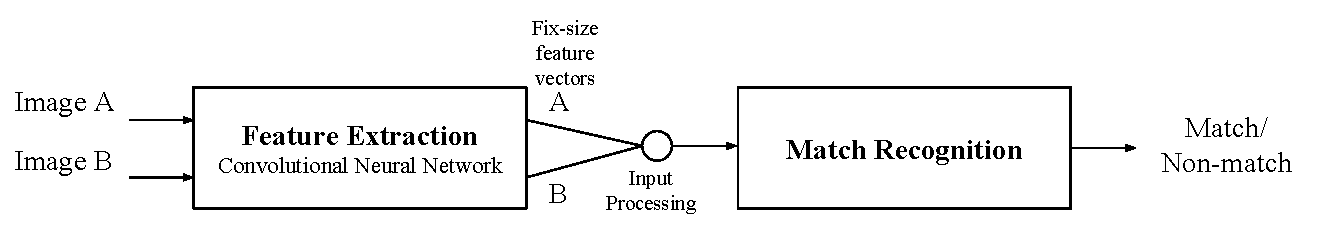
\includegraphics[width=\textwidth]{system/overview}
  \caption{System Overview}
  \label{fig:cnn_overview} %chktex 24
\end{figure}

\begin{enumerate}
  \item \textbf{Feature Extraction}. We use a pre-trained CNN with the last
  fully-connected layer, the output layer, removed to extract fix-size feature
  vectors from the input images before feeding them into the \emph{Match Recognition} module.
  \item \textbf{Match Recognition.}
\end{enumerate}

\subsection{Feature Extraction} 

For the pattern retrieving engine such as Sloop, the system continually
accumulates more data over time. The availability of abundant data enables the
learning based methods to thrive over the engineered features because they can
discover and optimize features for the specific task at hand.

Instead of hand-picking the features to learn the similarity matrices from the
data, a convolutional neural network (CNN) will be used as a feature extractor
similar to the solution proposed in~\cite{chopra05} for face verification.

We use a pre-trained CNN, AlexNet by Krizhevsky et al.~\cite{kriz12} trained on
ImageNet~\cite{imagenet}, which contains 1.2 million images with 1000
categories. To convert the CNN into a feature extractor, we strip out the last
fully-connected layer, which, in this case, outputs 1000 class scores for
ImageNet classification task. According to AlexNet architecture, this would
output a sparse 4096 dimensional vector for every images. The technique is
called transfer learning~\cite{transfer}.

We map all the available images as well as the input image to points in a low
dimensional space (4096-D compare to $227 \times 227$-D) using the
aforementioned CNN architecture. 

\begin{figure}[htbp]
  \centering
  \begin{subfigure}[t]{0.45\textwidth}
      \centering
      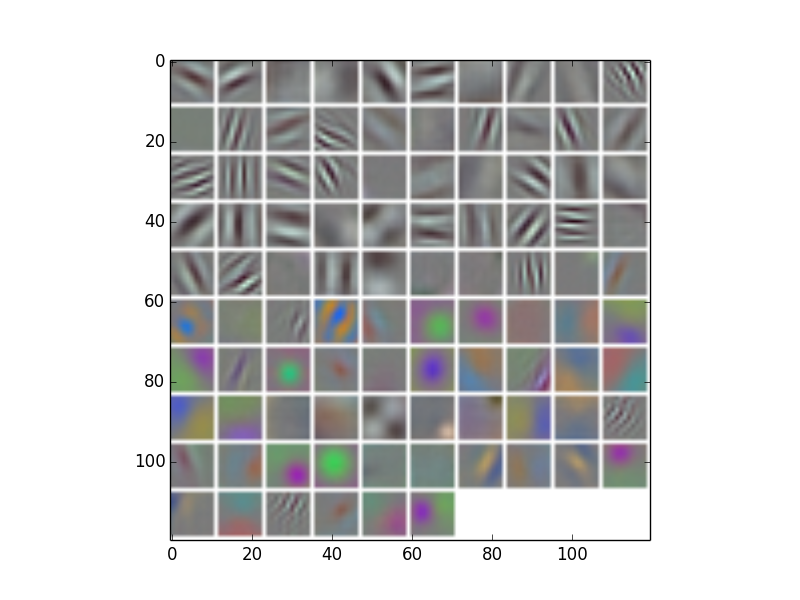
\includegraphics[width=7cm]{preprocess/paramconv1}
      \caption{The first layer filters, \texttt{conv1}}
  \end{subfigure}
  ~\\
  \begin{subfigure}[t]{0.45\textwidth}
      \centering
      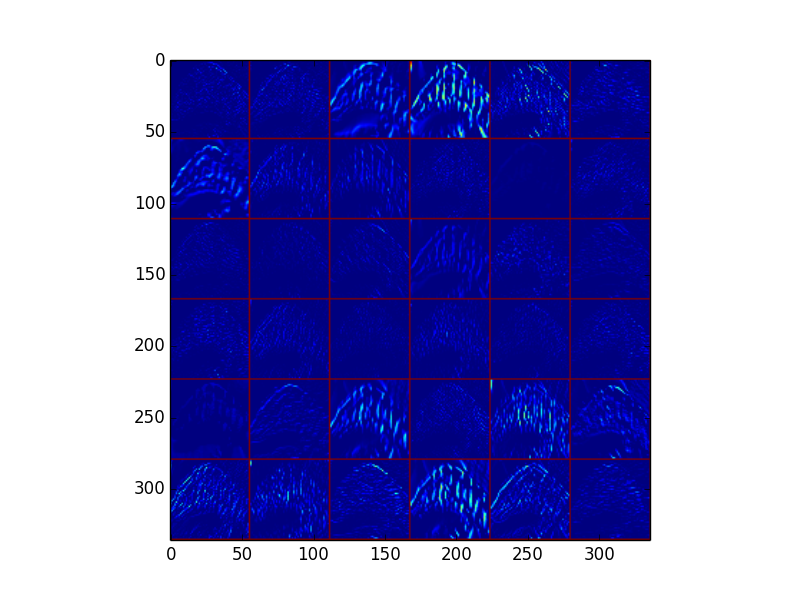
\includegraphics[width=7cm]{preprocess/blob20conv1}
      \caption{The first layer output, \texttt{conv1}}
  \end{subfigure}
  ~
  \begin{subfigure}[t]{0.45\textwidth}
      \centering
      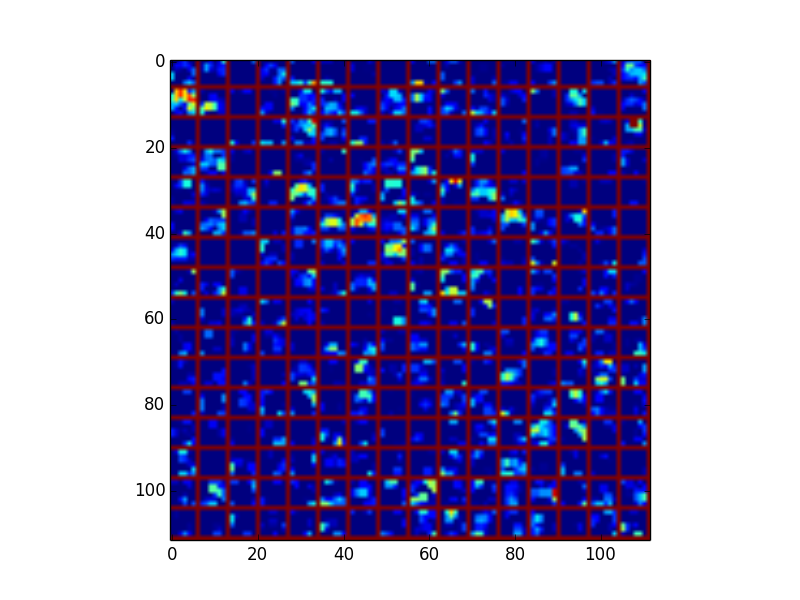
\includegraphics[width=7cm]{preprocess/blob20pool5}
      \caption{The fifth layer after pooling, \texttt{pool5}}
  \end{subfigure}
  ~ \\
  \begin{subfigure}[t]{0.45\textwidth}
      \centering
      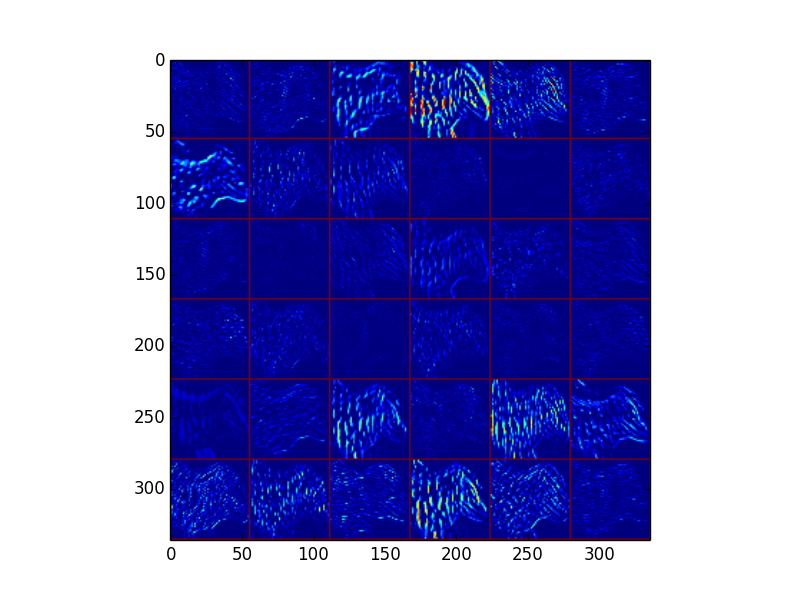
\includegraphics[width=7cm]{preprocess/lastconv1}
      \caption{The first layer output, \texttt{conv1}}
  \end{subfigure}
  ~
  \begin{subfigure}[t]{0.45\textwidth}
      \centering
      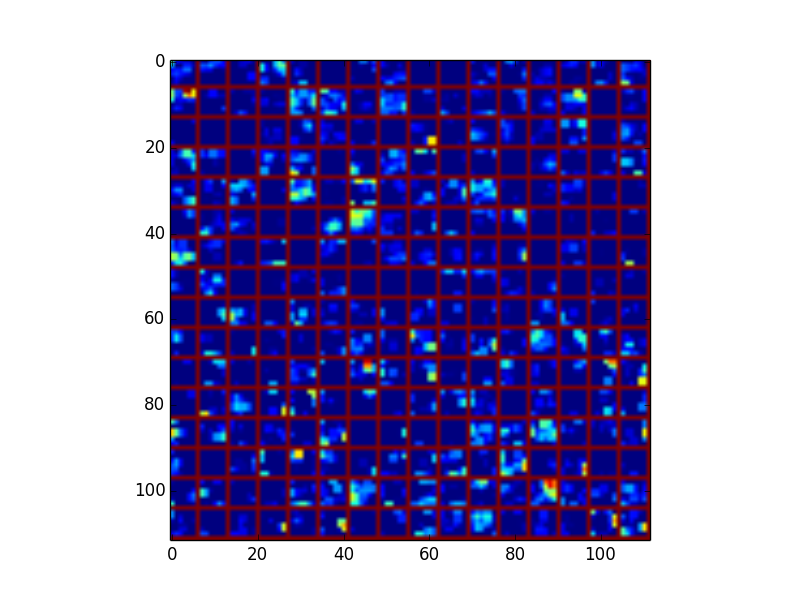
\includegraphics[width=7cm]{preprocess/lastpool5}
      \caption{The fifth layer after pooling, \texttt{pool5}}
  \end{subfigure}
  \captionsetup{justification=centering}
  \caption{Visualizing Convolutional Network layers}
\end{figure}


\textbf{Pre-trained Convolutional Neural Network}

The main advantage of using a pre-trained CNN to our application is that it is
robust to geometric distortion. This is a desirable property since the position
of the individuals in our dataset are not aligned. This enables us to
accurately recognize the animal regardless of its position in the image. 

The translation invariant property emerges as a result of the contiguity in our
pooling regions and the fact that we only pool features generated from the same
hidden units~\cite{ufldl}. Even though the property is desirable to reduce the
translation noise, this disallows learning some features that are described by
their relative positions. For example, individual A with a star-shaped spot
right above its eye may be confused with another individual B who also has
star-shaped spot underneath its eye. 

The solution to such problem is to experiment with different pattern of pooling
regions, and relax the parameter sharing scheme. Since we are using an existing
pre-trained architecture, it is hard to tailor to fit our data. The improvement
can be included in the future work~\ref{cha:future_work}.

\textbf{Caffe}

The CNN is implemented in python using Caffe~\cite{caffe}, a deep learning
framework developed by the Berkeley Vision and Learning Center (BVLC).

\subsection{Match Recognition}

Once we have the 4096-D vectors for all images generated from our CNN feature
extractor, we transfer them into a second target match recognizer and train it
on a target dataset and task. The match recognizer is a linear classifier that,
given a pair of image vectors, decides whether the two images contains the same
individual.

\textbf{Input Processing}

Upon receiving the input from the feature extractor, we process the input using
one of the two method before passing it into the recognizer which outputs a
binary label determining whether (A, B) is a match.

\begin{enumerate}
\item Concatenation

Given two input image vectors $\vec{A}$ and $\vec{B}$ (flattened), we
concatenate them horizontally so that the output $\vec{E}$ becomes $$\vec{E} =
[ \vec{A}\, \vec{B} ].$$ To make the order deterministic, we always start with
the vector with smaller sum; otherwise, if equal sum, we compare each pair of
corresponding entries in both vectors until we find an entry with a smaller
element.

We can visualize this as feeding a tuple of image vectors $( \vec{A}, \vec{B}
)$ to a linear classifier. This is equivalent to giving the classifier all the
information we have and expect it to figure out the optimal parameters.
However, in this case there is no separator indicating that two image vectors
are actually separated.

\item Computing the absolute difference

We would like to find a similarity metric that represents how much two images
differ from each other. In order to achieve that we come up with following
metric:
$$\vec{E} = |\vec{A} - \vec{B}|$$
Each entries $e_i \in \vec{E}$ is
small if $\vec{A}$ and $\vec{B}$ belong to the same category, and large if
different.  Not only this encapsulates the desired numerical behavior, but it
also eliminates the absence of separator problem.
  
\end{enumerate}

\textbf{Recognizer}

Images can be uploaded to Sloop one by one or in a batch. One major difference
is that the batch processing keeps the system weights constant while computing
the error associated with each sample in the input, whereas the on-line version
constantly updates its weights. For the real-time system like Sloop, we would
prefer the on-line version of the classification algorithm given the same
classification performance.

We have implemented following algorithms as our match recognizer:
\begin{itemize}
  \item Linear support vector machine (SVM) with L2 regularization (squared
    Euclidean norm)
  \item SVM with radial basis function kernel (SVM-RBF), L2 regularization
  \item Perceptron (P)
  \item Passive-Aggressive with hinge loss (PA-I)
  \item Passive-Aggressive with squared hinge loss (PA-II)
\end{itemize}

We compare the performance of each classifier in the Experiments
section~(\ref{sec:experiments}). The classifier with the best performance will be
selected for our final design.
% section system_overview (end)

\section{Experiments} % (fold)
\label{sec:experiments}

In this section, we first introduce the datasets used in the experiments, then
present the detailed evaluation of the variants of our architecture and the
comparison between the presented solutions.

\subsection{Dataset}

The training and testing data is available in the existing Sloop system. We
base our experiments on both species of skinks: \emph{Grand} and \emph{Otago}
mentioned in Chapter~\ref{cha:datasets}.

For our experiments, each image from both databases is reduced to the size of
$227 \times 227$ pixels so that it can be directly fed into the CNN
architecture to speed up the feature extraction. Regardless of our preprocess,
the CNN will resize the images into $227 \times 227$ to fit its input
dimension. However, resizing is not necessary because practically our system
should maintain its identification capability without regard to the variations
in sizes, lighting, or background.

\textbf{Partitioning}

We divide the data from both databases into four datasets by animal species:
Gr$^{L}$-I, Gr$^{L}$-II, Ot$^{L}$-I, Ot$^{L}$-II where Gr is Grand, Ot is
Otago, $L$ is left view. Notice that the right view is not be used for the
experiments because the results should be similar to that of left view by
symmetry. In addition, due to our memory limit during the processing, each
dataset contains only 300 images of individuals whose image per individuals are
greater than 11.

For the purpose of generating a test set that resembles the empirical input and
another test set with images that are not seen before during training, we build
our datasets using two different techniques.
\begin{itemize}
  \item Gr$^{L}$-I, Ot$^{L}$-I represents the empirical input where the data in
  the test set can also be seen in the training set.
  \item Gr$^{L}$-II, Ot$^{L}$-II represents the test set with images that are
  not seen before during training. The set of individuals is split into three
  disjoint sets for training, validating, and testing. Each images in a set can
  only be paired with the images within the same set.
\end{itemize}

For each dataset, we partition the set of the \emph{generated pairs} into three
sets: train set (60\%), validation set (20\%), and test set (20\%) respectively.
We prevent overfitting problem by monitoring the model's performance on a
validation set, acting as a representative of future test examples. If the
model's performance ceases to improve sufficiently on the validation set then
we test the model on teh actual test set.


\begin{table}[t]
\captionsetup{justification=centering}
  \caption{Details of the train, validation, and test set for the four datasets}
\centering
  \begin{tabular}{llrcc}
    \toprule
    \multicolumn{2}{l}{Name (NTotal)}      & NPairs & \% Match & \% Non-match \\
    \midrule
    \multirow{3}{*}{Gr$^{L}$-I (10878)}  & Train & 6526 & 0.07 & 0.93 \\
                                 & Val   & 2175 & 0.07 & 0.93 \\
                          & Test  & 2177 & 0.07 & 0.93 \\
\midrule
\multirow{3}{*}{Ot$^{L}$-I (10878)}  & Train & 6526 & 0.06 & 0.94 \\
                                 & Val   & 2175 & 0.06 & 0.94 \\
                                 & Test  & 2177 & 0.06 & 0.94 \\
\midrule
  \multirow{3}{*}{Gr$^{L}$-II} & Train & 2926 & 0.13 & 0.87\\
                                 & Val   & 351 & 0.38 & 0.62\\
                                 & Test  & 1035 & 0.25 & 0.75\\
    \midrule
    \multirow{3}{*}{Ot$^{L}$-II} & Train & 3240 & 0.10 & 0.90\\
                                 & Val   & 561 & 0.31 & 0.69\\
                                 & Test  & 561& 0.26 & 0.73\\
    \bottomrule
  \end{tabular}
  \label{tab:results_tvt}
\end{table}
% section experiments (end)

% chapter convolutional_neural_network (end)
% Analysis and Interpretation of data
% * meaning
% * in the studies involving
% * interconnection among data
% * Check for indicaotr whether hypothesis is supported by he finding
% * Link present finding to previous liturature
% Analysis and Interpretation of data
% * meaning
% * in the studies involving
% * interconnection among data
% * Check for indicator whether hypothesis is supported by he finding
% * Link present finding to previous literature
\chapter{Analysis and Interpretation}

\section{Convolutional Neural Network}

\subsection{Recognition}

To evaluate the initial results, we calculate precision, recall, and F1 values
of the predicted results compare to the gold standard annotated by the
biologists.

\textbf{Input Processing}

According to the proposed architecture in Section~\ref{sec:system_overview}, we have
experimented with both method of input processing, namely, concatenation and
computing the difference. The results are shown in
Table~\ref{tab:concatenation_table} and Table~\ref{tab:results_table}.


\begin{table}[t]
\captionsetup{justification=centering}
  \caption{Precision (P), recall (R), and F-score (F) of the classification
  results for the input processing with feature vectors concatenation}
  \label{tab:concatenation_table} %chktex 24
\centering
% The 'C' column type is defined in the document preamble. It adds
% extra space to the left of the column to replace vertical rules. The
% 'H' column type is for headers above it, which need to account for
% the extra space.
\begin{tabular}{llCccCccCcc}
    \toprule
    \multicolumn{2}{c}{\multirow{2}{*}{Dataset} } & \multicolumn{3}{H}{PCT} &
        \multicolumn{3}{H}{PA-I} & \multicolumn{3}{c}{PA-II}\\
  \cmidrule{3-11}
        & & P & R & F  & P & R & F  & P & R & F \\
    \midrule
    \multirow{3}{*}{Gr$^{L}$-I}  & Train & 0.01 & 0.03 & 0.01 & 0.04 & 0.01 
        & 0.01 & 0.00 & 0.00 & 0.00 \\
                                 & Val   & 0.40 & 0.13 & 0.08 & 0.23 & 0.06
        & 0.08 & 0.46 & 0.08 & 0.06 \\
                                 & Test  & 0.01 & 0.05 & 0.02 & 0.03 & 0.01
        & 0.01 &  0.00 & 0.02 & 0.01 \\
    \bottomrule
  \end{tabular}
\end{table}

All the classifiers perform poorly when feature vectors concatenation is used
as the input processing method. This happens because of the \emph{curse of
dimensionality}, where there are too many unnecessary input features. Doubling
the dimension of the input image vector overcomplicates the classifier
parameters causing the downfall in the prediction accuracy. On the other hand,
the classifiers tend to perform pretty well when using absolute feature
difference as the input.

\afterpage{%
    \clearpage% Flush earlier floats (otherwise order might not be correct)
    \thispagestyle{empty}% empty page style (?)
    \begin{landscape}% Landscape page
    \begin{table}
      \captionsetup{justification=centering}
        \caption{Precision (P), recall (R), and F-score (F) of the linear
        classifier with absolute feature difference on train, validation, and
        test set of the four datasets}
        \label{tab:results_table} %chktex 24

      \centering % Center table
        % The 'C' column type is defined in the document preamble. It adds
        % extra space to the left of the column to replace vertical rules. The
        % 'H' column type is for headers above it, which need to account for
        % the extra space.
      \hskip-2.0cm\begin{tabular}{llCccCccCccCccCcc}
          \toprule

          \multicolumn{2}{c}{\multirow{2}{*}{Dataset} } & \multicolumn{3}{H}{SVM}
            & \multicolumn{3}{H}{SVM-RBF} & \multicolumn{3}{H}{PCT}
            & \multicolumn{3}{H}{PA-I} & \multicolumn{3}{c}{PA-II}\\
        \cmidrule{3-17}
                                                    & & P & R & F  & P & R & F 
                                                    & P & R & F  & P & R & F & P
                                                    & R & F \\
          \midrule
          \multirow{3}{*}{Gr$^{L}$-I}  & Train & 0.91 & 0.21 & 0.34 & 0.97 & 0.18
            & 0.30 & 0.40 & 0.26 & 0.32 & 0.57 & 0.31 & 0.29 & 0.57 & 0.29 & 0.30
            \\
                                       & Val   & 0.95 & 0.23 & 0.37 & 0.99 & 0.19
                                       & 0.32 & 0.58 & 0.37 & 0.45 & 0.65 & 0.48
                                       & 0.38  & 0.67 & 0.44 & 0.39      \\
                                       & Test  & 0.82 & 0.20 & 0.33 & 1.00 & 0.21
                                       & 0.35 &  0.42 & 0.24 & 0.30 & 0.54
                                       & 0.33 & 0.28 & 0.52 & 0.29 & 0.28     \\
          \midrule
          \multirow{3}{*}{Ot$^{L}$-I}  & Train & 0.64 & 0.24 & 0.32 & 0.88 & 0.21
          & 0.34  & 0.45 & 0.32 & 0.29 & 0.37 & 0.16 & 0.23 & 0.36 & 0.27
          & 0.30     \\
                                       & Val   & 0.81 & 0.42 & 0.51 & 0.90 & 0.24
                                       & 0.37 & 0.55 & 0.54 & 0.42 & 0.89 & 0.30
                                       & 0.39 & 0.65 & 0.55 & 0.59     \\
                                       & Test  & 0.66 & 0.26 & 0.33 & 0.90 & 0.20
                                       & 0.32 & 0.46 & 0.39 & 0.33 & 0.36 & 0.17
                                       & 0.23 & 0.42 & 0.32 & 0.36     \\
          \midrule
          \multirow{3}{*}{Gr$^{L}$-II} & Train & 0.92 & 0.35 & 0.50 & 0.99 & 0.21
          & 0.34 & 0.99 & 0.27 & 0.43 & 0.89 & 0.48 & 0.63 & 0.83 & 0.57 & 0.67 
          \\
                                       & Val   & 0.79 & 0.20 & 0.32 & 1.00 & 0.20
                                       & 0.33 & 0.93 & 0.19 & 0.32 & 0.76 & 0.21
                                       & 0.33 & 0.66 & 0.24 & 0.36     \\
                                       & Test  & 0.85 & 0.22 & 0.35 & 1.00 & 0.18
                                       & 0.30 & 0.92 & 0.19 & 0.31 & 0.86 & 0.20
                                       & 0.32 & 0.69 & 0.22 & 0.34     \\
          \midrule
          \multirow{3}{*}{Ot$^{L}$-II} & Train & 0.57 & 0.29 & 0.38 & 1.00 & 0.22
          & 0.38 & 0.53 & 0.70 & 0.60 & 0.59 & 0.78 & 0.67 & 1.00 & 0.25
          & 0.40     \\
                                       & Val  & 0.57 & 0.68 & 0.62 & 1.00 & 0.24
                                       & 0.39 & 0.53 & 0.37 & 0.43 & 0.56 & 0.30
                                       & 0.39 & 0.97 & 0.19 & 0.32   \\
                                       & Test  & 0.57 & 0.28 & 0.38  & 1.00
                                       & 0.19 & 0.32 & 0.43 & 0.36 & 0.39 & 0.50
                                       & 0.32 & 0.39 & 1.00 & 0.22 & 0.37     \\
          \bottomrule
        \end{tabular}
      \end{table}
    \end{landscape}
    \clearpage% Flush page
}

Considering the classification results in Table~\ref{tab:results_table}, all the
classifiers seem to perform equally well on the test data considering the
F-beta score. SVM with radial bas kernel function yields the most stable
performance with very high precision for both species. The offline algorithms
slightly outrun all the online ones on average.

In the system such as Sloop, we would like to have a high standard on the
individuals marked as a match because mistakes are extremely detrimental. It
can easily propagate over the whole database so we would like to select a
classifier with high F-beta score, preferably with high precision. In general,
SVM-RBF is a very safe choice. However, the classifier with highest F-beta
score are listed as following:

\begin{itemize}
  \item Gr$^{L}$-I SVM-RBF
  \item Ot$^{L}$-I PA-II/SVM/SVM-RBF (Even though PA-II yields highest F-score,
  its precision is very low.)
  \item Gr$^{L}$-II SVM
  \item Ot$^{L}$-II PCT/PA-I/SVM
\end{itemize}

Species-wise, classification results for Otago skinks seem to have higher
recall, but lower precision, than that of Grands despite the similar proportion
between the matching and non-matching pairs in training, validation, and test
sets. This implies that the feature vectors of Otago are pretty similar to one
another in the classifiers' point of view. The similarity results from the
visual patterns of the species, which are less detailed compared to Grand.

% Conclusion
% * Describe each problem, research design, and findings (ans to prob)
% * Recommendations
% Conclusion
% * Describe each problem, research design, and findings (ans to prob)
% * Recommendations
\chapter{Conclusion}

We have implemented additional two extensions to Sloop to improve the
classification performance.

\section{Relevance Feedback} A relevant feedback simulator and the crowdsourced
relevance feedback integration of Sloop, Sloop MTurk, have been implemented to
study the impact of relevance feedback on the ranked retrieval data as well as
improve the correctness of the result sets. The experiments have confirmed that
relevance feedback dramatically accretes precision and recall, despite the
present of errors. We showed certain sampling methods outperform others in term
of the cost. Exploiting the accumulation of the retrieved information, we
introduced a new sampling method that takes advantage of the difference between
the CDF of score given matches/non-matches. We then compare the performance of
our adaptive sampling approach to the other static  approaches.

\section{Convolutional Neural Network}

We presented a new architecture for learning similarity metric in a large
dataset and experimented with several algorithm to find the solution that best
suited for our animal identification scheme. 

We propose a new architecture that comprises a feature extractor and a match
recognizer. The feature extractor is implemented by a pre-trained convolutional
network, AlexNet, with the output layer removed. Given a pair of two images,
the feature extractor outputs two fix-size feature vectors. We then take the
absolute difference of the feature vector and pass the resulting vector into a
support vector machine classifier, which has been proved to be most robust and
suitable model in our application. Finally, the classifier outputs whether the
two images contains the same individual animals. According to the results, it
is able to achieve very high precision with good recall while being completely
automated and independent from human involvement. 


% Conclusion
% * Describe each problem, research design, and findings (ans to prob)
% * Recommendations
\chapter{Future Work}

\section{Convolutional Neural Network}

One possible improvement is to tailor and train the parameters of the Convolutional Network to best fit our data. However, this requires a much larger dataset of labeled images. Therefore, we need to increase the size of our dataset.

In order to properly evaluate the new system performance, we should use the SIFT algorithm in the previous system as our baseline. We have already generated the SIFT object representing each images available in the system however, they are generated from a sets of keypoints that are manually marked so that it is able to acheives 99.99\% ranking accuracy. With such biase, it is hard to evaluate the relative performance between the new and the old system.

Further, we can evaluate the performance of the model by analyzing the receiver operating characteristics (ROC), or ROC curves, which illustrates the performance of a classifier model. ROC exhibits the relationship between true positive rate (TPR) and the false positive rate (FPR), which provides tools to select possibly optimal models and to discard suboptimal ones.

Since the datasets contain the human input, the manual input data can be utilized to improve the identification result as a one of the features. The definition of number of human interaction depends on the action required to complete a specific classification task. For instance, if the classification task requires user to click on the photos, the number of user clicks will then determine the number of human interaction. The classification results of the completely automated feature extractor and semi-automated feature extractor should be compared to determine the optimal human involvement.


\appendix
Suppose each HIT is distributed to $n$ workers, or in other words, each HIT
contains $n$ assignments and there are $m$ questions for each assignments.  For
each assignment, the chance that an assignment is accepted with an incorrect
answer to the unknown pair is $\frac{1}{2^m}$, and the chance that an assignment
is rejected is $\epsilon_m = (1-\frac{1}{2^{m-1}})$

The probability that only one assignment out of $n$ assignments is accepted with
an incorrect answer to the unknown pair is
$$\epsilon_m^{n-1} \cdot \frac{1}{2^m}$$
The probability that two assignments are accepted, but the resulting answer to
the unknown pair is incorrect is
$$\epsilon_m^{n-2} \cdot \binom{2}{2}\frac{1}{2^{2\cdot m}}$$
if both are incorrect, and
$$\epsilon_m^{n-2} \cdot \binom{2}{1}\frac{1}{2^{2\cdot m}}$$
if both answers are `do not match' and the actual answer is the same.
The error rate in this case is thus
$$3 \cdot \epsilon_m^{n-2} \cdot \frac{1}{2^{2\cdot m}}$$
if both answers are `do not match' and the actual answer is the same.
The probability that three assignments are accepted, but the resulting answer to
the unknown pair is incorrect is
$$\epsilon_m^{n-3} \cdot \binom{3}{3}\frac{1}{2^{3\cdot m}}$$
if all are incorrect, and
$$\epsilon_m^{n-3} \cdot \binom{3}{2}\frac{1}{2^{3\cdot m}}$$
if two are incorrect.
The error rate in this case is thus
$$4 \epsilon_m^{n-3} \cdot \frac{1}{2^{3\cdot m}}$$
if two are incorrect.
Let $i$ be the number of assignments accepted and
$\epsilon_{nm} = \frac{1}{2^m\epsilon_m}$.
The error rate can be generalized as follows:
\begin{description}
  \item[$i$ is odd:]
  $$(\binom{i}{i} + \binom{i}{i-1} + \cdots +
  \binom{i}{\frac{i+1}{2}})\epsilon_{nm}^i \epsilon_m^n$$
  \item[$n$ is even:]
  $$(\binom{i}{i} + \binom{i}{i-1} + \cdots +
  \binom{i}{\frac{i}{2}})\epsilon_{nm}^i \epsilon_m^n$$
\end{description}
By the binomial theorem, the total error rate is bounded by

When the only person whose assignment is correct
% \chapter{Figures}

% \vspace*{-3in}

% \begin{figure}
% \vspace{2.4in}
% \caption{Armadillo slaying lawyer.}
% \label{arm:fig1}
% \end{figure}
% \clearpage
% \newpage

% \begin{figure}
% \vspace{2.4in}
% \caption{Armadillo eradicating national debt.}
% \label{arm:fig2}
% \end{figure}
% \clearpage
% \newpage

%% This defines the bibliography file (main.bib) and the bibliography style.
%% If you want to create a bibliography file by hand, change the contents of
%% this file to a `thebibliography' environment.  For more information 
%% see section 4.3 of the LaTeX manual.
\begin{singlespace}
\bibliography{main}
\bibliographystyle{plain}
\end{singlespace}

\end{document}

